
\documentclass{article}

% === Básico ===
\usepackage[utf8]{inputenc} % opcional en LaTeX moderno
\usepackage[english]{babel}

\usepackage[left=2.5cm,right=2.5cm,top=3cm,bottom=3cm]{geometry}
% OJO: no usar vmargin junto con geometry
% \usepackage{vmargin}  % <-- QUITAR
% \setmargins{...}      % <-- QUITAR

\usepackage{graphicx}
\usepackage{amsmath,amssymb,amsfonts}
\usepackage{array,multirow,float}
\usepackage{enumitem}
\usepackage{chngcntr}
\usepackage{blindtext}
\usepackage{verbatim}
\usepackage{ifoddpage}
% \usepackage{breqn}    % <- Suele dar problemas con amsmath; si no lo usás, mejor quitarlo.

% === TikZ / PGFPlots (arregla 'name path' & fillbetween) ===
\usepackage{tikz}
\usetikzlibrary{calc,intersections,shapes.geometric,datavisualization.formats.functions}
\usepackage{pgfplots}
\usepgfplotslibrary{polar,fillbetween}
\pgfplotsset{compat=1.18} % usa 1.17 si tu TeX es más viejo

% === Colores & enlaces ===
\usepackage{xcolor} % mejor que 'color'
\usepackage{hyperref}
\hypersetup{
  colorlinks=true,
  linkcolor=teal,
  urlcolor=teal,
  citecolor=teal
}

% === Bibliografía (biber) ===
\usepackage{csquotes}
\usepackage[style=authoryear,sorting=nyt,backend=biber]{biblatex}
% Usa ruta relativa o barras normales si es absoluta:
% \addbibresource{E:/articulos/LATEX/test/bibliography.bib}
\addbibresource{bibliography.bib}

% --- (tus overrides para enlazar título/año; los dejo tal cual) ---
\DeclareCiteCommand{\cite}
  {\usebibmacro{prenote}}
  {\usebibmacro{citeindex}\printtext[bibhyperref]{\usebibmacro{cite}}}
  {\multicitedelim}
  {\usebibmacro{postnote}}

\DeclareCiteCommand*{\cite}
  {\usebibmacro{prenote}}
  {\usebibmacro{citeindex}\printtext[bibhyperref]{\usebibmacro{citeyear}}}
  {\multicitedelim}
  {\usebibmacro{postnote}}

\DeclareCiteCommand{\parencite}[\mkbibparens]
  {\usebibmacro{prenote}}
  {\usebibmacro{citeindex}\printtext[bibhyperref]{\usebibmacro{cite}}}
  {\multicitedelim}
  {\usebibmacro{postnote}}

\DeclareCiteCommand*{\parencite}[\mkbibparens]
  {\usebibmacro{prenote}}
  {\usebibmacro{citeindex}\printtext[bibhyperref]{\usebibmacro{citeyear}}}
  {\multicitedelim}
  {\usebibmacro{postnote}}

\DeclareCiteCommand{\footcite}[\mkbibfootnote]
  {\usebibmacro{prenote}}
  {\usebibmacro{citeindex}\printtext[bibhyperref]{\usebibmacro{cite}}}
  {\multicitedelim}
  {\usebibmacro{postnote}}

\DeclareCiteCommand{\footcitetext}[\mkbibfootnotetext]
  {\usebibmacro{prenote}}
  {\usebibmacro{citeindex}\printtext[bibhyperref]{\usebibmacro{cite}}}
  {\multicitedelim}
  {\usebibmacro{postnote}}

\DeclareCiteCommand{\textcite}
  {\boolfalse{cbx:parens}}
  {\usebibmacro{citeindex}\printtext[bibhyperref]{\usebibmacro{textcite}}}
  {\ifbool{cbx:parens}{\bibcloseparen\global\boolfalse{cbx:parens}}{\multicitedelim}}
  {\usebibmacro{textcite:postnote}}

% === Cabeceras ===
\usepackage{fancyhdr}
\pagestyle{fancy}
\fancyhf{}
\fancyhead[C]{\href{https://cabraljuan.github.io}{Juan Andrés Cabral}}
\fancypagestyle{plain}{
  \fancyhf{}
  \fancyhead[C]{\href{https://cabraljuan.github.io/Website/}{Juan Andrés Cabral}}
  \renewcommand{\headrulewidth}{0.4pt}
  \renewcommand{\footrulewidth}{0pt}
}
\setlength{\headheight}{14.5pt}
\setlength\parindent{24pt}

% === Atajos matemáticos seguros ===
\newcommand{\R}{\ensuremath{\mathbb{R}}}
\newcommand{\N}{\ensuremath{\mathbb{N}}}
\newcommand{\Z}{\ensuremath{\mathbb{Z}}}
\newcommand{\Q}{\ensuremath{\mathbb{Q}}}
\newcommand{\C}{\ensuremath{\mathbb{C}}}



%%%%%%%%%%%%%%%%%%%%%%%%%%%%%%%%%
% SPANISH  LABELS
% Figure/Table/Contents names
\addto\captionsenglish{%
  \renewcommand{\figurename}{Figura}%
  \renewcommand{\tablename}{Tabla}%
  \renewcommand{\contentsname}{Contenido}%
  \renewcommand{\listfigurename}{Índice de figuras}%
  \renewcommand{\listtablename}{Índice de tablas}%
}

% hyperref/autoref names
\providecommand*{\figureautorefname}{Figura}
\providecommand*{\tableautorefname}{Tabla}
\providecommand*{\sectionautorefname}{Sección}
\providecommand*{\subsectionautorefname}{Subsección}

% biblatex headings/words
\DefineBibliographyStrings{english}{%
  bibliography = {Bibliografía},
  references   = {Referencias},
  and          = {y},
  urlseen      = {consultado el},
}

%%%%%%%%%%%%%%%%%%%%%
% --- tu versión ---
\newcommand{\version}{0.7}

\begin{document}


\begin{titlepage}
    \centering
    \vspace*{2cm}
    {\Huge\bfseries\color{teal} Matemática aplicada a Economía\par}
    \vspace{0.5cm}
    {\Large\bfseries \par}
    \vspace{2cm}
    {\large Juan Andrés Cabral\par}
    \vfill
{\normalsize Versión \version\ — \href{https://cabraljuan.github.io/matematica%20aplicada/matematica%20aplicada%201.pdf}{última versión del libro (click acá)}\par}
    \thispagestyle{empty}
\end{titlepage}

\section*{Sobre este libro}

Este libro reúne notas y resoluciones de ejercicios de clase de Matemática Aplicada I (FCE–UBA). Su objetivo es acompañar la cursada: ordenar ideas, fijar métodos y ofrecer ejemplos resueltos. Puede contener errores u omisiones; toda corrección o sugerencia es bienvenida en \url{jcabral@udesa.edu.ar}.
\newpage


% --- Índice ---
\renewcommand{\contentsname}{Índice}
\tableofcontents
\newpage






\section{Técnicas de estudio basadas en evidencia}


\begin{quote}
``Somos malos jueces de cuándo estamos aprendiendo bien y cuándo no. Cuando el progreso es más difícil y más lento y no se siente productivo, tendemos a recurrir a estrategias que parecen más fructíferas, sin darnos cuenta de que las ganancias de esas estrategias suelen ser temporales.''\\
\emph{Brown, Roediger y McDaniel,} \textit{Make It Stick: The Science of Successful Learning}. \textit{(traducción propia)}
\end{quote}

La evidencia es clara: solemos juzgar mal nuestro propio aprendizaje y preferimos métodos que “se sienten” productivos pero no son eficientes (\cite{Brown2014MakeItStick}). Por eso el primer capítulo del libro no es de cálculo ni de álgebra sino, una breve introducción a \textbf{\color{teal}técnicas de estudio con respaldo empírico.}

\subsection*{Por qué empezar por el \emph{cómo} aprender}
Estudiar matemática y aplicarla a algún campo concreto como Economía requiere conectar definiciones formales con intuiciones económicas, derivar condiciones de primer orden y, a la vez, interpretar esas condiciones con conceptos económicos. Ese “puente” exige memoria a largo plazo \emph{y} flexibilidad conceptual. La literatura en psicología del aprendizaje muestra que dos prácticas destacan mucho por su utilidad: \textbf{\color{teal}recuperación activa} (practice testing) y \textbf{\color{teal}práctica espaciada} (distributed practice) (\cite{Dunlosky2013,RoedigerButler2011,Cepeda2006,Cepeda2008}). Este capítulo propone incorporar estas y otras desde el primer día, con procedimientos concretos orientados a los temas que se tratan en los otros capítulos.

\subsection*{Qué evitar al momento del estudio}
En general, cuando uno estudia hay ciertas conductas que se aplican por defecto sin cuestionamiento ni crítica. Estas técnicas pueden no ser las mejores ya que no son tan efectivas para mejorar la retención de lo aprendido o porque ocupan el tiempo limitado que puede ser utilizado para otras técnicas con mayor respaldo. Aquí, algunas técnicas que \textbf{no} son recomendables debido a la falta de eficacia probada:


\paragraph{\color{teal}Releer sin más.} Releer crea una \emph{sensación} de familiaridad que no garantiza retención ni transferencia. Varios estudios no encuentran ventajas de la relectura frente a métodos activos \cite{CallenderMcDaniel2009,Weinstein2010,Agarwal2008}. En este sentido, no es recomendable releer 10 veces un teorema para intentar acordarse del mismo.

\paragraph{\color{teal}Subrayar sin criterio.} La evidencia es mixta: hay trabajos que no hallan beneficios o incluso efectos negativos si se subraya demasiado o mal \cite{Peterson1991,LorchKlusewitz1995,Winchell2018}, y otros que muestran que \emph{con instrucciones precisas} puede ayudar \cite{Yue2015,Miyatsu2018}. Si uno decide usar esta técnica, la recomendación es que sea mínima y con reglas (p.\,ej., una idea clave por párrafo).

\paragraph{\color{teal}Resumir.} Resumir puede ayudar si uno sabe qué y cómo destilar \cite{BretzingKulhavy1979,Rinehart1986}, pero su efectividad es muy variable y suele perder frente a estrategias más activas como la autoexplicación o el auto-cuestionamiento \cite{BednallKehoe2011,King1992,Dunlosky2013}.

\subsection*{Lo que sí funciona y cómo aplicarlo}

\paragraph{\color{teal}1) Recuperación activa (Active Recall).} 
Consiste en \emph{intentar recordar y reconstruir} sin mirar el material. Funciona en laboratorio y en aula, a corto y largo plazo \cite{McDaniel2007,RoedigerButler2011,Larsen2009,Schmidmaier2011,Agarwal2008}. Esta idea se basa en intentar simular situaciones de exámenes constantemente, haciéndose preguntas como ¿Cómo era esta fórmula? ¿Cuál es la intuición detrás de esta ecuación? ¿Qué regla se utiliza acá? Este autotesteo requiere esfuerzo mental, el cual facilita la retención de los contenidos. Existe una relación entre el esfuerzo mental invertido en responder una pregunta y la cantidad de tiempo que va a transcurrir hasta que uno se olvide de cómo responderla. A mayor esfuerzo, recordamos más.
\vspace{3pt}

\textbf{\color{teal}Cómo implementarlo:} Al momento de leer un libro en vez de simplemente ir pasando página por página, detenerse cada cierto tiempo y preguntarse el porqué de los pasos realizados o intentar averiguar cuál es el procedimiento posterior para resolver un problema. Obviamente estos testeos no pueden durar demasiado ya que consumirían mucho tiempo, pero tomarse unos minutos para plantearse si uno está entendiendo lo explicado siempre es buena idea. Una vez finalizada la lectura sobre un tema, una buena práctica que cuenta con mucha evidencia a favor es realizar “flashcards”. Las flashcards son tarjetas que de un lado contienen una pregunta y del otro lado una respuesta, son cortas y la idea es no estar demasiado tiempo pensando. Por ejemplo, una flashcard puede ser ¿Cuál es la fórmula para la elasticidad precio de la demanda? y del otro lado puede estar la fórmula. Estas flashcards pueden hacerse con lápiz y papel, pero también existen aplicaciones que permiten crearlas digitalmente como Anki.
\vspace{3pt}


\paragraph{\color{teal}2) Práctica espaciada.}
Repartir las sesiones en el tiempo aumenta la retención \cite{Bahrick1979,Cepeda2006}. El espaciado óptimo suele estar entre el 5–30\% del intervalo hasta la evaluación \cite{RohrerPashler2007,Cepeda2008}. 
\vspace{3pt}

\textbf{\color{teal}Cómo implementarlo:} Si el examen es en 30 días y se toma 10\% como guía, conviene programar repasos cada 3 días ($30\cdot 0.1=3$). Lo ideal es espaciar las sesiones de estudio y al momento de tenerlas, aplicar recuperación activa.

\paragraph{\color{teal}3) Autoexplicación y generación.}
Explicar con tus palabras por qué un paso es válido, o \emph{generar} preguntas/respuestas propias, potencia el aprendizaje y supera en general al resumen pasivo \cite{King1992,Weinstein2010}. 
\vspace{3pt}

\textbf{\color{teal}Cómo implementarlo:} Después de una clase, tomar el cuaderno y ver si se entienden los pasos algebraicos o generar una explicación propia de la interpretación de las ecuaciones, etc.

\paragraph{\color{teal}4) Intercalado (\emph{interleaving}) y variación.}
Alternar tipos de problemas, es decir, ir cambiando de tema constantemente. Esto dificulta un poco el estudio pero mejora la discriminación de métodos. 
\vspace{3pt}

\textbf{\color{teal}Cómo implementarlo:} Por ejemplo, tomar ejercicios de las guías de forma aleatoria e intentar resolverlos uno después de otro, en vez de ir por los primeros 1, 2, 3 y así sucesivamente, saltearse ejercicios y resolver: 2, 6, 10, 3, 8,... y así.


\subsection*{Ejemplo}
Supongamos que queremos estudiar dos temas diferentes: elasticidad de demanda y derivadas compuestas. La idea sería primero tener en cuenta que si el examen es dentro de un mes, planear estudiar cada cierta cantidad de días en vez de realizar pocas sesiones largas. Por otro lado, al momento de leer el material de estudio, ir preguntándose si uno entiende lo que está leyendo y generar flashcards con preguntas clave: ¿Cómo es la fórmula? ¿Para qué sirve? ¿Cómo interpreto este resultado? ¿Cuáles son los pasos a seguir? entre otras. Una vez hecho esto, practicar ejercicios combinando los dos temas en la misma sesión y no dejando un tema para una sesión de estudio y otro tema para otra sesión. Por último, al momento de realizar las últimas sesiones, intentar asemejar el contexto de estudio lo máximo posible al contexto de evaluación. Utilizar temporizadores, no tener a mano el libro para revisar las respuestas, solamente contar con las herramientas disponibles que van a estar en el examen, etc.

\subsection*{El rol de las inteligencias artificiales generativas}
Es imposible ignorar que los chatbots generativos hoy en día cada vez son más populares. Más que un obstáculo, el uso de los mismos puede generar oportunidades. Algunas recomendaciones para utilizarlos serían las siguientes:

\begin{enumerate}
    \item Utilizarlos para generar problemas nuevos o que combinen ejercicios.
    \item Solicitar intuiciones diferentes o puntos de vista distintos a los que uno tiene.
    \item Usarlos para criticar nuestros razonamientos o intuiciones. Si creemos que tal vez nos equivocamos, una buena forma es darle a la IA nuestro razonamiento y pedirle que lo analice rigurosamente.
    \item Generar ideas para flashcards.
    \item Generar un plan de estudio separado por días y que tenga en cuenta las técnicas propuestas anteriormente.
\end{enumerate}
Por último, es importante recordar que cualquier inteligencia artificial generativa al día de hoy comete errores, muchas veces sutiles y otras veces groseros. Esto último debe servir de advertencia no para restringir su uso sino, para ser críticos al momento de tomar en cuenta lo generado.



\printbibliography

\newpage


\section{Curvas de nivel}

\section*{Introducción}
Las curvas de nivel (o líneas de contorno) de una función de dos variables \(z=f(x,y)\) se obtienen fijando un valor constante \(z=c\) y resolviendo la ecuación
\[
\color{teal} f(x,y)=c
\]
Cada valor de \(c\) determina una curva en el plano \(xy\) que representa los puntos en los que la función adquiere ese valor.

\section*{Regla Práctica para Graficar Curvas de Nivel}
\begin{enumerate}[label=\arabic*.]
    \item \textbf{Fijar el valor de \(z\):} Escoger un número \(c\) (por ejemplo, \(c=0\), \(1\), \(-1\), etc.).
    \item \textbf{Obtener la ecuación en \(x\) e \(y\):} Sustituir \(z=c\) en \(f(x,y)=c\) y simplificar la ecuación.
    \item \textbf{Identificar la forma de la curva:} Reconocer si la ecuación representa un círculo, elipse, hipérbola, recta u otra figura.
    \item \textbf{Determinar puntos clave:} Encontrar intersecciones con los ejes, vértices, asíntotas u otros puntos notables.
    \item \textbf{Graficar:} Con la información anterior, traza la curva en el plano \(xy\).
\end{enumerate}

\section*{Ejemplos de Curvas de Nivel}

\subsection*{1. Círculo: \(z=x^2+y^2\)}
\begin{itemize}
    \item \textbf{Curva de nivel:} Al fijar \(z=c\), se tiene \[
    \color{teal} x^2+y^2=c
    \]
    \item \textbf{Condición:} \(\color{teal} c \ge 0\), radio \(\color{teal} r = \sqrt{c}\); si \(c<0\), no hay soluciones reales.
\end{itemize}


\begin{figure}[H]
    \centering
    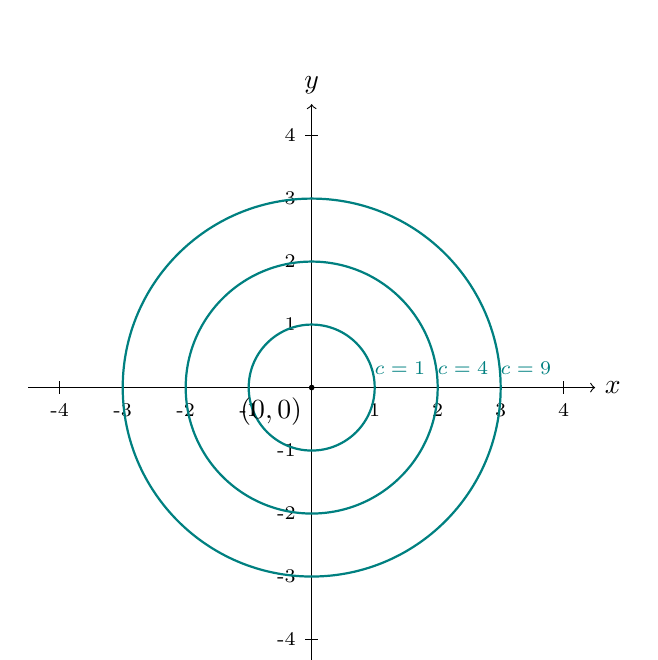
\begin{tikzpicture}[scale=0.8]
        \begin{scope}[shift={(0.5,0)}] % Desplaza todo a la derecha
            % Ejes
            \draw[->] (-4.5, 0) -- (4.5, 0) node[right] {$x$};
            \draw[->] (0, -4.5) -- (0, 4.5) node[above] {$y$};

            % Marcas y etiquetas en x
            \foreach \x in {-4,-3,-2,-1,1,2,3,4}
                \draw (\x,0.1) -- (\x,-0.1) node[below] {\scriptsize \x};

            % Marcas y etiquetas en y
            \foreach \y in {-4,-3,-2,-1,1,2,3,4}
                \draw (0.1,\y) -- (-0.1,\y) node[left] {\scriptsize \y};

            % Curvas de nivel: x^2 + y^2 = c
            \foreach \c in {1, 4, 9} {
                \draw[teal, thick] (0,0) circle ({sqrt(\c)});
                \node[teal, font=\scriptsize] at ({sqrt(\c)+0.4}, 0.3) {$c=\c$};
            }

            % Punto de referencia en el origen
            \filldraw[black] (0,0) circle (1pt) node[below left] {$(0,0)$};
        \end{scope}
    \end{tikzpicture}
    \caption{Curvas de nivel de \( z = x^2 + y^2 \): círculos para distintos valores de \( c \).}
\end{figure}


\subsection*{2a. Elipse: \(z=\dfrac{x^2}{a^2}+\dfrac{y^2}{b^2}\)}
\begin{itemize}
    \item \textbf{Curva de nivel:} \[
    \color{teal} \frac{x^2}{a^2}+\frac{y^2}{b^2}=c
    \]
    \item \textbf{Semiejes:} \(\color{teal} a\sqrt{c}\) en \(x\), \(\color{teal} b\sqrt{c}\) en \(y\); si \(c=0\), la curva se reduce al punto \(\color{teal} (0,0)\)
\end{itemize}



\subsection*{2b. Elipse: \(z=\dfrac{x^2}{a}+\dfrac{y^2}{b}\)}
\begin{itemize}
    \item \textbf{Curva de nivel:} \[
    \color{teal} \frac{x^2}{a}+\frac{y^2}{b}=c
    \]
    \item \textbf{Forma alternativa:} \[
    \color{teal} \frac{x^2}{ac} + \frac{y^2}{bc} = 1
    \]
    \item \textbf{Semiejes:} \(\color{teal} \sqrt{ac}\) en \(x\), \(\color{teal} \sqrt{bc}\) en \(y\); para \(c=0\), punto \(\color{teal} (0,0)\)
\end{itemize}






\begin{figure}[H]
    \centering
    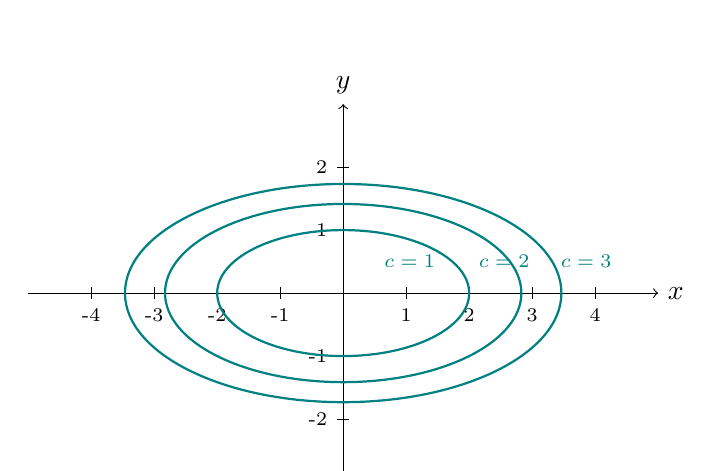
\begin{tikzpicture}[scale=0.8]
        \begin{scope}[shift={(0.5,0)}]

            % Parámetros
            \def\a{2} % a en el denominador de x^2
            \def\b{1} % b en el denominador de y^2

            % Ejes
            \draw[->] (-5, 0) -- (5, 0) node[right] {$x$};
            \draw[->] (0, -3) -- (0, 3) node[above] {$y$};

            % Marcas y etiquetas en x
            \foreach \x in {-4,-3,-2,-1,1,2,3,4}
                \draw (\x,0.1) -- (\x,-0.1) node[below] {\scriptsize \x};

            % Marcas y etiquetas en y
            \foreach \y in {-2,-1,1,2}
                \draw (0.1,\y) -- (-0.1,\y) node[left] {\scriptsize \y};

            % Curvas de nivel: elipses para c = 1, 2, 3
            \foreach \c/\col in {1/teal, 2/teal, 3/teal} {
                \pgfmathsetmacro{\rx}{\a*sqrt(\c)}
                \pgfmathsetmacro{\ry}{\b*sqrt(\c)}
                \draw[\col, thick] (0,0) ellipse [x radius=\rx, y radius=\ry];
            }

            % Leyenda manual
            \node[anchor=west, font=\scriptsize] at (0.5,0.5) {\color{teal} $c=1$};
            \node[anchor=west, font=\scriptsize] at (2,0.5) {\color{teal} $c=2$};
            \node[anchor=west, font=\scriptsize] at (3.3,0.5) {\color{teal} $c=3$};

        \end{scope}
    \end{tikzpicture}
    \caption{Curvas de nivel de \( z = \frac{x^2}{4} + \frac{y^2}{1} \)}
\end{figure}

% PONER A =4 y B=1
\subsection*{3. Hipérbola: \(z=axy\)}
\begin{itemize}
    \item \textbf{Curva de nivel:} \[
    \color{teal} y = \frac{c}{ax}
    \]
    \item \textbf{Casos:} Para \(\color{teal} c=0\), la curva es \(\color{teal} x=0 \cup y=0\), es decir, los ejes coordenados.
\end{itemize}

\begin{figure}[h]
    \centering
    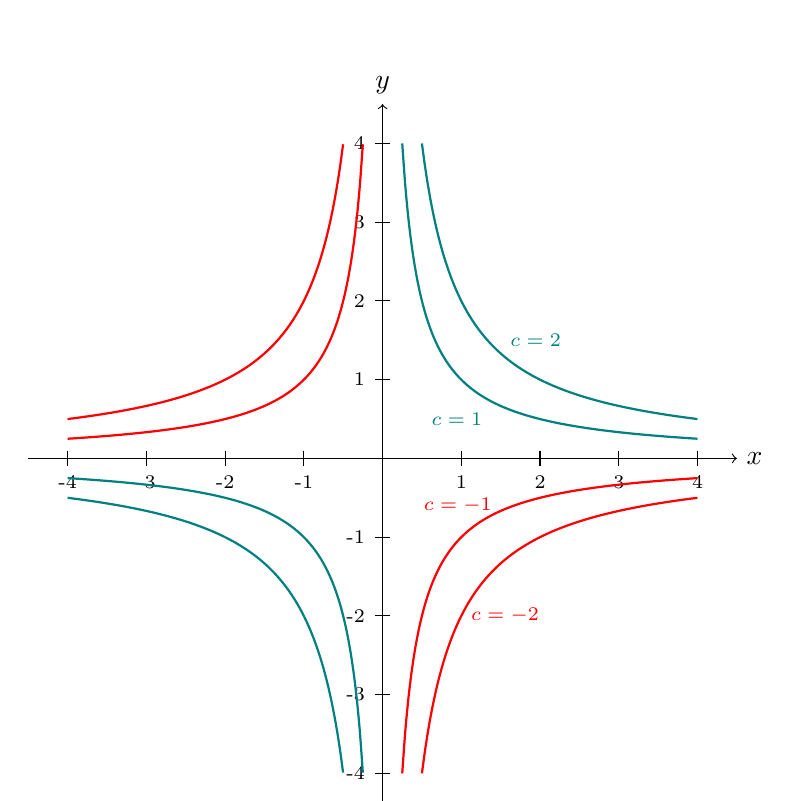
\begin{tikzpicture}[scale=1.0]
        \begin{scope}[shift={(0.5,0)}]
            % Parámetro a
            \def\a{1}
            
            % Ejes coordenados
            \draw[->] (-4.5,0) -- (4.5,0) node[right] {$x$};
            \draw[->] (0,-4.5) -- (0,4.5) node[above] {$y$};

            % Marcas en los ejes
            \foreach \x in {-4,-3,-2,-1,1,2,3,4}
                \draw (\x,0.1) -- (\x,-0.1) node[below] {\scriptsize \x};
            \foreach \y in {-4,-3,-2,-1,1,2,3,4}
                \draw (0.1,\y) -- (-0.1,\y) node[left] {\scriptsize \y};

            % Curvas de nivel positivas: c = 1 y c = 2 en teal
            \foreach \c in {1,2} {
                \pgfmathsetmacro{\d}{abs(\c)/4}
                \draw[domain=-4:-\d, smooth, variable=\x, thick, teal, samples=100]
                    plot ({\x}, {\c/(\a*\x)});
                \draw[domain=\d:4, smooth, variable=\x, thick, teal, samples=100]
                    plot ({\x}, {\c/(\a*\x)});
            }
            
            % Curvas de nivel negativas: c = -1 y c = -2 en red
            \foreach \c in {-1,-2} {
                \pgfmathsetmacro{\d}{abs(\c)/4}
                \draw[domain=-4:-\d, smooth, variable=\x, thick, red, samples=100]
                    plot ({\x}, {\c/(\a*\x)});
                \draw[domain=\d:4, smooth, variable=\x, thick, red, samples=100]
                    plot ({\x}, {\c/(\a*\x)});
            }
            
            % Ejemplos de labels libres (modificá las coordenadas según tu gusto):
             \node[anchor=west, font=\scriptsize, teal] at (0.5,0.5) {$c=1$};
             \node[anchor=west, font=\scriptsize, teal] at (1.5,1.5) {$c=2$};
             \node[anchor=west, font=\scriptsize, red] at (0.4,-0.6) {$c=-1$};
            \node[anchor=west, font=\scriptsize, red] at (1,-2) {$c=-2$};
            
        \end{scope}
    \end{tikzpicture}
    \caption{Curvas de nivel de \( z = axy \): hipérbolas \( y = \frac{c}{ax} \) }
\end{figure}


\subsection*{4. Plano: \(ax+by=cz\)}
\begin{itemize}
    \item \textbf{Forma explícita:} \[
    \color{teal} z=\frac{a}{c}x+\frac{b}{c}y
    \]
    \item \textbf{Curvas de nivel:} \[
    \color{teal} ax+by=ck
    \]
    que representan rectas paralelas para distintos valores de \(k\).
\end{itemize}

\begin{figure}[h]
    \centering
    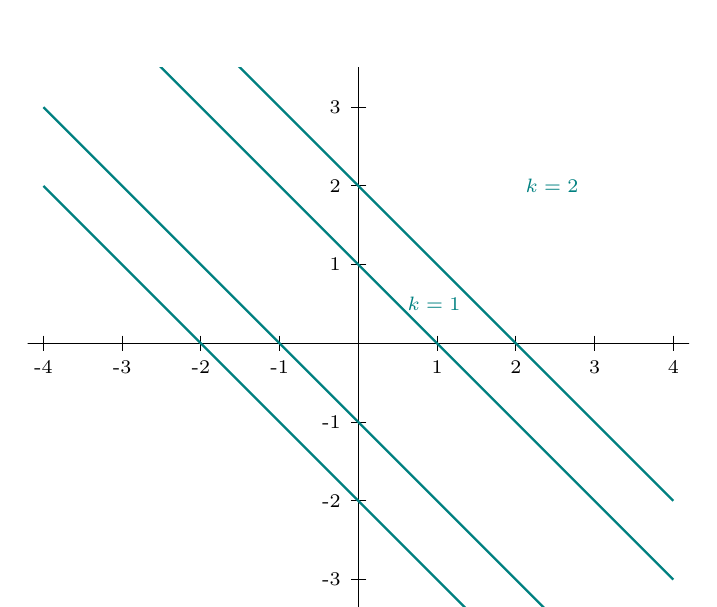
\begin{tikzpicture}[scale=1.0]
        \begin{scope}[shift={(0.5,0)}]
            % Limitar la región de dibujo a un rectángulo de x in [-4,4] y y in [-3,3]
            \clip (-4.2,-3.5) rectangle (4.2,3.5);
            
            % Parámetros: se pueden modificar según convenga
            \def\a{1}
            \def\b{1}
            \def\c{1}
            
            % Ejes coordenados
            \draw[->] (-4.5,0) -- (4.5,0) node[right] {$x$};
            \draw[->] (0,-4.5) -- (0,4.5) node[above] {$y$};

            % Marcas en los ejes
            \foreach \x in {-4,-3,-2,-1,1,2,3,4}
                \draw (\x,0.1) -- (\x,-0.1) node[below] {\scriptsize \x};
            \foreach \y in {-4,-3,-2,-1,1,2,3,4}
                \draw (0.1,\y) -- (-0.1,\y) node[left] {\scriptsize \y};

            % Curvas de nivel: ax+by = ck
            % Con a=1, b=1, c=1 se tiene x+y=k, es decir, y = k - x.
            \foreach \k in {-2,-1,1,2} {
                \draw[thick, teal, domain=-4:4, samples=100] 
                    plot (\x, {(\c*\k - \a*\x)/\b});
            }
            
            % Ejemplos de labels libres (descomentá y ajustá la posición según tu gusto):
            \node[anchor=west, font=\scriptsize, teal] at (0.5,0.5) {$k=1$};
            \node[anchor=west, font=\scriptsize, teal] at (2,2) {$k=2$};
            % \node[anchor=west, font=\scriptsize, teal] at (2,-1) {$k=-1$};
            % \node[anchor=west, font=\scriptsize, teal] at (2,-2) {$k=-2$};
            
        \end{scope}
    \end{tikzpicture}
    \caption{Curvas de nivel del plano \(ax+by=cz\): rectas paralelas \(ax+by=ck\) para distintos valores de \(k\),}
\end{figure}


\subsection*{5. Hipérbola: \(z = x^2 - y^2\)}
\begin{itemize}
    \item \textbf{Curva de nivel:} \[
    \color{teal} x^2 - y^2 = c
    \]
    \item \textbf{Casos:}
    \begin{itemize}
        \item \(\mathbf{c > 0}\): \[
        \color{teal} \frac{x^2}{c} - \frac{y^2}{c} = 1
        \]
        vértices en \(x = \pm\color{teal} \sqrt{c}\)

        \item \(\mathbf{c = 0}\): \[
        \color{teal} y = x \quad \text{y} \quad y = -x
        \]

        \item \(\mathbf{c < 0}\): \[
        \color{teal} \frac{y^2}{|c|} - \frac{x^2}{|c|} = 1
        \]
        vértices en \(y = \pm\color{teal} \sqrt{|c|}\)
    \end{itemize}
\end{itemize}


\begin{figure}[H]
    \centering
    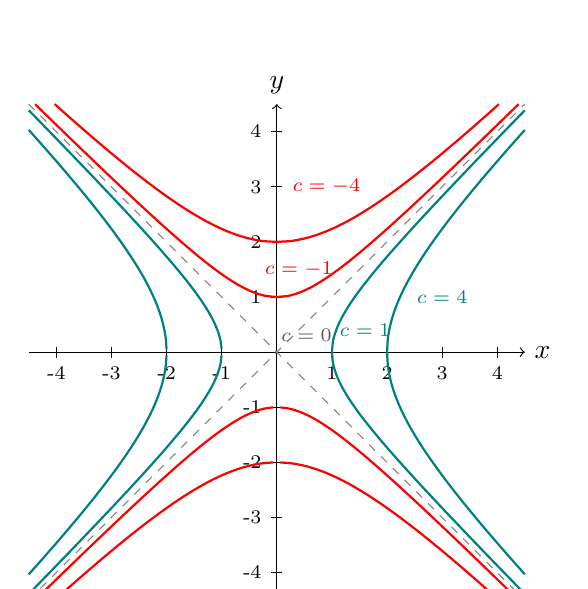
\begin{tikzpicture}[scale=0.7]
        \begin{scope}[shift={(0.5,0)}]
            % Axes
            \draw[->] (-4.5,0) -- (4.5,0) node[right] {$x$};
            \draw[->] (0,-4.5) -- (0,4.5) node[above] {$y$};

            % Ticks
            \foreach \x in {-4,-3,-2,-1,1,2,3,4}
                \draw (\x,0.1) -- (\x,-0.1) node[below] {\scriptsize \x};
            \foreach \y in {-4,-3,-2,-1,1,2,3,4}
                \draw (0.1,\y) -- (-0.1,\y) node[left] {\scriptsize \y};

            % c = 0 (asymptotes): y = x and y = -x
            \draw[dashed, gray] (-4.5,-4.5) -- (4.5,4.5);
            \draw[dashed, gray] (-4.5,4.5) -- (4.5,-4.5);
            \node[gray!70!black, font=\scriptsize, anchor=west] at (-0.1,0.3) {$c=0$};

            % Positive c: x^2 - y^2 = c (open along x)
            \foreach \c in {1,4} { % quitamos c=9
                \pgfmathsetmacro{\d}{sqrt(\c)}
                % upper branch
                \draw[domain=\d:4.5, samples=200, smooth, variable=\x, teal, thick]
                    plot (\x, {sqrt(\x*\x - \c)});
                \draw[domain=-4.5:-\d, samples=200, smooth, variable=\x, teal, thick]
                    plot (\x, {sqrt(\x*\x - \c)});
                % lower branch
                \draw[domain=\d:4.5, samples=200, smooth, variable=\x, teal, thick]
                    plot (\x, {-sqrt(\x*\x - \c)});
                \draw[domain=-4.5:-\d, samples=200, smooth, variable=\x, teal, thick]
                    plot (\x, {-sqrt(\x*\x - \c)});
            }

            % Negative c: x^2 - y^2 = -k  =>  y^2 - x^2 = k (open along y)
            \foreach \k in {1,4} { % quitamos k=9
                \pgfmathsetmacro{\d}{sqrt(\k)}
                % right/left branches for y >= d
                \draw[domain=\d:4.5, samples=200, smooth, variable=\y, red, thick]
                    plot ({ sqrt(\y*\y - \k)}, {\y});
                \draw[domain=\d:4.5, samples=200, smooth, variable=\y, red, thick]
                    plot ({-sqrt(\y*\y - \k)}, {\y});
                % right/left branches for y <= -d
                \draw[domain=-4.5:-\d, samples=200, smooth, variable=\y, red, thick]
                    plot ({ sqrt(\y*\y - \k)}, {\y});
                \draw[domain=-4.5:-\d, samples=200, smooth, variable=\y, red, thick]
                    plot ({-sqrt(\y*\y - \k)}, {\y});
            }

            % Example labels (tweak positions if desired)
            \node[teal, font=\scriptsize] at (1.6,0.4) {$c=1$};
            \node[teal, font=\scriptsize] at (3.0,1.0) {$c=4$};

            \node[red, font=\scriptsize] at (0.4,1.5) {$c=-1$};
            \node[red, font=\scriptsize] at (0.9,3.0) {$c=-4$};
        \end{scope}
    \end{tikzpicture}
    \caption{Curvas de nivel de \( z = x^2 - y^2 \): para \(c>0\) abren sobre el eje \(x\); para \(c<0\) (rojo) abren sobre el eje \(y\). El caso \(c=0\) son las rectas \(y=\pm x\) (grises, punteadas).}
\end{figure}





\newpage
\section{Curvas de nivel en Economía}

En esta sección se analiza la importancia de las {\color{teal}curvas de nivel} en el contexto económico, enfocándonos en su uso para representar y analizar funciones de producción y utilidad.

\begin{itemize}
    \item {\color{teal}Curvas de Nivel:} Representan conjuntos de puntos en los cuales una función de dos variables mantiene un mismo valor. En economía, se utilizan para identificar {\color{teal}combinaciones de insumos o bienes que generan un mismo nivel de producción o satisfacción}.
    \item {\color{teal}Isocuantas:} En funciones de producción, las curvas de nivel se denominan isocuantas, que muestran las {\color{teal}combinaciones de factores productivos que producen una cantidad constante de output}.
    \item {\color{teal}Curvas de Indiferencia:} En el análisis de la utilidad, las curvas de nivel se conocen como curvas de indiferencia y representan {\color{teal}combinaciones de bienes que proporcionan el mismo nivel de satisfacción al consumidor}.
\end{itemize}



\section*{Propiedades Deseables de las Curvas de Nivel en Economía}

Las curvas de nivel derivadas de funciones de utilidad deben exhibir ciertas propiedades para reflejar comportamientos económicos razonables. A continuación, se describen las características y la intuición económica asociada a cada una:

\subsection*{1. No se Cortan}
\begin{itemize}
    \item Intuición Económica: Cada curva de nivel representa un {\color{teal}nivel único de utilidad}. Si dos curvas se cruzaran, implicaría que una misma combinación de bienes podría proporcionar {\color{teal}dos niveles diferentes de satisfacción}, lo cual es inconsistente en el análisis de preferencias.
\end{itemize}

\subsection*{2. Pendiente Negativa}
\begin{itemize}
    \item Intuición Económica: Para mantener constante la utilidad, un aumento en la cantidad de un bien debe ir acompañado de una disminución en la cantidad del otro.
\end{itemize}

\subsection*{3. Monotonicidad}
\begin{itemize}
    \item Intuición Económica: La {\color{teal}monotonicidad} implica que al aumentar la cantidad de cualquiera de los bienes (mientras se mantiene la otra constante), la utilidad no disminuye. En la gráfica, esto se traduce en curvas que {\color{teal}crecen hacia arriba y a la derecha}, reflejando la preferencia por más cantidad de bienes.
\end{itemize}

\subsection*{4. Continuidad}
\begin{itemize}
    \item Intuición Económica: La {\color{teal}continuidad} asegura que pequeñas variaciones en las cantidades de bienes resultan en pequeños cambios en la utilidad. Esto permite predecir el comportamiento del consumidor sin {\color{teal}saltos abruptos} en sus niveles de satisfacción.
\end{itemize}

\subsection*{5. Convexidad al Origen}
\begin{itemize}
    \item Intuición Económica: A medida que se dispone de más de un bien, el consumidor está dispuesto a sacrificar cada vez menos del otro para obtener una unidad adicional del primero. Es una manifestación de la preferencia por {\color{teal}combinaciones balanceadas de bienes}, evitando consumir cantidades extremas de uno solo.
\end{itemize}

\section*{Recta Presupuestaria y Métodos de Graficación}

La {\color{teal}recta presupuestaria} representa las combinaciones de dos bienes que un consumidor puede adquirir gastando todo su ingreso, dados los precios de dichos bienes.

\subsection*{Método 1: Despejar una Variable en Función de la Otra}
Ecuación general de la restricción presupuestaria:
\begin{equation*}
{\color{teal}p_1 q_1 + p_2 q_2 = R}
\end{equation*}
Despejando \( q_2 \) en función de \( q_1 \):
\begin{equation*}
{\color{teal}q_2 = \frac{R}{p_2} - \frac{p_1}{p_2} q_1}
\end{equation*}
\begin{itemize}
    \item Intuición: La ecuación muestra que, a medida que aumenta la cantidad de \( q_1 \), la cantidad de \( q_2 \) debe disminuir para mantener constante el gasto total \( R \). La {\color{teal}pendiente} \( -\frac{p_1}{p_2} \) refleja la {\color{teal}tasa a la cual se puede intercambiar bienes}.
    \item Aplicación: Este método permite graficar la recta presupuestaria como una función lineal, facilitando el {\color{teal}análisis algebraico} de las decisiones del consumidor.
\end{itemize}

\subsection*{Método 2: Utilizar los Interceptos}
\begin{itemize}
    \item Intercepto en el eje \( q_1 \):
    \begin{equation*}
    {\color{teal}q_1 = \frac{R}{p_1}}
    \end{equation*}
    \item Intercepto en el eje \( q_2 \):
    \begin{equation*}
    {\color{teal}q_2 = \frac{R}{p_2}}
    \end{equation*}
\end{itemize}
\begin{itemize}
    \item Intuición: Estos interceptos representan las {\color{teal}cantidades máximas} de cada bien si el consumidor gasta todo su ingreso en uno solo.
    \item Aplicación: Conociendo ambos puntos, se traza la recta que los une. Esta gráfica ilustra de manera clara las {\color{teal}opciones de combinación} de bienes disponibles.
\end{itemize}

\section*{Curva de Costo para el Productor}

La {\color{teal}curva de isocosto} representa las combinaciones de insumos que se pueden adquirir para un {\color{teal}costo total fijo}:
\begin{equation*}
{\color{teal}w_1 x_1 + w_2 x_2 = C}
\end{equation*}
donde \(w_1\) y \(w_2\) son los precios de los insumos, \(x_1\) y \(x_2\) sus cantidades. 


\section*{Isoingreso}

La {\color{teal}línea de isoingreso} representa las combinaciones de productos o bienes que generan un {\color{teal}ingreso total constante}:
\begin{equation*}
{\color{teal}p_1 q_1 + p_2 q_2 = I}
\end{equation*}



\section*{Curvas de Indiferencia Cobb-Douglas}

Las {\color{teal}curvas de indiferencia} derivadas de una función de utilidad Cobb-Douglas representan combinaciones de bienes que otorgan un {\color{teal}nivel constante de utilidad}. Una forma general de esta función es:
\begin{equation*}
{\color{teal}U(x_1, x_2) = x_1^\alpha x_2^\beta}
\end{equation*}
donde \( \alpha, \beta > 0 \).

\subsection*{Graficando}
\begin{itemize}
    \item Despejar una Variable:
    \begin{equation*}
    {\color{teal}x_2 = \left( \frac{U_0}{x_1^\alpha} \right)^{\frac{1}{\beta}}}
    \end{equation*}
    o, equivalentemente,
    \begin{equation*}
    {\color{teal}x_2 = \frac{U^{1/\beta}}{x_1^{\alpha/\beta}}}
    \end{equation*}
    Esto permite graficar la curva de indiferencia para un nivel dado de utilidad \( U \), considerando distintos valores de \( x_1 \).

    \item Observaciones:
    \begin{itemize}
        \item Las curvas son {\color{teal}convexas al origen}, lo que refleja una {\color{teal}tasa marginal de sustitución decreciente}.
        \item {\color{teal}Nunca tocan los ejes}, ya que si \( x_1 = 0 \) o \( x_2 = 0 \), entonces la utilidad total es cero.
        \item Las curvas se ubican en el primer cuadrante, ya que se supone que el consumidor sólo considera {\color{teal}cantidades positivas de bienes}.
    \end{itemize}
\end{itemize}

Cada curva representa un {\color{teal}nivel fijo de utilidad}, y al aumentar dicho nivel, las curvas se desplazan hacia arriba y a la derecha, reflejando {\color{teal}preferencias monótonas}.

\vspace{0.5em}
{\color{teal}Nota:} {\color{teal}Las funciones de producción también suelen tener forma Cobb-Douglas}, en cuyo caso las curvas de nivel se denominan {\color{teal}isocuantas} y reflejan {\color{teal}combinaciones de factores productivos} que permiten obtener una misma cantidad de producto.





\newpage

\section{Optimización con curvas de nivel}


\section*{Método de Igualación de Derivadas para la Optimización con Restricción}

Supongamos que queremos optimizar (maximizar o minimizar) una función objetivo \(F(x,y)\) sujeta a una restricción \(G(x,y)=C\). La idea es asumir que, en el punto óptimo, el valor de la función objetivo es constante y, de esta forma, expresar una de las variables en función de la otra a partir de ambas ecuaciones (la función objetivo y la restricción). Luego, derivamos cada despeje respecto a la otra variable, igualamos las derivadas y, a partir de esa igualdad, {\color{teal}obtenemos una relación entre \(x\) y \(y\) que, al sustituirla en la restricción, permite hallar la solución óptima.}

El procedimiento se resume en los siguientes pasos:
\begin{enumerate}
    \item \textbf{\color{teal}Fijar el nivel óptimo:}  
    Se asume que en el óptimo la función objetivo alcanza un valor constante, digamos \(F(x,y)=K\).  

    \item \textbf{\color{teal}Despejar \(x\) (o \(y\)) en función de \(y\) (o \(x\)):}  
    Se resuelve la ecuación \(F(x,y)=K\) para obtener una expresión del tipo
    \[
    x = f(y),
    \]
    y se despeja la misma variable a partir de la restricción:
    \[
    x = g(y) \quad \text{(obtenido de } G(x,y)=C\text{)}.
    \]
    
    \item \textbf{\color{teal}Derivar respecto a la otra variable:}  
    Se derivan ambas expresiones con respecto a \(y\). Así se obtienen:
    \[
    \frac{dx}{dy}\Big|_{\text{objetivo}} = f'(y) \quad \text{y} \quad \frac{dx}{dy}\Big|_{\text{restricción}} = g'(y).
    \]
    
    \item \textbf{\color{teal}Igualar las derivadas:}  
    En el punto óptimo ambas curvas son tangentes, por lo que sus pendientes deben coincidir. Esto implica:
    \[
    f'(y)=g'(y).
    \]
    Esta igualdad permite despejar una relación entre \(x\) e \(y\) (o encontrar el valor de \(y\)).
    
    \item \textbf{\color{teal}Realizar el proceso con el otro despeje:}  
    De manera análoga, se despeja \(y\) en función de \(x\) tanto a partir de la función objetivo como de la restricción:
    \[
    y = h(x) \quad \text{y} \quad y = k(x),
    \]
    y se derivan ambas expresiones respecto a \(x\):
    \[
    \frac{dy}{dx}\Big|_{\text{objetivo}} = h'(x) \quad \text{y} \quad \frac{dy}{dx}\Big|_{\text{restricción}} = k'(x).
    \]
    Igualando estas derivadas se obtiene otra relación entre \(x\) e \(y\). Esta segunda igualdad, junto con la anterior, permite eliminar el parámetro \(K\) (el valor fijo de la función objetivo) y obtener una relación única entre \(x\) e \(y\).

    \item \textbf{\color{teal}Sustituir en la restricción:}  
    Con la relación obtenida se reemplaza en la restricción original \(G(x,y)=C\) para calcular el valor óptimo de una de las variables y, a partir de allí, el otro.
\end{enumerate}


\section*{Ejemplo: Optimización de \(f(x,y)=x^2y\) sujeta a \(5x+2y=100\)}

Sea la función objetivo
\[
f(x,y)=x^2y,
\]
y la restricción
\[
5x+2y=100.
\]
En el óptimo se asume que \(f(x,y)=K\) es constante.

\subsection*{Despejar \(x\) en función de \(y\)}

\begin{itemize}
    \item \textbf{Desde la función objetivo:}  
    Partiendo de
    \[
    x^2y=K,
    \]
    despejamos \(x\) (tomando la rama positiva\footnote{Tomar la solución positiva del despeje es algo que comúnmente se hace en ejemplos económicos ya que las variables suelen tener interpretación de bienes o precios, los cuales nunca podrían ser negativos.}):
    \[
    x=\sqrt{\frac{K}{y}}=\sqrt{K}\;y^{-1/2}.
    \]
    
    \item \textbf{Desde la restricción:}  
    De
    \[
    5x+2y=100,
    \]
    se obtiene:
    \[
    x=\frac{100-2y}{5}.
    \]
    
    \item \textbf{Derivar respecto a \(y\):}
    \begin{itemize}
        \item Para la función objetivo:
        \[
        \frac{dx}{dy}=-\frac{1}{2}\sqrt{K}\;y^{-3/2}.
        \]
        \item Para la restricción:
        \[
        \frac{dx}{dy}=-\frac{2}{5}.
        \]
    \end{itemize}
    
    \item \textbf{Igualar las derivadas:}  
    En el óptimo se tiene:
    \[
    -\frac{1}{2}\sqrt{K}\;y^{-3/2}=-\frac{2}{5}.
    \]
    Cancelando el signo negativo y despejando \(\sqrt{K}\):
    \[
    \frac{1}{2}\sqrt{K}\;y^{-3/2}=\frac{2}{5} \quad\Longrightarrow\quad \sqrt{K}=\frac{4}{5}\;y^{3/2}.
    \]
    Elevando al cuadrado se obtiene:
    \[
    K=\frac{16}{25}\;y^3.
    \]
\end{itemize}

\subsection*{Despejar \(y\) en función de \(x\)}

\begin{itemize}
    \item \textbf{Desde la función objetivo:}  
    Partiendo de
    \[
    x^2y=K,
    \]
    despejamos \(y\):
    \[
    y=\frac{K}{x^2}.
    \]
    
    \item \textbf{Desde la restricción:}  
    De
    \[
    5x+2y=100,
    \]
    despejamos \(y\):
    \[
    y=\frac{100-5x}{2}.
    \]
    
    \item \textbf{Derivar respecto a \(x\):}
    \begin{itemize}
        \item Para la función objetivo:
        \[
        y=K\,x^{-2}\quad\Longrightarrow\quad \frac{dy}{dx}=-2K\,x^{-3}.
        \]
        \item Para la restricción:
        \[
        \frac{dy}{dx}=-\frac{5}{2}.
        \]
    \end{itemize}
    
    \item \textbf{Igualar las derivadas:}  
    Se igualan:
    \[
    -2K\,x^{-3}=-\frac{5}{2}.
    \]
    Cancelando el signo negativo y despejando \(K\):
    \[
    2K\,x^{-3}=\frac{5}{2} \quad\Longrightarrow\quad K=\frac{5}{4}\,x^3.
    \]
\end{itemize}

\subsection*{Igualación de los valores de \(K\) y obtención de la relación entre \(x\) e \(y\)}

De los dos procesos obtenemos:
\[
K=\frac{16}{25}\,y^3 \quad \text{y} \quad K=\frac{5}{4}\,x^3.
\]
Igualando:
\[
\frac{16}{25}\,y^3=\frac{5}{4}\,x^3.
\]
Multiplicamos ambos lados por \(100\) (o directamente despejamos) para simplificar:
\[
\frac{16\cdot 4}{25\cdot 4}\,y^3=\frac{5\cdot 25}{4\cdot 25}\,x^3 \quad\Longrightarrow\quad \frac{64}{100}\,y^3=\frac{125}{100}\,x^3,
\]
lo que simplifica a:
\[
64\,y^3=125\,x^3.
\]
Dividiendo ambos lados por \(x^3\):
\[
\left(\frac{y}{x}\right)^3=\frac{125}{64},
\]
y, al tomar la raíz cúbica:
\[
\color{teal}\frac{y}{x}=\frac{5}{4} \quad\Longrightarrow\quad y=\frac{5}{4}\,x.
\]

\subsection*{Sustitución en la restricción para hallar \(x\) y \(y\)}

Sustituyendo \(y=\frac{5}{4}\,x\) en la restricción
\[
5x+2y=100,
\]
se tiene:
\[
5x+2\left(\frac{5}{4}\,x\right)=5x+\frac{10}{4}\,x=5x+\frac{5}{2}\,x=\frac{10x+5x}{2}=\frac{15x}{2}=100.
\]
Despejamos \(x\):
\[
x=\frac{100\cdot 2}{15}=\frac{200}{15}=\color{teal}\frac{40}{3}.
\]
Luego, \(y\) es:
\[
y=\frac{5}{4}\,x=\frac{5}{4}\cdot\frac{40}{3}=\frac{200}{12}=\color{teal}\frac{50}{3}.
\]

\subsection*{Valor óptimo de la función}

Finalmente, el valor óptimo de la función es:
\[
f\left(\frac{40}{3},\frac{50}{3}\right)=\left(\frac{40}{3}\right)^2\cdot\frac{50}{3}=\frac{1600}{9}\cdot\frac{50}{3}=\color{teal}\frac{80000}{27}.
\]

\subsection*{Resumen del Método}

\begin{enumerate}
    \item Se despeja \(x\) en función de \(y\) (y viceversa) a partir de la función objetivo \(x^2y=K\) y la restricción \(5x+2y=100\).
    \item Se derivan ambas expresiones con respecto a la variable correspondiente y se igualan, obteniéndose dos relaciones que involucran \(K\).
    \item Se igualan los valores de \(K\) obtenidos en ambos procesos para eliminar el parámetro \(K\) y obtener una relación única entre \(x\) e \(y\).
    \item Finalmente, se sustituye esta relación en la restricción para determinar los valores óptimos de \(x\) y \(y\).
\end{enumerate}



\section*{Ejemplo: Minimización de \(C = 3x_1 + 6x_2 + 180\) sujeta a \(x_1 x_2 = 2\)}

Se desea minimizar
\[
C = 3x_1 + 6x_2 + 180,
\]
sujeto a la restricción
\[
x_1 x_2 = 2.
\]
Fijamos un nivel constante para la función objetivo
\[
3x_1 + 6x_2 +180 = K,
\]

\subsection*{Paso 1: Derivación de la Función Objetivo}
Despejamos \(x_2\) en función de \(x_1\):
\[
x_2 = \frac{K - 180 - 3x_1}{6}.
\]
Al derivar con respecto a \(x_1\) se obtiene:
\[
\frac{dx_2}{dx_1} = -\frac{3}{6} = -\frac{1}{2}.
\]
Nótese que la derivada no depende de \(K\) (la constante desaparece).

\subsection*{Paso 2: Derivación de la Restricción}
A partir de la restricción
\[
x_1 x_2 = 2,
\]
despejamos \(x_2\):
\[
x_2 = \frac{2}{x_1}.
\]
Derivamos respecto a \(x_1\) se obtiene:
\[
\frac{dx_2}{dx_1} = -\frac{2}{x_1^2}.
\]

\subsection*{Paso 3: Igualar las Derivadas}
En el punto de tangencia entre la curva de nivel de la función objetivo y la curva de la restricción, sus pendientes deben ser iguales. Es decir:
\[\color{teal}
-\frac{1}{2} = -\frac{2}{x_1^2}.
\]
Cancelando el signo negativo y resolviendo:
\[\color{teal}
\frac{1}{2} = \frac{2}{x_1^2} \quad\Longrightarrow\quad x_1^2 = 4 \quad\Longrightarrow\quad x_1 = 2,
\]
(considerando \(x_1>0\)).

\subsection*{Paso 4: Determinar \(x_2\) y el Costo Óptimo}
Sustituyendo \(x_1=2\) en la restricción:
\[\color{teal}
x_2 = \frac{2}{2} = 1.
\]
Por tanto, el costo mínimo es:
\[
\color{teal}C_{\min} = 3(2) + 6(1) + 180 = 6 + 6 + 180 = 192.
\]



\section*{Método de Sustitución para la Optimización con Restricción}

Supongamos que queremos optimizar (maximizar o minimizar) una función objetivo \(F(x,y)\) sujeta a una restricción \(G(x,y)=C\). Este método consiste en despejar de la restricción una variable, sustituir esa expresión en la función objetivo para \textbf{\color{teal}reducir el problema a una única variable}, derivar respecto a esa variable, igualar a cero y, finalmente, resolver para encontrar la solución óptima.

El procedimiento se resume en los siguientes pasos:
\begin{enumerate}
    \item \textbf{\color{teal}Resolver la restricción:}  
    Dada la restricción
    \[
    G(x,y)=C,
    \]
    se despeja una de las variables. Por ejemplo, si despejamos \(y\) obtenemos:
    \[
    y = g(x).
    \]
    
    \item \textbf{\color{teal}Sustituir en la función objetivo:}  
    Se inserta \(y = g(x)\) en la función objetivo \(F(x,y)\) para obtener una función de una sola variable:
    \[
    f(x) = F(x, g(x)).
    \]
    
    \item \textbf{\color{teal}Derivar e igualar a cero:}  
    Se deriva la función \(f(x)\) respecto a \(x\) y se impone la condición de primer orden:
    \[
    \frac{df(x)}{dx} = 0.
    \]
    Esta ecuación se resuelve para hallar el valor óptimo \(x^*\).
    
    \item \textbf{\color{teal}Determinar la otra variable:}  
    Finalmente, se sustituye \(x^*\) en la expresión \(y = g(x)\) para obtener \(y^*\).
\end{enumerate}

Este método reduce el problema original de dos variables a uno de una sola variable, simplificando el proceso de optimización.



\section*{Ejemplo: Optimización de \(f(x,y)=x^2y\) sujeta a \(5x+2y=100\) (Método de Sustitución)}

Sea la función objetivo
\[
f(x,y)=x^2y,
\]
y la restricción
\[
5x+2y=100.
\]
El método de sustitución consiste en despejar una variable de la restricción, insertar esa expresión en la función objetivo para obtener una función de una sola variable, derivar respecto a dicha variable, igualar a cero y finalmente despejar.

\subsection*{Paso 1: Resolver la restricción}
De la ecuación
\[
5x+2y=100,
\]
despejamos \(y\):
\[\color{teal}
y=\frac{100-5x}{2}.
\]

\subsection*{Paso 2: Sustituir en la función objetivo}
Insertamos la expresión de \(y\) en \(f(x,y)=x^2y\):
\[
f(x)=x^2\left({\color{teal}\frac{100-5x}{2}}\right)=\frac{1}{2}\left(100x^2-5x^3\right).
\]

\subsection*{Paso 3: Derivar e igualar a cero}
Derivamos \(f(x)\) respecto a \(x\):
\[
f'(x)=\frac{1}{2}\left(200x-15x^2\right)=100x-\frac{15}{2}x^2.
\]
Para hallar el óptimo, igualamos la derivada a cero:
\[
100x-\frac{15}{2}x^2=0.
\]
Factorizamos \(x\):
\[
x\left(100-\frac{15}{2}x\right)=0.
\]
Se obtienen dos soluciones: \(x=0\) (solución trivial) y
\[
100-\frac{15}{2}x=0 \quad\Longrightarrow\quad x=\frac{200}{15}=\frac{40}{3}.
\]
Descartamos \(x=0\) y tomamos \(\color{teal}x^*=\frac{40}{3}\).

\subsection*{Paso 4: Determinar \(y\)}
Sustituyendo \(x^*=\frac{40}{3}\) en la expresión de \(y\):
\[\color{teal}
y^*=\frac{100-5\left(\frac{40}{3}\right)}{2}=\frac{100-\frac{200}{3}}{2}=\frac{\frac{300-200}{3}}{2}=\frac{\frac{100}{3}}{2}=\frac{50}{3}.
\]

\subsection*{Paso 5: Valor óptimo de la función}
El valor óptimo de la función es:
\[\color{teal}
f\left(\frac{40}{3},\frac{50}{3}\right)=\left(\frac{40}{3}\right)^2\cdot\frac{50}{3}=\frac{80000}{27}.
\]

\subsection*{Resumen del Método de Sustitución}
\begin{enumerate}
    \item Se despeja una variable de la restricción, en este caso \(y=\frac{100-5x}{2}\).
    \item Se sustituye en la función objetivo para obtener \(f(x)=\frac{1}{2}(100x^2-5x^3)\).
    \item Se deriva \(f(x)\) respecto a \(x\) y se iguala a cero para encontrar el valor óptimo \(x^*\).
    \item Se utiliza \(x^*\) en la expresión de \(y\) para determinar \(y^*\).
    \item Se evalúa la función objetivo en \((x^*,y^*)\) para obtener el valor óptimo.
\end{enumerate}




\section*{Ejemplo: Minimización de \(C = 3x_1 + 6x_2 + 180\) sujeta a \(x_1 x_2 = 2\) (Método de Sustitución)}

Se desea minimizar
\[
C = 3x_1 + 6x_2 + 180,
\]
sujeto a la restricción
\[
x_1 x_2 = 2.
\]


\subsection*{Paso 1: Despejar una variable de la restricción}

A partir de la restricción \(x_1 x_2 = 2\), despejamos \(x_2\):
\[
x_2 = \frac{2}{x_1}.
\]

\subsection*{Paso 2: Sustituir en la función objetivo}

Sustituimos la expresión de \(x_2\) en la función objetivo simplificada:
\[
\widetilde{C}(x_1) = 3x_1 + 6\left({\color{teal}\frac{2}{x_1}}\right) +180 = 3x_1 + \frac{12}{x_1} +180
\]

\subsection*{Paso 3: Derivar e igualar a cero}

Derivamos la función \(\widetilde{C}(x_1)\) respecto a \(x_1\):
\[
\frac{d\widetilde{C}}{dx_1} = 3 - \frac{12}{x_1^2}.
\]
Para hallar el mínimo, igualamos la derivada a cero:
\[
3 - \frac{12}{x_1^2} = 0.
\]
Resolviendo:
\[
\frac{12}{x_1^2} = 3 \quad \Longrightarrow \quad x_1^2 = \frac{12}{3} = 4,
\]
por lo que, considerando \(x_1 > 0\),
\[\color{teal}
x_1^* = 2.
\]

\subsection*{Paso 4: Determinar \(x_2\) y el costo óptimo}

Sustituyendo \(x_1 = 2\) en la expresión de \(x_2\):
\[\color{teal}
x_2^* = \frac{2}{2} = 1.
\]
El costo mínimo es, entonces:
\[\color{teal}
C_{\min} = 3(2) + 6(1) + 180 = 6 + 6 + 180 = 192.
\]

\subsection*{Resumen del Método de Sustitución}
\begin{enumerate}
    \item Se despeja \(x_2\) de la restricción \(x_1 x_2 = 2\): \(x_2 = \frac{2}{x_1}\).
    \item Se sustituye en la función objetivo simplificada \(\widetilde{C} = 3x_1 + 6x_2\) para obtener
    \[
    \widetilde{C}(x_1) = 3x_1 + \frac{12}{x_1}.
    \]
    \item Se deriva respecto a \(x_1\) e iguala la derivada a cero para hallar \(x_1^*\).
    \item Se determina \(x_2^*\) usando la expresión de la restricción y se evalúa \(C\).
\end{enumerate}

\section*{Soluciones de Esquina}

Es importante notar que el método de sustitución (o igualación de derivadas) asume que la solución óptima es interior, es decir, que la curva de nivel de la función objetivo es tangente a la restricción. Este método no es aplicable cuando el óptimo se alcanza en una solución de esquina.

\medskip

\textbf{Ejemplo breve:}  
Considera la maximización de
\[
f(x,y)=x+y,
\]
sujeta a las restricciones
\[
\begin{cases}
x+y\leq 1,\\[1mm]
x\geq 0,\quad y\geq 0.
\end{cases}
\]
En este problema, el óptimo se alcanza en las esquinas \((0,1)\) o \((1,0)\), donde no existe tangencia entre la curva de nivel y la frontera. Por ello, métodos basados en la igualación de derivadas no serían adecuados en este caso.




\newpage


\section{Continuidad}


En esta sección vamos a repasar rápidamente los {\color{teal}límites y la continuidad en una variable} y extenderemos las ideas al caso de {\color{teal}dos variables} (o más). 

\section*{Repaso: límites y continuidad en una variable}
Sea \(f\colon I\subseteq \mathbb{R}\to\mathbb{R}\) y \(a\in I\).
\begin{itemize}

  \item \textbf{{\color{teal}Continuidad en \(a\)}}:
  \[\color{teal}
    f \text{ es continua en } a
    \;\Longleftrightarrow\;
    \lim_{x\to a} f(x)=f(a).
  \]
\end{itemize}
Esta definición engloba 3 condiciones:
\begin{itemize}
    \item {\color{teal} La función existe en el punto $a$ }
    \item{ \color{teal}El límite de la función existe cuando $x\to a$}
    \item {\color{teal}El valor de la función en el punto y el límite coinciden.}
\end{itemize}



\subsection*{Ejemplos}

Sea
\[
f(x)=(x+1)^2.
\]
Tomemos \(a=1\). Verificamos continuidad en \(a\) con las tres condiciones:

\begin{itemize}
  \item {\color{teal}Existencia de \(f(1)\):} \(f(1)=1^{2}+2\cdot1+1=4\).
  \item {\color{teal}Existencia del límite:}
  \[
    \lim_{x\to 1} f(x)=\lim_{x\to 1}(x^{2}+2x+1)
    =1^{2}+2\cdot1+1=4.
  \]
  \item {\color{teal}Coincidencia límite–valor:} \(\displaystyle \lim_{x\to1}f(x)=4=f(1)\).
\end{itemize}

Por lo tanto, {\color{teal}\(f\) es continua en \(x=1\)} (de hecho, en todo \(\mathbb R\) por ser polinómica).  \\
\\
Veamos otro ejemplo. Definimos
\[
g(x)=
\begin{cases}
\dfrac{x^{2}-1}{x-1}, & x\neq 1,\\[6pt]
0, & x=1.
\end{cases}
\]
Observemos que para \(x\neq1\),
\[
\frac{x^{2}-1}{x-1}=\frac{(x-1)(x+1)}{x-1}=x+1,
\]
luego
\[
\lim_{x\to1}g(x)=\lim_{x\to1}(x+1)=2.
\]
Sin embargo, \(g(1)=0\). Entonces:

\begin{itemize}
  \item {\color{teal}Existe \(g(1)\):} \(g(1)=0\).
  \item {\color{teal}Existe el límite:} \(\displaystyle \lim_{x\to1}g(x)=2\).
  \item {\color{teal}No coinciden:} \(2\neq 0\).
\end{itemize}

Por lo tanto, {\color{teal}\(g\) es discontinua en \(x=1\)} (discontinuidad \emph{evitable}, ya que si redefiniéramos \(g(1)=2\) se volvería continua).

Veamos un último ejemplo. Sea
\[
f(x)=\frac{1}{x-2}.
\]
Analicemos en \(a=2\).

\begin{itemize}
  \item {\color{teal}Existencia de \(f(2)\):} \(f(2)\) no está definida (el denominador se anula).
  \item {\color{teal}Comportamiento del límite:}
  \[
    \lim_{x\to 2^-}\frac{1}{x-2}=-\infty,
    \qquad
    \lim_{x\to 2^+}\frac{1}{x-2}=+\infty.
  \]
  Por lo tanto, \(\displaystyle \lim_{x\to 2}f(x)\) no existe como número finito.
\end{itemize}

En consecuencia, {\color{teal}\(f\) presenta una discontinuidad \emph{infinita} en \(x=2\)} y la recta \(x=2\) es una \emph{asíntota vertical}.


\section*{Límites y continuidad en dos variables}

Sea \(f\colon D\subseteq\mathbb{R}^2\to\mathbb{R}\) y \(a=(a_1,a_2)\in D\).

\begin{itemize}
  \item \textbf{{\color{teal}Continuidad en \(a\)}}:
  \[
    \color{teal}
    f \text{ es continua en } a
    \;\Longleftrightarrow\;
    \lim_{(x,y)\to(a_1,a_2)} f(x,y)=f(a_1,a_2).
  \]
\end{itemize}

Como en una variable, esta condición resume tres hechos:
\begin{itemize}
  \item {\color{teal}La función está definida en \(a\):} \(f(a_1,a_2)\) existe.
  \item {\color{teal}El límite existe al acercarse a \(a\):}
  \(\displaystyle \lim_{(x,y)\to(a_1,a_2)} f(x,y)\) existe (es único).
  \item {\color{teal}Coinciden límite y valor:}
  \(\displaystyle \lim_{(x,y)\to(a_1,a_2)} f(x,y)=f(a_1,a_2)\).
\end{itemize}


\subsection*{Ejemplos}

Sea
\[
f(x,y)=x^{2}+2xy+3y^{2}.
\]
Verifiquemos primero la continuidad en el punto específico \(a=(1,2)\).

\begin{itemize}
  \item {\color{teal}Existencia de \(f(a)\):} 
  \[
  f(1,2)=1^{2}+2\cdot1\cdot2+3\cdot2^{2}=1+4+12=17.
  \]
  \item {\color{teal}Existencia del límite y coincidencia con el valor:}
  Como \(f\) es un polinomio (suma y producto de funciones continuas),
  \[
  \lim_{(x,y)\to(1,2)}f(x,y)
  = f(1,2)=17.
  \]
\end{itemize}
Por lo tanto, {\color{teal}\(f\) es continua en \((1,2)\)}.

Además, como \(f\) es polinómica en \(x\) y \(y\), es {\color{teal}continua en todo \(\mathbb{R}^{2}\)}; es decir, para cualquier \(a=(a_1,a_2)\),
\[
\lim_{(x,y)\to(a_1,a_2)} f(x,y)=f(a_1,a_2).
\]
\\
Veamos otro caso, definimos
\[
g(x,y)=
\begin{cases}
1, & (x,y)\neq(0,0),\\[4pt]
0, & (x,y)=(0,0).
\end{cases}
\]
Al acercarse a \((0,0)\), se tiene
\(\displaystyle \lim_{(x,y)\to(0,0)} g(x,y)=1\),
pero \(g(0,0)=0\).
{\color{teal}Por lo tanto, \(\displaystyle \lim_{(x,y)\to(0,0)} g(x,y)\neq g(0,0)\) y \(g\) es \emph{discontinua} en \((0,0)\).}

Un último ejemplo. Sea
\[
h(x,y)=
\begin{cases}
\dfrac{xy}{x^{2}+y^{2}}, & (x,y)\neq(0,0),\\[8pt]
0, & (x,y)=(0,0).
\end{cases}
\]
Cuando tenemos una sola variable independiente, uno puede acercarse al punto por izquierda y por derecha, pero al trabajar con dos variables independientes uno puede acercarse al punto de diferentes maneras, como por ejemplo a través de una relación lineal entre x e y. Considerando caminos rectos \(y=mx\).
\[
h(x,mx)=\frac{x\,(mx)}{x^{2}+m^{2}x^{2}}
= \frac{m}{1+m^{2}},
\]
cuyo límite cuando \(x\to0\) \emph{depende} de \(m\).
{\color{teal}Por ejemplo, por \(y=x\) el límite vale \(\tfrac{1}{2}\), mientras que por \(y=-x\) vale \(-\tfrac{1}{2}\).
Luego \(\displaystyle \lim_{(x,y)\to(0,0)} h(x,y)\) no existe y \(h\) es \emph{discontinua} en \((0,0)\).}


\newpage


\section{Derivadas parciales}





\section*{Derivada para funciones de una variable}

Para funciones de una variable la derivada relaciona el incremento de la función con el incremento de la variable independiente (cociente incremental) cuando el incremento de \(x\) tiende a cero

\[
f'(x_{0}) = \lim_{h\to0}\frac{f(x_{0}+h)-f(x_{0})}{h}
\]

Gráficamente:
\begin{center}
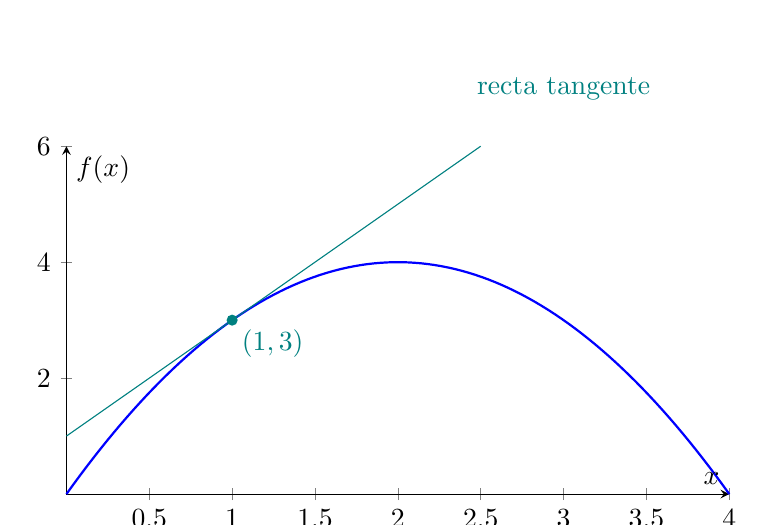
\begin{tikzpicture}
  \begin{axis}[
    width=10cm, height=6cm,
    axis lines=middle,
    xlabel=$x$, ylabel={$f(x)$},
    domain=0:4, samples=100,
    ymin=0, ymax=6,
    clip=false
  ]
    % Parábola cóncava hacia abajo con vértice en (2,4)
    \addplot[thick,blue] {-(x-2)^2 + 4};
    % Punto de tangencia en la rama creciente (x0=1)
    \coordinate (P) at (axis cs:1,3);
    \fill[teal] (P) circle (2pt) node[below right] {$(1,3)$};
    % Recta tangente con pendiente 2: y = 2(x-1) + 3
    \addplot[teal,domain=0:2.5] {2*(x-1) + 3};
    \node[teal] at (axis cs:3,7) {recta tangente};
  \end{axis}
\end{tikzpicture}
\end{center}
La función representada es:
\[
f(x) = -\,(x-2)^{2} + 4
\]
En el punto \((1,3)\), la pendiente de la recta tangente es precisamente la derivada de \(f\) respecto a \(x\):
\[
\color{teal}
\left.\frac{df}{dx}\right|_{x=1} = 2
\]
Como esta pendiente es positiva, la función en ese punto está aumentando.




\section*{Derivadas parciales}

Para una función de dos variables debemos considerar el incremento de la función \(z\) asociada a cambios en las variables independientes \(x\) e \(y\). Para ello, permitimos la variación de una variable manteniendo la otra constante.


Dada la función \(z = f(x,y)\), se define la derivada parcial de \(f\) con respecto a \(x\) en el punto \((x_{0},y_{0})\) como el valor del siguiente límite, si existe y es finito:

\[ \color{teal}
\frac{\partial f}{\partial x}(x_{0},y_{0})
=
\lim_{h\to0}
\frac{f(x_{0}+h,\,y_{0}) - f(x_{0},y_{0})}{h}
\]



Del mismo modo, se define la derivada parcial de \(f\) con respecto a \(y\) en el punto \((x_{0},y_{0})\) como el siguiente límite, si existe y es finito:

\[ \color{teal}
\frac{\partial f}{\partial y}(x_{0},y_{0})
=
\lim_{h\to0}
\frac{f(x_{0},\,y_{0}+h) - f(x_{0},y_{0})}{h}
\]
\paragraph*{Intuición:}

Básicamente consideramos un pequeño incremento \(h\) (que luego hacemos tender a cero) en una sola variable —\(x\) o \(y\)— mientras la otra permanece fija. A ese desplazamiento le restamos el valor original de la función para medir cuánto ha cambiado \(f\) al pasar del punto viejo al nuevo, y dividimos por la distancia \(h\) recorrida. De este modo obtenemos la variación de \(f\) por unidad de desplazamiento en esa dirección, que es precisamente la derivada parcial en ese punto.  



\subsection*{Derivadas parciales en \(\mathbb{R}^n\)}
Para generalizar lo anterior podemos pasar a $n$ variables:
Sea \(f\colon U\subseteq\mathbb{R}^n\to\mathbb{R}\) y sea \(a=(a_1,\dots,a_n)\in U\). Para cada \(i=1,\dots,n\), la derivada parcial de \(f\) con respecto a la variable \(x_i\) en el punto \(a\) se define como

\[
\color{teal}
\frac{\partial f}{\partial x_i}(a)
=
\lim_{h\to0}
\frac{f(a_1,\dots,a_{i-1},\,a_i+h,\,a_{i+1},\dots,a_n) \;-\; f(a_1,\dots,a_n)}{h}
\]


\subsection*{Ejemplo}

Sea la función  
\[
f(x,y)=x^{2}y + 3\,x\,y^{2}
\]

\subsubsection*{Por definición}
\[
\frac{\partial f}{\partial x}(1,2)
=
\lim_{h\to0}
\frac{f(1+h,2)-f(1,2)}{h}
\]
Calculamos
\[
f(1+h,2)
=2(1+h)^{2} + 12(1+h)
=2 + 4h + 2h^{2} + 12 + 12h
=14 + 16h + 2h^{2}
\quad
f(1,2)=14
\]
Luego
\[
\frac{f(1+h,2)-f(1,2)}{h}
=\frac{16h+2h^{2}}{h}
=16+2h
\]
y al tomar el límite
\[
\color{teal}
\left.\frac{\partial f}{\partial x}\right|_{(x,y)=(1,2)}
=16
\]

También es posible aplicar reglas de derivadas como en el caso de funciones de una sola variable. Para esto las mismas reglas son aplicables teniendo en cuenta que las demás variables se mantienen constantes cuando derivamos con respecto a una:



\subsubsection*{Reglas de derivadas más utilizadas}
\begin{itemize}
  \item \textbf{Regla de la potencia:}
    \[
    \color{teal}
    \frac{d}{dx}\bigl(x^{n}\bigr)
    =n\,x^{n-1}
    \]
  \item \textbf{Derivada de la función logarítmica:}
    \[
    \color{teal}
\frac{d}{dx}(\ln x)=\frac{1}{x}\quad (x>0)
    \]
  \item \textbf{Derivadas de las funciones trigonométricas:}
    \[
    \color{teal}
      \frac{d}{dx}(\sin x)=\cos x,
      \quad
      \frac{d}{dx}(\cos x)=-\sin x
    \]
  \item \textbf{Derivadas de las funciones exponenciales:}
    \[
    \color{teal}
     \frac{d}{dx}(a^{x})=a^{x}\ln a\quad (a>0,\ a\neq 1)
    \]
  \item \textbf{Regla del producto:}
    \[
    \color{teal}
    \frac{d}{dx}\bigl(u(x)\,v(x)\bigr)
    =\frac{du}{dx}\,v(x) + u(x)\,\frac{dv}{dx}
    \]
  \item \textbf{Regla del cociente:}
    \[
    \color{teal}
    \frac{d}{dx}\!\Bigl(\frac{u(x)}{v(x)}\Bigr)
    =\frac{\frac{du}{dx}\,v(x) - u(x)\,\frac{dv}{dx}}{v(x)^{2}}
    \]
\end{itemize}



Siguiendo con el ejemplo anterior: 
\[
f(x,y)=x^{2}y + 3\,x\,y^{2}
\]


\subsubsection*{Por regla}
\[
\frac{\partial f}{\partial x}(x,y)
=2x\,y + 3\,y^{2}
\quad\Longrightarrow\quad \color{teal}
\frac{\partial f}{\partial x}(1,2)
=2\cdot1\cdot2 + 3\cdot2^{2}
=16
\]





\subsection*{Otro ejemplo}

Sea la función  
\[
f(x,y)=x^{3}y^{2} + 5\,x\,y^{3} - x^{2}y
\]



\subsubsection*{Por definición}

\[
\frac{\partial f}{\partial x}(x,y)
=
\lim_{h\to0}
\frac{f(x+h,y)-f(x,y)}{h}
\]
\[
f(x+h,y)
=(x+h)^{3}y^{2} + 5(x+h)y^{3} - (x+h)^{2}y
= x^{3}y^{2} + 3x^{2}y^{2}h + 3xy^{2}h^{2} + y^{2}h^{3}
+5xy^{3} +5y^{3}h
- x^{2}y -2xyh - yh^{2}
\]
\[
\frac{f(x+h,y)-f(x,y)}{h}
=3x^{2}y^{2} +3xy^{2}h +y^{2}h^{2} +5y^{3} -2xy - yh
\;\xrightarrow{h\to0}\;
\color{teal}
3x^{2}y^{2} +5y^{3} -2xy
\]

\[
\frac{\partial f}{\partial y}(x,y)
=
\lim_{h\to0}
\frac{f(x,y+h)-f(x,y)}{h}
\]
\[
f(x,y+h)
=x^{3}(y+h)^{2} +5x(y+h)^{3} - x^{2}(y+h)
= x^{3}y^{2} +2x^{3}yh +x^{3}h^{2}
+5xy^{3} +15xy^{2}h +15xyh^{2} +5xh^{3}
- x^{2}y - x^{2}h
\]
\[
\frac{f(x,y+h)-f(x,y)}{h}
=2x^{3}y +x^{3}h +15xy^{2} +15xyh +5xh^{2} -x^{2}
\;\xrightarrow{h\to0}\;
\color{teal}
2x^{3}y +15xy^{2} - x^{2}
\]



\subsubsection*{Por reglas de derivación}
\[
\frac{\partial f}{\partial x}(x,y)
=\frac{\partial}{\partial x}\bigl(x^{3}y^{2}\bigr)
+\frac{\partial}{\partial x}\bigl(5xy^{3}\bigr)
-\frac{\partial}{\partial x}\bigl(x^{2}y\bigr)
=3x^{2}y^{2} + 5y^{3} - 2x\,y
\]
\[
\color{teal}
\frac{\partial f}{\partial x}(x,y)
=3x^{2}y^{2} + 5y^{3} - 2xy
\]

\[
\frac{\partial f}{\partial y}(x,y)
=\frac{\partial}{\partial y}\bigl(x^{3}y^{2}\bigr)
+\frac{\partial}{\partial y}\bigl(5xy^{3}\bigr)
-\frac{\partial}{\partial y}\bigl(x^{2}y\bigr)
=2x^{3}y + 15x\,y^{2} - x^{2}
\]
\[
\color{teal}
\frac{\partial f}{\partial y}(x,y)
=2x^{3}y + 15xy^{2} - x^{2}
\]



Las reglas de derivación (regla de potencia, producto, cociente, etc.) se obtienen a partir de la definición límite de derivada. Sin embargo, cuando la función está definida por tramos, esas reglas pueden no ser aplicables en los puntos de unión. En dichos casos es necesario calcular la derivada parcial directamente mediante la definición por límites



\subsection*{Ejemplo con función partida}

Sea la función  
\[
f(x,y)=
\begin{cases}
\dfrac{x^{3}}{x^{2}+y^{2}}, & (x,y)\neq(0,0)\\[6pt]
0, & (x,y)=(0,0)
\end{cases}
\]

\subsubsection*{Por definición}

\[
\frac{\partial f}{\partial x}(0,0)
=
\lim_{h\to0}
\frac{f(h,0)-f(0,0)}{h}
=
\lim_{h\to0}
\frac{\tfrac{h^{3}}{h^{2}}-0}{h}
=
\lim_{h\to0}
\frac{h}{h}
=
\color{teal}1
\]

\[
\frac{\partial f}{\partial y}(0,0)
=
\lim_{h\to0}
\frac{f(0,h)-f(0,0)}{h}
=
\lim_{h\to0}
\frac{\tfrac{0}{h^{2}}-0}{h}
=
\lim_{h\to0}
\frac{0}{h}
=
\color{teal}0
\]


\section*{Derivadas sucesivas}

En una sola variable ya conocemos las derivadas sucesivas:
\[
f'(x),\quad f''(x),\quad f^{(n)}(x)
\]
que se obtienen aplicando la definición de derivada reiteradamente sobre la función resultante.  

En varias variables podemos también derivar más de una vez, ya sea respecto a la misma variable o a variables distintas. Así surgen las derivadas parciales de orden dos y superiores, por ejemplo:
\[
\frac{\partial^{2}f}{\partial x^{2}}=f_{xx},
\quad
\frac{\partial^{2}f}{\partial y \partial x}=f_{xy},
\quad
\frac{\partial^{2}f}{\partial x\partial y}=f_{yx},
\quad
\frac{\partial^{2}f}{\partial y^{2}}=f_{yy}
\]
Las derivadas cruzadas \(f_{xy}\) y \(f_{yx}\) se obtienen derivando primero con respecto a \(x\) y luego a \(y\), o viceversa. 
En general, las derivadas sucesivas se calculan tomando la derivada parcial de la derivada parcial considerada como nueva función, es decir, si \(g(x,y)=\frac{\partial f}{\partial x}(x,y)\), entonces
\[
\frac{\partial^{2}f}{\partial y\partial x }(x,y)
=\frac{\partial}{\partial y}\bigl(g(x,y)\bigr)
\]
y así sucesivamente para órdenes mayores.  


\subsection*{Ejemplo}

\(f(x,y)=e^{x} + e^{y} + y\sin(x)\)


\subsubsection*{Derivadas parciales de primer orden}
\[
\frac{\partial f}{\partial x}(x,y)
=\frac{\partial}{\partial x}\bigl(e^{x} + e^{y} + y\sin(x)\bigr)
=e^{x} + y\cos(x)
\quad\Longrightarrow\quad
\color{teal}
f_{x}(x,y)=e^{x}+y\cos(x)
\]
\[
\frac{\partial f}{\partial y}(x,y)
=\frac{\partial}{\partial y}\bigl(e^{x} + e^{y} + y\sin(x)\bigr)
=e^{y} + \sin(x)
\quad\Longrightarrow\quad
\color{teal}
f_{y}(x,y)=e^{y}+\sin(x)
\]

\subsubsection*{Derivadas parciales de segundo orden}
\[
\frac{\partial^{2}f}{\partial x^{2}}
=\frac{\partial}{\partial x}\bigl(e^{x}+y\cos(x)\bigr)
=e^{x} - y\sin(x)
\quad\Longrightarrow\quad
\color{teal}
f_{xx}(x,y)=e^{x}-y\sin(x)
\]
\[
\frac{\partial^{2}f}{\partial y\partial x}
=\frac{\partial}{\partial y}\bigl(e^{x}+y\cos(x)\bigr)
=\cos(x)
\quad\Longrightarrow\quad
\color{teal}
f_{xy}(x,y)=\cos(x)
\]
\[
\frac{\partial^{2}f}{\partial x\partial y}
=\frac{\partial}{\partial x}\bigl(e^{y}+\sin(x)\bigr)
=\cos(x)
\quad\Longrightarrow\quad
\color{teal}
f_{yx}(x,y)=\cos(x)
\]
\[
\frac{\partial^{2}f}{\partial y^{2}}
=\frac{\partial}{\partial y}\bigl(e^{y}+\sin(x)\bigr)
=e^{y}
\quad\Longrightarrow\quad
\color{teal}
f_{yy}(x,y)=e^{y}
\]




\section*{Teorema de Schwarz}

El teorema de Schwarz garantiza que, cuando las segundas derivadas parciales cruzadas de una función existen y son continuas, éstas coinciden:
\[
f_{x_{i}x_{j}} \;=\; f_{x_{j}x_{i}}
\]
Esto resulta especialmente práctico porque, tras comprobar esta igualdad, basta calcular una sola de las dos derivadas cruzadas en lugar de ambas, ahorrando tiempo.

\subsubsection*{Condiciones de aplicabilidad}

Supóngase que en un entorno de un punto \((x_{0},y_{0})\) se cumplen:

\begin{itemize}
  \item Existen las derivadas parciales \(\dfrac{\partial f}{\partial x}\) y \(\dfrac{\partial f}{\partial y}\).
  \item Existe una de las derivadas parciales cruzadas (por ejemplo 
    \(\dfrac{\partial^{2}f}{\partial y\,\partial x}\)) y es continua en \((x_{0},y_{0})\).
\end{itemize}
Bajo estas hipótesis, las derivadas parciales cruzadas van a ser iguales.

\subsection*{Ejemplo}

Sea la función  
\[
f(x,y)=x^{2}y + e^{\,x y}
\]
En todo \(\mathbb{R}^{2}\) se cumplen las condiciones:
\begin{itemize}
  \item Existen las derivadas parciales
    \(\displaystyle \frac{\partial f}{\partial x}\) y 
    \(\displaystyle \frac{\partial f}{\partial y}\).
  \item Existe la derivada parcial cruzada 
    \(\displaystyle \frac{\partial^{2}f}{\partial y\,\partial x}\)
    y es continua en \(\mathbb{R}^{2}\).
\end{itemize}
Por tanto, en cualquier punto \((x,y)\) vale el teorema de Schwarz.


\subsubsection*{Cálculo de las derivadas parciales}

\[
f_{x}(x,y)
=\frac{\partial}{\partial x}\bigl(x^{2}y + e^{xy}\bigr)
=2x\,y + y\,e^{xy}
\qquad
f_{y}(x,y)
=\frac{\partial}{\partial y}\bigl(x^{2}y + e^{xy}\bigr)
=x^{2} + x\,e^{xy}
\]

\subsubsection*{Derivadas cruzadas}

\[
f_{xy}(x,y)
=\frac{\partial}{\partial y}\bigl(2x\,y + y\,e^{xy}\bigr)
=2x + e^{xy} + x\,y\,e^{xy}
\]
\[
f_{yx}(x,y)
=\frac{\partial}{\partial x}\bigl(x^{2} + x\,e^{xy}\bigr)
=2x + e^{xy} + x\,y\,e^{xy}
\]
\[
\color{teal}
f_{xy}(x,y)=f_{yx}(x,y)
\]





\newpage
\section{Diferencial}




\section*{Recordatorio: cálculo univariable}

Sea \(f:\mathbb{R}\to\mathbb{R}\) diferenciable en \(x_0\). La \emph{aproximación lineal} (o \emph{linealización}) alrededor de \(x_0\) es
\[
\color{teal}
f(x_0+h) \;\approx\; f(x_0) + f'(x_0)\,h
\quad \text{con } h=x-x_0
\]
El \emph{diferencial} de \(f\) en \(x_0\) se define como
\[
\color{teal}
\mathrm{d}f \;=\; f'(x_0)\,\mathrm{d}x
\]

\paragraph*{Intuición:}
Al “hacer zoom” sobre la gráfica de \(f\) alrededor de \(x_0\), la curva se vuelve casi recta: la \emph{recta tangente} con pendiente \(f'(x_0)\) es la mejor aproximación local de \(f\).
Dar un pasito \(\mathrm{d}x\) en \(x\) provoca un cambio real
\[
\Delta f \;=\; f(x_0+\mathrm{d}x)-f(x_0)
\]
que es \emph{aproximadamente igual} al diferencial:
\[
\Delta f \;\approx\; \mathrm{d}f \;=\; f'(x_0)\,\mathrm{d}x
\]
es decir, {\color{teal}\emph{pendiente \(\times\) paso}}

También se puede ver como
\[
f(x_0+h)=f(x_0)+f'(x_0)h+o(h)\quad \text{cuando } h\to 0
\]
donde \(o(h)\) denota un término tal que \(\displaystyle \lim_{h\to 0}\frac{o(h)}{h}=0\);
es decir, el error entre la aproximación lineal y el valor real es despreciable frente a \(|h|\) cuando \(h\to 0\)

\section*{Definición en dos variables independientes}

Sea \(f:\mathbb{R}^2\to\mathbb{R}\) diferenciable en \((a,b)\). El \emph{diferencial} de \(f\) en \((a,b)\) es
\[
\color{teal}
\mathrm{d}f \;=\; f_x(a,b)\,\mathrm{d}x \;+\; f_y(a,b)\,\mathrm{d}y
\]
Equivalente:
\[
\color{teal}
f(a+\mathrm{d}x,\,b+\mathrm{d}y)\;\approx\; f(a,b) \;+\; f_x(a,b)\,\mathrm{d}x \;+\; f_y(a,b)\,\mathrm{d}y
\]

\noindent\textit{Geometría:} en dos variables, la aproximación \emph{no es una recta} sino un \emph{plano tangente} al gráfico \(z=f(x,y)\) en \((a,b)\):
\[
\color{teal}
z \;\approx\; f(a,b) \;+\; f_x(a,b)\,(x-a) \;+\; f_y(a,b)\,(y-b)
\]

\paragraph*{Intuición:}
Lo que buscamos es aproximar el cambio de \(z\) a partir de cambios pequeños en \(x\) e \(y\).
Cada derivada parcial \(f_x(a,b)\) y \(f_y(a,b)\) mide cuán sensible es \(z\) a \(x\) o a \(y\) por separado.
Si nos movemos \(\mathrm{d}x\) en \(x\) y \(\mathrm{d}y\) en \(y\), el cambio total se aproxima sumando ambos aportes:
\[
\Delta z \;\approx\; \mathrm{d}f \;=\; f_x(a,b)\,\mathrm{d}x \;+\; f_y(a,b)\,\mathrm{d}y
\]
es decir, \emph{\color{teal}“pendiente en \(x\)” \(\times\) “paso en \(x\)”} + \emph{\color{teal}“pendiente en \(y\)” \(\times\) “paso en \(y\)”}



\subsection*{Condiciones suficientes}
Si \(f_x\) y \(f_y\) existen en un entorno de \((a,b)\) y son continuas en \((a,b)\), entonces \(f\) es diferenciable en \((a,b)\) y la aproximación lineal anterior es válida.

\paragraph*{Intuición:}
Exigir que \(f_x\) y \(f_y\) sean continuas cerca de \((a,b)\) garantiza que las pendientes en \(x\) y en \(y\) no cambien bruscamente.
Si las pendientes varían de forma suave, entonces la superficie de \(f\) cerca de \((a,b)\) se parece mucho a su plano tangente, y la aproximación lineal con el diferencial describe bien los cambios pequeños en \(z\)


\section*{Caso general \(\mathbb{R}^n\to\mathbb{R}\)}
Para \(f:\mathbb{R}^n\to\mathbb{R}\) diferenciable en \(\mathbf{a}\in\mathbb{R}^n\),


\[
\color{teal}
\mathrm{d}f
\;=\;
\frac{\partial f}{\partial x_1}(\mathbf{a})\,\mathrm{d}x_1
\;+\;
\frac{\partial f}{\partial x_2}(\mathbf{a})\,\mathrm{d}x_2
\;+\;
\cdots
\;+\;
\frac{\partial f}{\partial x_n}(\mathbf{a})\,\mathrm{d}x_n
\]
Es decir:
\[
\color{teal}
\mathrm{d}f \;=\; \nabla f(\mathbf{a})\cdot \mathrm{d}\mathbf{x}
\;=\; \sum_{i=1}^{n} \frac{\partial f}{\partial x_i}(\mathbf{a})\,\mathrm{d}x_i
\]
y de forma aproximada:
\[
\color{teal}
f(a_1+\mathrm{d}x_1,\dots,a_n+\mathrm{d}x_n)
\;\approx\;
f(a_1,\dots,a_n) \;+\; \mathrm{d}f
\]



\subsection*{Ejemplos}
Sea \(f(x,y)=x^{2}y + e^{xy}\). Entonces
\[
f_x=2xy + y\,e^{xy}\qquad f_y=x^2 + x\,e^{xy}
\]
En \((a,b)=(1,1)\),
\[
\color{teal}
\mathrm{d}f \;=\; \bigl(2\cdot1\cdot1 + 1\cdot e\bigr)\,\mathrm{d}x \;+\; \bigl(1^2 + 1\cdot e\bigr)\,\mathrm{d}y
\;=\; (2+e)\,\mathrm{d}x + (1+e)\,\mathrm{d}y
\]
Para \(\mathrm{d}x=0.01\) y \(\mathrm{d}y=-0.02\),
\[ \color{teal}
\Delta f \approx \mathrm{d}f = (2+e)(0.01) + (1+e)(-0.02) \approx -0.0272
\]
El resultado negativo indica que, con un incremento pequeño en \(x\) y una disminución en \(y\), el valor de la función \(f\) tiende a reducirse levemente.
En otras palabras, el efecto de disminuir \(y\) en un 0.02 pesa más que el incremento positivo que produce aumentar \(x\) en 0.01, de modo que el cambio neto es una pequeña disminución en \(f\).

Si calculamos la variación real tenemos lo siguiente:
\[
\begin{aligned}
\Delta f &= f(1.01,\,0.98)-f(1,1) \;=\; (1.01)^2\cdot 0.98 + e^{\,0.9898} - (1+e) \\
         &= 3.6903942793 - 3.7182818285 \;=\; \color{teal}{-0.0278875492}
\end{aligned}
\]

Lo cual es similar al resultado anterior pero con diferencias a partir del cuarto decimal.



\section*{Diferencial de segundo orden}
Sea \(f:\mathbb{R}^2\to\mathbb{R}\) con derivadas parciales primeras y segundas existentes en un entorno de \((a,b)\), y cuyas segundas derivadas parciales son continuas en ese entorno. Su \emph{diferencial de segundo orden} en \((a,b)\) es

\[
\color{teal}
\mathrm{d}^2 f
\;=\;
f_{xx}(a,b)\,(\mathrm{d}x)^2
\;+\; f_{xy}(a,b)\,\mathrm{d}x\,\mathrm{d}y
\;+\; f_{yx}(a,b)\,\mathrm{d}y\,\mathrm{d}x
\;+\; f_{yy}(a,b)\,(\mathrm{d}y)^2 
\]

El diferencial segundo mide \emph{cómo cambia la pendiente} cuando ocurre un movimiento nuevo de x e y. Este diferencial segundo se puede utilizar para generar aproximaciones como el polinomio de Taylor. La aproximación de Taylor de segundo orden alrededor de \((a,b)\) es
\[
\color{teal}
f(a+\mathrm{d}x,\,b+\mathrm{d}y)
\;\approx\;
f(a,b)
\;+\; \underbrace{f_x(a,b)\,\mathrm{d}x + f_y(a,b)\,\mathrm{d}y}_{\mathrm{d}f}
\;+\; \tfrac{1}{2}\,\underbrace{\mathrm{d}^2 f}_{\text{término cuadrático}}.
\]

De esta misma forma podemos seguir añadiendo términos para que la aproximación sea más exacta (con diferenciales terceros, cuartos, etc.)



\section*{Plano tangente}



En una variable, al “hacer zoom” en \(x=a\) la gráfica se vuelve casi recta y la \emph{recta tangente} con pendiente \(f'(a)\) es la mejor aproximación local.  
En dos variables, el análogo es el plano tangente que pasa por un punto de la función. 

Sea \(f:\mathbb{R}^2\to\mathbb{R}\) diferenciable en \((a,b)\). El \emph{plano tangente} al gráfico \(z=f(x,y)\) en \((a,b,f(a,b))\) es
\[
\color{teal}
z \;=\; f(a,b) \;+\; f_x(a,b)\,(x-a) \;+\; f_y(a,b)\,(y-b)
\]


\paragraph*{Ejemplo}
Tomemos \(f(x,y)=\ln(x+y)+x^{2}y\) (dominio: \(x+y>0\)). Entonces
\[
f_x=\frac{1}{x+y}+2xy, \qquad f_y=\frac{1}{x+y}+x^2.
\]
En \((a,b)=(2,1)\): \(f(2,1)=\ln 3+4\), \(f_x(2,1)=\tfrac{1}{3}+4=\tfrac{13}{3}\), \(f_y(2,1)=\tfrac{1}{3}+4=\tfrac{13}{3}\).
Por lo tanto, el plano tangente es
\[
\color{teal}
z \;=\; \ln 3 + 4 \;+\; \frac{13}{3}\,(x-2) \;+\; \frac{13}{3}\,(y-1).
\]

Esta función se comporta similar a la función original siempre y cuando nos mantegamos en un entorno cercano al punto analizado.




\newpage
\section{Aplicación económica de diferencial}



\section*{Tasa marginal de sustitución (TMS)}

Dada una función de utilidad que depende de las cantidades de dos bienes \( q_1 \) y \( q_2 \), llamamos \textit{tasa marginal de sustitución (TMS)} a la tasa de compensación entre ellos. Es decir, es la cantidad que se estaría dispuesto a ceder de uno de los bienes para obtener una unidad adicional del otro, manteniendo constante el nivel de utilidad.

Calculamos el diferencial de la función de utilidad \( u(q_1, q_2) \):

\[
du = \frac{\partial u}{\partial q_1} dq_1 + \frac{\partial u}{\partial q_2} dq_2
\]

Como \( du = 0 \) sobre la curva de indiferencia:

\[
\frac{\partial u}{\partial q_1} dq_1 + \frac{\partial u}{\partial q_2} dq_2 = 0
\Rightarrow
\frac{dq_2}{dq_1} = - \frac{\frac{\partial u}{\partial q_1}}{\frac{\partial u}{\partial q_2}}
\]
Esta pendiente o el módulo de la misma representa lo que se suele llamar tasa marginal de sustitución de bienes:
\[
\text{TMS} = \left| \frac{dq_2}{dq_1} \right| = \frac{\frac{\partial u}{\partial q_1}}{\frac{\partial u}{\partial q_2}}
\]

\subsection*{Graficamente}


\begin{center}
    
\begin{tikzpicture}[domain=0.5:3.5, scale=1.5]
    % Dibujar ejes
    \draw[->] (0,0) -- (4,0) node[right] {$x_1$};
    \draw[->] (0,0) -- (0,4) node[above] {$x_2$};
    
    % Curva de indiferencia: por ejemplo, x_1 \cdot x_2 = 2, es decir, x_2 = 2/x_1.
    \draw[thick,blue] plot (\x, {2/\x}) node[right, pos=0.9] {};
    
    % Seleccionar un punto de tangencia en la curva, por ejemplo, x_1 = 1, entonces x_2 = 2.
    \coordinate (P) at (1,2);
    \fill (P) circle (2pt) node[above right] {};
    
    % Dibujar la línea tangente en el punto P.
    % La línea tangente se extiende desde (0.5,3) hasta (1.5,1), con pendiente -2.
    \draw[dashed,red] (0.5,3) -- (1.5,1) node[midway, right] {};
    
    % Agregar etiqueta explicativa de la TMS.
\node at (2.5,2.5) {$\displaystyle \text{TMS} = \left| -\frac{u'_{x_1}}{u'_{x_2}} \right|$};

 
    % Dibujar la línea horizontal que representa el movimiento en x_1.
    % Desde el punto P se mueve a la derecha 0.5 unidades.
    \draw[->, thick] (P) -- ++(0.3,0) node[midway, above] {$\Delta x_1$};
    
    % Dibujar la línea vertical que representa el movimiento en x_2.
    % A partir del final del movimiento horizontal, se baja 1 unidad (en el eje x_2).
    \draw[->, thick] ([shift={(0.3,0)}]P) -- ++(0,-0.5) node[midway, right] {$\Delta x_2$};
\end{tikzpicture}
    
\end{center}



\subsection*{Ejemplo}

Dada la función de utilidad \( u(q_1, q_2) = 5q_1 q_2 \), calcular la TMS en el punto \( (q_1 = 5, q_2 = 2) \).

\begin{align*}
\frac{\partial u}{\partial q_1} &= 5q_2 = 5 \cdot 2 = 10 \\
\frac{\partial u}{\partial q_2} &= 5q_1 = 5 \cdot 5 = 25 \\
\text{TMS} &= \frac{10}{25} = {\color{teal}0.4}
\end{align*}

{\color{teal}Interpretación: Para aumentar una unidad de \( q_1 \), se deben ceder 0.4 unidades de \( q_2 \) para mantener constante el nivel de utilidad}

Si se invierte la tasa y se calcula \( \frac{dq_1}{dq_2} \), obtenemos:

\[
\frac{dq_1}{dq_2} = \frac{\frac{\partial u}{\partial q_2}}{\frac{\partial u}{\partial q_1}} = \frac{25}{10} = {\color{teal}2.5}
\]

{\color{teal}Interpretación: Para aumentar una unidad de \( q_2 \), se deben ceder 2.5 unidades de \( q_1 \) para mantener constante el nivel de utilidad}

\section*{Tasa de sustitución técnica}
Dada una función de producción que depende de dos insumos \( x_1 \) y \( x_2 \), llamamos \textit{tasa marginal de sustitución técnica (TST)} a la tasa a la que una empresa puede sustituir un factor productivo por otro, manteniendo constante el nivel de producción.

Calculamos el diferencial de la función de producción \( q(x_1, x_2) \):

\[
dq = \frac{\partial q}{\partial x_1} dx_1 + \frac{\partial q}{\partial x_2} dx_2
\]

Como \( dq = 0 \) sobre la isocuanta:

\[
\frac{\partial q}{\partial x_1} dx_1 + \frac{\partial q}{\partial x_2} dx_2 = 0
\Rightarrow
\frac{dx_2}{dx_1} = - \frac{\frac{\partial q}{\partial x_1}}{\frac{\partial q}{\partial x_2}}
\]

El módulo de esta pendiente representa la tasa marginal de sustitución técnica:

\[
\text{TST} = \left| \frac{dx_2}{dx_1} \right| = \frac{\frac{\partial q}{\partial x_1}}{\frac{\partial q}{\partial x_2}}
\]

\subsection*{Ejemplo}

Dada la función de producción:
\[
q(a, b) = 20 - 7a + 8b - a^2 + b^2
\]
calcular la TST en el punto \( a = 1.2, b = 2.2 \).

\begin{align*}
\frac{\partial q}{\partial a} &= -7 - 2a = -7 - 2(1.2) = -9.4 \\
\frac{\partial q}{\partial b} &= 8 + 2b = 8 + 2(2.2) = 12.4 \\
\text{TST} &= \frac{-9.4}{12.4} \approx {\color{teal}-0.758}
\end{align*}

{\color{teal}Interpretación: Para aumentar una unidad de \( a \), se deben ceder aproximadamente 0.758 unidades de \( b \) para mantener constante el nivel de producción}

Si se invierte la tasa y se calcula \( \frac{dx_1}{dx_2} \), obtenemos:

\[
\frac{dx_1}{dx_2} = \frac{\frac{\partial q}{\partial b}}{\frac{\partial q}{\partial a}} = \frac{12.4}{-9.4} \approx {\color{teal}-1.319}
\]

{\color{teal}Interpretación: Para aumentar una unidad de \( b \), se deben ceder aproximadamente 1.319 unidades de \( a \) para mantener constante el nivel de producción}

\section*{Notación}

En muchos textos se utiliza una notación abreviada del tipo \( \text{TMS}(x_1/x_2) \) para referirse a las tasas marginales de sustitución. 

\medskip

{\color{teal}\( \text{TMS}(x_1/x_2) \)} representa la tasa marginal de sustitución donde el numerador es la derivada respecto de \( x_2 \) y el denominador la derivada respecto de \( x_1 \), es decir:

\[
\text{TMS}(x_1/x_2) = \frac{dx_2}{dx_1} = \frac{\frac{\partial u}{\partial x_1}}{\frac{\partial u}{\partial x_2}}
\]

{\color{teal}Interpretación: indica cuántas unidades de \( x_2 \) deben cederse para obtener una unidad adicional de \( x_1 \), manteniendo constante el nivel de utilidad}



\medskip

De manera inversa, {\color{teal}\( \text{TMS}(x_2/x_1) \)} representa la tasa marginal de sustitución donde el numerador es la derivada respecto de \( x_1 \) y el denominador la derivada respecto de \( x_2 \), es decir:

\[
\text{TMS}(x_2/x_1) = \frac{dx_1}{dx_2} = \frac{\frac{\partial u}{\partial x_2}}{\frac{\partial u}{\partial x_1}}
\]

{\color{teal}Interpretación: indica cuántas unidades de \( x_1 \) deben cederse para obtener una unidad adicional de \( x_2 \), manteniendo constante el nivel de utilidad}


\subsection*{Interpretación intuitiva}

Cuando aparece una expresión como

\[
\frac{dx_2}{dx_1} = \frac{\frac{\partial u}{\partial x_1}}{\frac{\partial u}{\partial x_2}}
\]

se interpreta como: {\color{teal}“cuánto debe reducirse \( x_2 \) para aumentar en una unidad \( x_1 \), manteniendo constante la utilidad”}.

\medskip

Una forma intuitiva de pensarlo es:

\begin{itemize}
  \item {\color{teal}El numerador es lo que se entrega o se cede}
  \item {\color{teal}El denominador es lo que se desea obtener}
\end{itemize}


\newpage
\section{Clasificación de bienes y elasticidad}


\section*{Conceptos clave}

\begin{itemize}
    \item \textbf{\color{teal}Funciones de demanda:} Representan la relación entre la cantidad demandada de un bien y variables como su precio propio, el precio de bienes relacionados y el ingreso del consumidor
    \item \textbf{\color{teal}Derivadas parciales:} Permiten analizar el efecto marginal de un cambio en una variable (precio o ingreso) sobre la cantidad demandada, manteniendo constantes las demás
    \item \textbf{\color{teal}Elasticidad:} Es la medida de sensibilidad de la cantidad demandada ante cambios porcentuales en el precio o ingreso, ayudando a clasificar el bien según su comportamiento
\end{itemize}

\section*{Clasificación de bienes}

\subsection*{1. Según el precio propio}
\begin{itemize}
    \item \textbf{\color{teal}Bienes típicos:} Al aumentar el precio del bien, la cantidad demandada disminuye. La mayoría de bienes se comporta así:
    \[\color{teal}
    \frac{\partial Q}{\partial P} < 0
    \]
    
    \item \textbf{\color{teal}Bienes Giffen:} En situaciones excepcionales, el aumento en el precio del bien provoca un aumento en su demanda, debido al efecto ingreso que supera al efecto sustitución. No confundir con los bienes Veblen, que son bienes de lujo demandados por sus características de señalizar estatus económico
    \[\color{teal}
    \frac{\partial Q}{\partial P} > 0
    \]
\end{itemize}

\textbf{Intuición:} En condiciones normales, la relación inversa (mayor precio, menor demanda) es esperada; los bienes Giffen representan casos raros donde, por limitaciones presupuestarias, el aumento de precio lleva a consumir más del bien

\subsection*{2. Según el precio del otro bien}
\begin{itemize}
    \item \textbf{\color{teal}Bienes sustitutos:} Si al aumentar el precio de un bien la demanda del otro aumenta, se considera que los bienes son sustitutos. Esto ocurre cuando el consumidor opta por el bien relativamente más económico. Por ejemplo, marcas rivales: Coca Cola y Pepsi
    \[\color{teal}
    \frac{\partial Q_1}{\partial P_2} > 0
    \]
    
    \item \textbf{\color{teal}Bienes complementarios:} Si el aumento en el precio de un bien reduce la demanda del otro, se clasifican como complementarios, ya que se consumen en conjunto. Por ejemplo, café y azúcar
    \[\color{teal}
    \frac{\partial Q_1}{\partial P_2} < 0
    \]
\end{itemize}

\textbf{Intuición:} La existencia de bienes sustitutos permite al consumidor cambiar de producto al encarecerse uno, mientras que los bienes complementarios se consumen conjuntamente para satisfacer una necesidad
\subsection*{3. Según el ingreso}
\begin{itemize}
    \item \textbf{\color{teal}Bienes normales:} La demanda aumenta al incrementar el ingreso del consumidor, la mayoría de bienes tienden a ser normales
    \[\color{teal}
    \frac{\partial Q}{\partial I} > 0
    \]
    
    \item \textbf{\color{teal}Bienes inferiores:} La demanda disminuye cuando aumenta el ingreso, ya que los consumidores optan por bienes de mayor calidad. Por ejemplo, marcas de segunda línea
    \[\color{teal}
    \frac{\partial Q}{\partial I} < 0
    \]
\end{itemize}

\textbf{Intuición:} La clasificación según el ingreso refleja la capacidad del consumidor para ajustar sus hábitos de consumo en función de su poder adquisitivo

\section*{Elasticidad de la demanda}

La elasticidad cuantifica la sensibilidad de la cantidad demandada ante cambios en precios o ingresos

\subsection*{Elasticidad precio e ingreso}
\begin{equation*}
\text{Elasticidad precio} = \frac{\Delta Q/Q}{\Delta P/P} = \frac{P}{Q}\frac{\partial Q}{\partial P}
\end{equation*}

\begin{itemize}
    \item \textbf{\color{teal}Interpretación (en términos absolutos):}
    \begin{itemize}
        \item Si 
        \[\color{teal}
        \left|\frac{P}{Q}\frac{\partial Q}{\partial P}\right| > 1
        \]
        la demanda es \textbf{elástica} (sensible a cambios en el precio)
        
        \item Si 
        \[\color{teal}
        \left|\frac{P}{Q}\frac{\partial Q}{\partial P}\right| < 1
        \]
        la demanda es \textbf{inelástica} (poco sensible)
        
        \item Si 
        \[\color{teal}
        \left|\frac{P}{Q}\frac{\partial Q}{\partial P}\right| = 1
        \]
        la elasticidad es \textbf{unitaria} (la demanda se mueve exactamente en la misma proporción que el precio)
        
        \item Si 
        \[\color{teal}
        \frac{\partial Q}{\partial P} = 0 \quad (\text{lo que implica que } \left|\frac{P}{Q}\frac{\partial Q}{\partial P}\right| = 0)
        \]
        la demanda es \textbf{perfectamente inelástica} (la cantidad demandada permanece constante sin importar cambios en el precio)
    \end{itemize}
    
    \item Aunque se presenta el concepto como \textbf{elasticidad precio}, esta noción se extiende a la \textbf{elasticidad ingreso} y a cualquier otra función que admita derivadas parciales. Por ejemplo, la elasticidad ingreso se define como:
    \begin{equation*}
    \text{Elasticidad ingreso} = \frac{\Delta Q/Q}{\Delta I/I} = \frac{I}{Q}\frac{\partial Q}{\partial I}
    \end{equation*}
    donde \(I\) representa el ingreso
\end{itemize}
\section*{Bienes de lujo vs. bienes esenciales}

La clasificación de bienes en términos de lujo o esencial se basa en la \textbf{elasticidad ingreso}, la cual mide la sensibilidad de la cantidad demandada ante cambios en el ingreso del consumidor. Es importante resaltar que esta clasificación se aplica únicamente a bienes \textbf{normales}

\subsection*{Bienes esenciales (necesidades básicas)}

Para los bienes esenciales, la elasticidad ingreso se encuentra en el rango:
\[
\color{teal}
0 < E_I < 1
\]
donde
\[
E_I = \frac{I}{Q}\frac{\partial Q}{\partial I}
\]
Esto significa que, ante un aumento porcentual en el ingreso, la cantidad demandada del bien aumenta en una proporción menor. Dichos bienes satisfacen necesidades básicas y su consumo tiende a estabilizarse incluso cuando el ingreso crece

\subsection*{Bienes de lujo}

En cambio, los bienes de lujo se caracterizan por tener:
\[
\color{teal}
E_I > 1
\]
Esto implica que un incremento porcentual en el ingreso genera un aumento porcentual mayor en la demanda del bien. Estos bienes son adquiridos en mayor medida cuando los consumidores disponen de mayores recursos, reflejando un comportamiento de consumo más discrecional

\textbf{Ejemplos:}
\begin{itemize}
    \item \textbf{\color{teal}Bienes esenciales:} Alimentos básicos (por ejemplo, pan y arroz), medicamentos genéricos, vivienda
    \item \textbf{\color{teal}Bienes de lujo:} Ropa de diseñador, automóviles de alta gama, joyería fina
\end{itemize}

\section*{Ejemplo}

Supongamos que la función de demanda de un bien se expresa como:
\[
Q(P, I) = 200 + 0.3I - 4P
\]
donde \(P\) es el precio del bien e \(I\) es el ingreso del consumidor

\textbf{Cálculo de las derivadas parciales:}
\[
\color{teal}
\frac{\partial Q}{\partial P} = -4, \quad \frac{\partial Q}{\partial I} = 0.3
\]
El signo negativo en \(\frac{\partial Q}{\partial P}\) indica que, al aumentar el precio, la cantidad demandada disminuye (bien típico). El signo positivo en \(\frac{\partial Q}{\partial I}\) muestra que, al aumentar el ingreso, la demanda crece, lo que caracteriza al bien como normal

\textbf{Evaluación en un punto específico:}\\
Sea \(P = 15\) e \(I = 500\). Entonces:
\[
Q(15, 500) = 200 + 0.3 \times 500 - 4 \times 15 = 200 + 150 - 60 = 290
\]

\textbf{Cálculo de la elasticidad precio:}\\
La elasticidad precio se define como:
\[
E_P = \frac{P}{Q}\frac{\partial Q}{\partial P}
\]
Sustituyendo los valores:
\[
\color{teal}
E_P = \frac{15}{290} \times (-4) \approx -0.207
\]
En valor absoluto, \(\left|E_P\right| \approx 0.207\), lo que indica que la demanda es \textbf{inelástica} (poco sensible a cambios en el precio)

\textbf{Cálculo de la elasticidad ingreso:}
\[
E_I = \frac{I}{Q}\frac{\partial Q}{\partial I}
\]
Sustituyendo los valores:
\[
\color{teal}
E_I = \frac{500}{290} \times 0.3 \approx 0.517
\]
Esto significa que, ante un aumento del 1\% en el ingreso, la cantidad demandada incrementa aproximadamente en un 0.517\%, también es inelástica respecto al ingreso

\textbf{Interpretación respecto a bienes de lujo vs. esenciales:}\\
Dado que \(0 < E_I < 1\), el bien se clasifica como un \textbf{\color{teal}bien esencial} (o necesidad básica), ya que la respuesta de la demanda a cambios en el ingreso es relativamente baja








\newpage

\section{Derivadas compuestas}





En matemática aplicada a la economía es muy común que una variable dependa de otra \emph{a través} de funciones intermedias. Por ejemplo, la cantidad demandada \(Q\) depende del precio \(P\) vía \(Q = D(P)\), y el precio a su vez depende de un impuesto ad-valorem \(\tau\) vía \(P = P_0(1+\tau)\). Esta \emph{composición} se modela como
\[
y = g\big(h(x)\big)
\]
donde \(g\) y \(h\) son funciones diferenciables. Una pregunta que puede surgir es ¿Cómo afecta el cambio en el impuesto a la demanda? La respuesta de esta pregunta se puede encontrar a través de la derivada de una función compuesta.

\section*{En una variable}

Recordemos que si \(y=f(x)\) y \(x\) cambia de \(a\) a \(a+\Delta x\), definimos el incremento de \(y\) como
\[
\Delta y \;=\; f(a+\Delta x)-f(a)
\]
De acuerdo con la definición de derivada,
\[
\lim_{\Delta x\to 0}\frac{\Delta y}{\Delta x} \;=\; f'(a)
\]

Si denotamos por \(\varepsilon\) la diferencia entre el cociente incremental y la derivada, obtenemos
\[
\lim_{\Delta x\to 0}\varepsilon
=\lim_{\Delta x\to 0}\!\left(\frac{\Delta y}{\Delta x}-f'(a)\right)
= f'(a)-f'(a)=0
\]
Pero
\[
\varepsilon \;=\; \frac{\Delta y}{\Delta x}-f'(a)
\quad\Longrightarrow\quad
\Delta y \;=\; f'(a)\,\Delta x \;+\; \varepsilon\,\Delta x
\]
Definimos \(\varepsilon=0\) cuando \(\Delta x=0\).

\medskip
\noindent
Así, para una función \(f\) diferenciable, podemos escribir
\begin{equation}
\Delta y \;=\; f'(a)\,\Delta x \;+\; \varepsilon\,\Delta x,
\qquad
\varepsilon\to 0 \text{ cuando } \Delta x\to 0
\tag{5}
\end{equation}
y \(\varepsilon\) es función continua de \(\Delta x\). Esta propiedad habilita la prueba de la regla de la cadena.

\subsection*{Prueba de la regla de la cadena}
Supongamos \(u=g(x)\) diferenciable en \(a\) y \(y=f(u)\) diferenciable en \(b=g(a)\).
Si \(\Delta x\) es un incremento en \(x\) y \(\Delta u, \Delta y\) los incrementos correspondientes en \(u\) e \(y\),
entonces, aplicando \((5)\) a \(g\) en \(a\),
\begin{equation}
\Delta u \;=\; g'(a)\,\Delta x \;+\; \varepsilon_1\,\Delta x
\;=\; \big[g'(a)+\varepsilon_1\big]\Delta x,
\qquad
\varepsilon_1\to 0 \text{ cuando } \Delta x\to 0
\tag{6}
\end{equation}
De modo análogo, aplicando \((5)\) a \(f\) en \(b\),
\begin{equation}
\Delta y \;=\; f'(b)\,\Delta u \;+\; \varepsilon_2\,\Delta u
\;=\; \big[f'(b)+\varepsilon_2\big]\Delta u
\qquad
\varepsilon_2\to 0 \text{ cuando } \Delta u\to 0
\tag{7}
\end{equation}

Sustituyendo \(\Delta u\) de \((6)\) en \((7)\), obtenemos
\[
\Delta y \;=\; \big[f'(b)+\varepsilon_2\big]\big[g'(a)+\varepsilon_1\big]\Delta x,
\qquad\text{por lo tanto}\qquad
\frac{\Delta y}{\Delta x} \;=\; \big[f'(b)+\varepsilon_2\big]\big[g'(a)+\varepsilon_1\big]
\]
Cuando \(\Delta x\to 0\), la ecuación \((6)\) muestra que \(\Delta u\to 0\); así, \(\varepsilon_1\to 0\) y \(\varepsilon_2\to 0\).
Luego
\[ \color{teal}
\frac{dy}{dx}
=\lim_{\Delta x\to 0}\frac{\Delta y}{\Delta x}
=\lim_{\Delta x\to 0}\big[f'(b)+\varepsilon_2\big]\big[g'(a)+\varepsilon_1\big]
=f'(b)\,g'(a)
=f'\big(g(a)\big)\,g'(a)
\]

\subsection*{Ejemplo}



\textbf{Función:} \(\displaystyle y(x) = (\,1+2x\,)^5\).

\textbf{Identificación de la composición:}
\[
g(u)=u^{5}, \qquad h(x)=1+2x, \qquad y(x)=g\!\big(h(x)\big)
\]

\textbf{Derivadas de cada capa:}
\[
g'(u)=5u^{4}, \qquad h'(x)=2
\]

\textbf{Aplicación de la regla de la cadena:}
\[\color{teal}
y'(x)=g'\!\big(h(x)\big)\cdot h'(x)
=5\big(1+2x\big)^{4}\cdot 2
={\,10\big(1+2x\big)^{4}\,}
\]





\section*{Regla de la cadena (caso multivariable)}


Un cambio \(\Delta t\) produce cambios \(\Delta x=g(t_0+\Delta t)-g(t_0)\) y
\(\Delta y=h(t_0+\Delta t)-h(t_0)\). Por diferenciabilidad de \(f\) en \((x_0,y_0)\),
\[
\Delta z
= f(x_0+\Delta x,\,y_0+\Delta y)-f(x_0,y_0)
= \frac{\partial f}{\partial x}(x_0,y_0)\,\Delta x
+ \frac{\partial f}{\partial y}(x_0,y_0)\,\Delta y
+ \varepsilon_1(\Delta x,\Delta y)\,\Delta x
+ \varepsilon_2(\Delta x,\Delta y)\,\Delta y,
\]
donde \(\varepsilon_1(\Delta x,\Delta y)\to 0\) y \(\varepsilon_2(\Delta x,\Delta y)\to 0\) cuando
\((\Delta x,\Delta y)\to(0,0)\) (si \((\Delta x,\Delta y)=(0,0)\), definimos \(\varepsilon_1=\varepsilon_2=0\)).

Dividiendo por \(\Delta t\),
\[
\frac{\Delta z}{\Delta t}
= \frac{\partial f}{\partial x}(x_0,y_0)\,\frac{\Delta x}{\Delta t}
+ \frac{\partial f}{\partial y}(x_0,y_0)\,\frac{\Delta y}{\Delta t}
+ \varepsilon_1(\Delta x,\Delta y)\,\frac{\Delta x}{\Delta t}
+ \varepsilon_2(\Delta x,\Delta y)\,\frac{\Delta y}{\Delta t}.
\]

Como \(g,h\) son derivables en \(t_0\), se tiene \(\Delta x/\Delta t \to g'(t_0)\) y
\(\Delta y/\Delta t \to h'(t_0)\); además \(\Delta t\to0\Rightarrow (\Delta x,\Delta y)\to(0,0)\),
luego \(\varepsilon_1,\varepsilon_2\to 0\). Por lo tanto,
\[
\begin{aligned}
\frac{dz}{dt}\Big|_{t_0}
&= \lim_{\Delta t\to0}\frac{\Delta z}{\Delta t} \\
&= \frac{\partial f}{\partial x}(x_0,y_0)\,\lim_{\Delta t\to0}\frac{\Delta x}{\Delta t}
  + \frac{\partial f}{\partial y}(x_0,y_0)\,\lim_{\Delta t\to0}\frac{\Delta y}{\Delta t}
  + \underbrace{\lim_{\Delta t\to0}\varepsilon_1(\Delta x,\Delta y)}_{0}\!
    \underbrace{\lim_{\Delta t\to0}\frac{\Delta x}{\Delta t}}_{g'(t_0)}
  + \underbrace{\lim_{\Delta t\to0}\varepsilon_2(\Delta x,\Delta y)}_{0}\!
    \underbrace{\lim_{\Delta t\to0}\frac{\Delta y}{\Delta t}}_{h'(t_0)} \\
&= \frac{\partial f}{\partial x}(x_0,y_0)\,g'(t_0)
 +  \frac{\partial f}{\partial y}(x_0,y_0)\,h'(t_0).
\end{aligned}
\]

\textbf{Forma compacta.} Usando \(\partial z/\partial x=\partial f/\partial x\) y
\(\partial z/\partial y=\partial f/\partial y\), la regla queda
\[\color{teal}
{\;\frac{dz}{dt}
= \frac{\partial z}{\partial x}\,\frac{dx}{dt}
+ \frac{\partial z}{\partial y}\,\frac{dy}{dt}\;}
\]


\subsection*{Un ejemplo más complejo}




Supongamos funciones diferenciables
\[
z = f(x,y), \qquad x = x(u,v), \qquad y = y(u,v)
\]
Ahora podemos encontrar dos derivadas $z'_u$ y $z'_v$, las cuales se calculan con la misma regla que antes
\[\color{teal}{\,z_u \;=\; f_x\,x_u + f_y\,y_u, \qquad
z_v \;=\; f_x\,x_v + f_y\,y_v\, }
\]


\subsection*{Cuando hay más dependencias de variables}

En muchos problemas hay más dependencias entre variables. El esquema general es:
\[
z \;=\; g(u_1,\dots,u_m),
\qquad
u_i \;=\; u_i(x_1,\dots,x_n)
\]
Aquí \(g\) es diferenciable en \(\mathbb{R}^m\) y cada \(u_i\) es diferenciable en \(\mathbb{R}^n\).

Para cada variable básica \(x_j\) (\(j=1,\dots,n\)):
\[
\color{teal}
\frac{\partial z}{\partial x_j}
\;=\;\sum_{i=1}^m \frac{\partial g}{\partial u_i}\,\frac{\partial u_i}{\partial x_j}
\]


\subsection*{Dependencias encadenadas}
Cuando hay varias capas, se \emph{suman} los productos de derivadas a lo largo de cada camino.

\medskip
\[
y\,=\,y(u,v),\qquad
u\,=\,u(p,q),\qquad
v\,=\,v(q,s),\qquad
p=p(t),\; q=q(t),\; s=s(t)
\]
Entonces
\[
\color{teal}
\frac{dy}{dt}
= y_u\!\left(u_p\,p' + u_q\,q'\right)
+ y_v\!\left(v_q\,q' + v_s\,s'\right)
\]






\subsection*{Ejemplos}

\[
z=f(x,y)=x^{2}y, 
\qquad x=g(t)=t^{2}, 
\qquad y=h(t)=e^{t}
\]

\textbf{Derivadas}
\[
f_x=2xy, \qquad f_y=x^{2},
\qquad \frac{dx}{dt}=2t, \qquad \frac{dy}{dt}=e^{t}
\]

\[ \color{teal}
\frac{dz}{dt}
=\frac{\partial f}{\partial x}\frac{dx}{dt}
+\frac{\partial f}{\partial y}\frac{dy}{dt}
= (2xy)(2t) + (x^{2})(e^{t})
\]
Sustituyendo \(x=t^{2}\) y \(y=e^{t}\):
\[
\frac{dz}{dt}
= 2(t^{2})(e^{t})(2t) + (t^{2})^{2}e^{t}
= 4t^{3}e^{t} + t^{4}e^{t}
= e^{t}\big(4t^{3}+t^{4}\big)
\]

\textbf{Comprobación directa.}
Como \(z(t)=x(t)^{2}y(t)=(t^{2})^{2}e^{t}=t^{4}e^{t}\)
\[ \color{teal}
\frac{d}{dt}\big(t^{4}e^{t}\big)
=4t^{3}e^{t}+t^{4}e^{t}
= e^{t}(4t^{3}+t^{4})
\]
que coincide con el resultado obtenido por la regla de la cadena.



\subsection*{Otro caso}

\[
z=f(x,y)=x\,y^{2}, 
\qquad x=x(v,w)=v+w, 
\qquad y=y(v,w)=v-w
\]

\textbf{Derivadas parciales y derivadas de las dependencias:}
\[
f_x=y^{2},\qquad f_y=2xy,\qquad 
x_v=1,\; x_w=1,\qquad 
y_v=1,\; y_w=-1
\]

\textbf{Regla de la cadena:}
\[\color{teal}
{\;z_v=f_x\,x_v+f_y\,y_v,\qquad z_w=f_x\,x_w+f_y\,y_w\;}
\]

\textbf{Cálculo:}
\[
z_v = y^{2}\cdot 1 + (2xy)\cdot 1 = y^{2}+2xy,
\qquad
z_w = y^{2}\cdot 1 + (2xy)\cdot(-1) = y^{2}-2xy
\]

\textbf{Sustituyendo } \(x=v+w,\; y=v-w\):
\[
z_v = (v-w)^{2} + 2(v+w)(v-w)
     = (v-w)\big[(v-w)+2(v+w)\big]
     =\color{teal} (v-w)(3v+w)
\]
\[
z_w = (v-w)^{2} - 2(v+w)(v-w)
     = (v-w)\big[(v-w)-2(v+w)\big]
     =\color{teal} (v-w)(-v-3w)
\]

\textbf{Comprobación directa.}
Como \(z(v,w)=x\,y^{2}=(v+w)(v-w)^{2}\)
\[\color{teal}
\frac{\partial z}{\partial v}
= (v-w)^{2}+2(v+w)(v-w)
= (v-w)(3v+w)
\]
\[\color{teal}
\frac{\partial z}{\partial w}
= (v-w)^{2}-2(v+w)(v-w)
= (v-w)(-v-3w)
\]
coincidiendo con la regla de la cadena.






\newpage

\section{Derivadas implícitas}


\section*{Derivación implícita: deducción de la fórmula y requerimientos}

En muchos casos en matemáticas y economía, las relaciones entre variables se presentan de forma implícita, es decir, mediante una ecuación de la forma
\[
F(x,y) = 0
\]
donde \( y \) se define como función de \( x \) de forma implícita (i.e., \( y = f(x) \)). Para poder aplicar la derivación implícita, es fundamental cumplir con ciertos requerimientos y condiciones.

\subsection*{Requerimientos para la aplicación de la derivación implícita}
\begin{enumerate}
    \item {\color{teal}Verificación de la solución:} se asume que el punto de interés \((x_0,y_0)\) satisface la ecuación, es decir, \(F(x_0,y_0) = 0\) (esto implica que \(y_0 = f(x_0)\))
    \item {\color{teal}Diferenciabilidad de \( F(x,y) \):} la función \( F \) debe ser diferenciable en un entorno del punto de interés \((x_0,y_0)\). Esto garantiza que existen las derivadas parciales \( F_x \) y \( F_y \)
    \item {\color{teal}No nulidad de la derivada parcial respecto a \( y \):} se requiere que \( F_y(x_0,y_0) \neq 0 \). Esta condición es esencial para aplicar el Teorema de la Función Implícita, el cual asegura que en un entorno de \((x_0,y_0)\) se puede expresar \( y \) como una función diferenciable de \( x \) (i.e., \( y = f(x) \))
\end{enumerate}

\subsection*{Deducción de la fórmula de la derivada implícita}

Consideremos la ecuación
\[
F(x,y) = 0
\]
donde suponemos que \( y = f(x) \) y \( F \) es diferenciable en un entorno de \((x_0,y_0)\). Como \( F(x,f(x)) = 0 \) para todos los \( x \) en dicho entorno, derivamos ambos lados de la igualdad con respecto a \( x \), aplicando la regla de la cadena:

\[
\frac{d}{dx}F(x,f(x)) = F_x(x,f(x)) + F_y(x,f(x)) \cdot f'(x) = 0
\]

Aquí, \( F_x \) y \( F_y \) representan las derivadas parciales de \( F \) con respecto a \( x \) y \( y \), respectivamente. Despejamos \( f'(x) \) de la siguiente forma:
\[
F_y(x,f(x)) \cdot f'(x) = -F_x(x,f(x))
\]
\[
\color{teal}
\Longrightarrow \quad f'(x) = -\frac{F_x(x,f(x))}{F_y(x,f(x))}
\]

Esta es la fórmula general para la derivada de una función definida de forma implícita.
\subsection*{Ejemplo}

Consideremos la ecuación de la circunferencia:
\[
x^2 + y^2 = 25
\]

Definimos la función \( F(x,y) \) como:
\[
F(x,y) = x^2 + y^2 - 25 = 0
\]

Observamos que para cualquier punto \((x,y)\) sobre la circunferencia se cumple \(F(x,y) = 0\)

\paragraph{\color{teal}Paso 1: calcular las derivadas parciales}  
Se tiene:
\[
F_x(x,y) = 2x \quad \text{y} \quad F_y(x,y) = 2y
\]

\paragraph{\color{teal}Paso 2: aplicar la fórmula de la derivada implícita}  
Utilizando la fórmula:
\[
\frac{dy}{dx} = -\frac{F_x(x,y)}{F_y(x,y)} = -\frac{2x}{2y}
\]
\[
\color{teal}
\Longrightarrow \quad \frac{dy}{dx} = -\frac{x}{y}
\]

\section*{Derivación implícita: función de dos variables independientes}

En algunos problemas en matemáticas y economía, las relaciones entre variables se presentan de forma implícita mediante una ecuación de la forma
\[
F(x,y,z) = 0
\]
donde \( z \) se define implícitamente como función de \( x \) e \( y \) (i.e., \( z = f(x,y) \)). Para aplicar la derivación implícita en este contexto, es fundamental cumplir con ciertos requerimientos y condiciones.

\subsection*{Requerimientos para la aplicación de la derivación implícita}
\begin{enumerate}
    \item {\color{teal}Verificación de la solución:} se asume que el punto de interés \( Q_0 = (x_0, y_0, z_0) \) satisface la ecuación, es decir, \( F(x_0, y_0, z_0) = 0 \) (lo que implica que \( z_0 = f(x_0, y_0) \))
    \item {\color{teal}Diferenciabilidad de \( F(x,y,z) \):} la función \( F \) y sus derivadas parciales \( F_x \), \( F_y \) y \( F_z \) deben existir y ser continuas en un entorno del punto \( Q_0 \)
    \item {\color{teal}No nulidad de la derivada parcial respecto a \( z \):} se requiere que \( F_z(x_0, y_0, z_0) \neq 0 \). Esta condición es esencial para poder expresar \( z \) como una función diferenciable de \( x \) e \( y \) en el entorno de \( Q_0 \)
\end{enumerate}

\subsection*{Deducción de las fórmulas de las derivadas parciales}

Consideremos la ecuación
\[
F(x,y,z) = 0
\]
donde suponemos que \( z = f(x,y) \) y \( F \) es diferenciable en un entorno del punto \( Q_0 = (x_0, y_0, z_0) \). Como \( F(x,y,f(x,y)) = 0 \) para todos los \( (x,y) \) en dicho entorno, derivamos ambos lados de la igualdad con respecto a \( x \) e \( y \), aplicando la regla de la cadena.

\subsection*{Aplicación de la regla de la cadena}

Para clarificar la deducción, se puede reescribir la función \( F(x,y,z) \) definiendo \( u = x \), \( v = y \) y \( z = f(x,y) \), de forma que
\[
w = F(u,v,z) = 0
\]

Aplicando la regla de la cadena respecto a \( x \):
\[
\frac{\partial w}{\partial x} = \frac{\partial F}{\partial u} \cdot \frac{\partial u}{\partial x} + \frac{\partial F}{\partial v} \cdot \frac{\partial v}{\partial x} + \frac{\partial F}{\partial z} \cdot \frac{\partial z}{\partial x} = 0
\]

Como \( \frac{\partial u}{\partial x} = 1 \) y \( \frac{\partial v}{\partial x} = 0 \), se obtiene:
\[
\color{teal}
\frac{\partial F}{\partial x} + \frac{\partial F}{\partial z} \cdot \frac{\partial z}{\partial x} = 0 \quad \Longrightarrow \quad \frac{\partial z}{\partial x} = -\frac{F_x}{F_z}
\]

El mismo procedimiento se aplica para obtener \( \frac{\partial z}{\partial y} \)

Estas fórmulas permiten calcular las derivadas parciales de \( z = f(x,y) \) de forma implícita, siempre y cuando se cumplan los requerimientos indicados.
\subsection*{Ejemplo}

Consideremos la función:
\[
F(x,y,z) = x^2y + \sin(z) - z\cos(y) + z^2 - 1 = 0
\]

Observamos que para cualquier punto \((x,y,z)\) que satisface esta ecuación se define implícitamente \( z \) como función de \( x \) e \( y \) (i.e., \( z = f(x,y) \))

\paragraph{\color{teal}Paso 1: calcular las derivadas parciales}  
Se tiene:
\[
F_x(x,y,z) = 2xy
\]
\[
F_y(x,y,z) = x^2 + z\sin(y)
\]
\[
F_z(x,y,z) = \cos(z) - \cos(y) + 2z
\]

\paragraph{\color{teal}Paso 2: aplicar la fórmula de la derivada implícita}  
Las fórmulas para las derivadas parciales de \( z = f(x,y) \) son:
\[
\frac{\partial z}{\partial x} = -\frac{F_x(x,y,z)}{F_z(x,y,z)} \quad \text{y} \quad \frac{\partial z}{\partial y} = -\frac{F_y(x,y,z)}{F_z(x,y,z)}
\]

\paragraph{\color{teal}Paso 3: evaluar en un punto}  
Elijamos el punto \( Q_0 = (1,1,0) \). Verificamos que:
\[
1^2 \cdot 1 + \sin(0) - 0 \cdot \cos(1) + 0^2 - 1 = 1 - 1 = 0
\]
por lo que \( Q_0 \) pertenece a la superficie definida por \( F(x,y,z) = 0 \)

Evaluamos las derivadas parciales en \( Q_0 \):
\[
F_x(1,1,0) = 2 \cdot 1 \cdot 1 = 2
\]
\[
F_y(1,1,0) = 1^2 + 0 \cdot \sin(1) = 1
\]
\[
F_z(1,1,0) = \cos(0) - \cos(1) + 2 \cdot 0 = 1 - \cos(1) \approx 0.46
\]

Por lo tanto:
\[
\color{teal}
\frac{\partial z}{\partial x}\Big|_{(1,1,0)} = -\frac{2}{1 - \cos(1)} \approx -4.35
\]
\[
\color{teal}
\frac{\partial z}{\partial y}\Big|_{(1,1,0)} = -\frac{1}{1 - \cos(1)} \approx -2.17
\]

\section*{Derivadas implícitas sucesivas}

Consideremos la función implícita:
\[
F(x,y,z) = 2\sin(z) - xz + y^3 - 1 = 0
\]
que define a \( z = z(x,y) \). Se desea calcular las derivadas de segundo orden:
\[
z_{xx},\quad z_{xy},\quad z_{yx},\quad z_{yy}
\]
evaluadas en el punto \( Q_0 = (1,1,0) \)

\subsection*{Paso 1: derivadas de primer orden}

Dado que \( F(x,y,z(x,y)) = 0 \), diferenciamos implícitamente respecto de \( x \):
\[
F_x + F_z \cdot z_x = 0 \quad \Rightarrow \quad z_x = -\frac{F_x}{F_z}
\]

Análogamente, derivando respecto de \( y \):
\[
F_y + F_z \cdot z_y = 0 \quad \Rightarrow \quad z_y = -\frac{F_y}{F_z}
\]

Calculamos ahora las derivadas parciales necesarias:
\[
F_x = \frac{\partial F}{\partial x} = -z, \quad
F_y = \frac{\partial F}{\partial y} = 3y^2, \quad
F_z = \frac{\partial F}{\partial z} = 2\cos(z) - x
\]

Entonces:
\[
\color{teal}
z_x = \frac{z}{2\cos(z) - x}, \quad
z_y = -\frac{3y^2}{2\cos(z) - x}
\]

A partir de estas expresiones, aplicamos la regla del cociente para obtener las segundas derivadas sin evaluar numéricamente hasta el final.

\subsection*{Cálculo de \( z_{xx} \)}


Derivamos \( z_x = \frac{z}{2\cos(z) - x} \) respecto a \( x \):
\[ z_{xx} = \frac{d}{dx}\left(\frac{z}{2\cos(z) - x}\right) = \frac{\frac{dz}{dx}\,(2\cos(z) - x) - z \frac{d(2\cos(z) - x)}{dx}}{(2\cos(z) - x)^2} \]
\[ \frac{d(2\cos(z) - x)}{dx} = -2\sin(z)\,\frac{dz}{dx} - 1 = -2\sin(z)\,z_x - 1 \]
Sustituyendo:
\[ z_{xx} = \frac{(z_x)(2\cos(z) - x) - z(-2\sin(z) z_x - 1)}{(2\cos(z) - x)^2} \]
\[ \color{teal}z_{xx} = \frac{z_x(2\cos(z) - x) + z(2\sin(z) z_x + 1)}{(2\cos(z) - x)^2} \]
Evaluando en \( Q_0 = (1,1,0) \) (con \( z=0, z_x=0, \sin(0)=0, \cos(0)=1, x=1 \)):
\[ \color{teal} z_{xx}(1,1) = \frac{(0)(2(1) - 1) + 0(2(0)(0) + 1)}{(2(1) - 1)^2} = \frac{0 + 0}{1^2} = 0 \]


\subsection*{Cálculo de \( z_{xy} \)}
Derivamos \( z_x = \frac{z}{2\cos(z) - x} \) respecto a \( y \):
\[ z_{xy} = \frac{d}{dy}\left(\frac{z}{2\cos(z) - x}\right) = \frac{\frac{dz}{dy} (2\cos(z) - x) - z \frac{d(2\cos(z) - x)}{dy}}{(2\cos(z) - x)^2} \]
Calculamos las derivadas necesarias para el numerador:
\[ \frac{d(2\cos(z) - x)}{dy} = -2\sin(z) \frac{dz}{dy} - 0 = -2\sin(z) z_y \]
Sustituyendo:
\[ z_{xy} = \frac{(z_y)(2\cos(z) - x) - z(-2\sin(z) z_y)}{(2\cos(z) - x)^2} \]
\[\color{teal} z_{xy} = \frac{z_y(2\cos(z) - x) + 2z \sin(z) z_y}{(2\cos(z) - x)^2} \]
Evaluando en \( Q_0 = (1,1,0) \) (con \( z=0, z_y=-3, \sin(0)=0, \cos(0)=1, x=1 \)):
\[\color{teal} z_{xy}(1,1) = \frac{(-3)(2(1) - 1) + 2(0)(0)(-3)}{(2(1) - 1)^2} = \frac{(-3)(1) + 0}{1^2} = -3 \]


Por simetría de las derivadas cruzadas (asumiendo que se cumple el teorema de Schwarz):
\[
z_{yx} = z_{xy}
\]

\subsection*{Cálculo de \( z_{yy} \)}
Derivamos \( z_y = -\frac{3y^2}{2\cos(z) - x} \) respecto a \( y \):
\[ z_{yy} = \frac{d}{dy}\left(-\frac{3y^2}{2\cos(z) - x}\right) = - \frac{\frac{d(3y^2)}{dy} (2\cos(z) - x) - (3y^2) \frac{d(2\cos(z) - x)}{dy}}{(2\cos(z) - x)^2} \]
Calculamos las derivadas necesarias para el numerador:
\[ \frac{d(3y^2)}{dy} = 6y \]
\[ \frac{d(2\cos(z) - x)}{dy} = -2\sin(z) z_y \quad (\text{calculado antes}) \]
Sustituyendo:
\[\color{teal} z_{yy} = - \frac{(6y)(2\cos(z) - x) - (3y^2)(-2\sin(z) z_y)}{(2\cos(z) - x)^2} \]
\[ z_{yy} = - \frac{6y(2\cos(z) - x) + 6y^2 \sin(z) z_y}{(2\cos(z) - x)^2} \]
Evaluando en \( Q_0 = (1,1,0) \) (con \( y=1, z=0, z_y=-3, \sin(0)=0, \cos(0)=1, x=1 \)):
\[\color{teal} z_{yy}(1,1) = - \frac{6(1)(2(1) - 1) + 6(1)^2 (0) (-3)}{(2(1) - 1)^2} = - \frac{6(1) + 0}{1^2} = -6 \]

\newpage
\section{Derivadas implícitas en sistemas de ecuaciones}



\section*{Derivación Implícita en Sistemas de Ecuaciones con una variable independiente}

Así como una superficie puede estar definida en forma implícita por una ecuación, una curva en el espacio puede estar definida implícitamente por un sistema de dos ecuaciones

\[
\begin{cases}
F(x,y,z) = 0 \\
G(x,y,z) = 0
\end{cases}
\]

Por ejemplo, puede ocurrir que el sistema defina implícitamente a \( y = f(x) \) y \( z = g(x) \) es decir, que ambas dependan de una única variable independiente. En ese caso, se dice que el sistema define a dos de las tres variables como funciones de la restante

\subsection*{Requerimientos para Aplicar la Derivación Implícita}
Para que sea posible derivar \( y \) y \( z \) respecto a \( x \) se deben cumplir las siguientes condiciones

\begin{enumerate}
    \item \textbf{\color{teal}Verificación de la solución:} El punto de interés \( (x_0, y_0, z_0) \) debe satisfacer ambas ecuaciones es decir
    \[
    F(x_0, y_0, z_0) = 0 \quad \text{y} \quad G(x_0, y_0, z_0) = 0
    \]
    \item \textbf{\color{teal}Diferenciabilidad de \( F \) y \( G \):} Ambas funciones deben ser diferenciables en un entorno del punto, con derivadas parciales continuas
    \item \textbf{\color{teal}No anulación del Jacobiano respecto a \( y \) y \( z \):} El determinante
    \[
    J = \frac{\partial(F,G)}{\partial(y,z)} = 
    \begin{vmatrix}
    F_y & F_z \\
    G_y & G_z
    \end{vmatrix}
    \neq 0
    \]
    debe ser distinto de cero para que el sistema tenga solución única para \( \frac{dy}{dx} \) y \( \frac{dz}{dx} \)
\end{enumerate}

\subsection*{Deducción de las Fórmulas de Derivadas}

Partimos de las ecuaciones implícitas

\[
F(x,y,z) = 0, \quad G(x,y,z) = 0
\]

Por la definición de la derivada y la regla de la cadena, al derivar la igualdad respecto a \( x \) obtenemos

\[
\frac{d}{dx}F\bigl(x,\,y(x),\,z(x)\bigr)
=\frac{\partial F}{\partial x}(x,y,z)
+\frac{\partial F}{\partial y}(x,y,z)\,\frac{dy}{dx}
+\frac{\partial F}{\partial z}(x,y,z)\,\frac{dz}{dx}=0
\]
Notamos que en este proceso se entiende que la derivada de \( x \) respecto a sí mismo es 1 Así, se llega directamente a

\[
F_x(x,y,z)+F_y(x,y,z)\,\frac{dy}{dx}+F_z(x,y,z)\,\frac{dz}{dx}=0
\]

De manera similar, si además se tiene otra función \( G(x,y,z)=0 \) (con \( y \) y \( z \) también funciones de \( x \)) aplicamos la regla de la cadena para obtener

\[
G_x(x,y,z)+G_y(x,y,z)\,\frac{dy}{dx}+G_z(x,y,z)\,\frac{dz}{dx}=0
\]
Por lo tanto tenemos el siguiente sistema

\[
\begin{cases}
F_x+F_y\,\frac{dy}{dx}+F_z\,\frac{dz}{dx}=0 \\
G_x+G_y\,\frac{dy}{dx}+G_z\,\frac{dz}{dx}=0
\end{cases}
\]

\[
\begin{cases}
F_y\,\frac{dy}{dx}+F_z\,\frac{dz}{dx}=-F_x \\
G_y\,\frac{dy}{dx}+G_z\,\frac{dz}{dx}=-G_x
\end{cases}
\]

Escribimos el sistema en forma matricial

\[
\begin{pmatrix}
F_y & F_z \\
G_y & G_z
\end{pmatrix}
\begin{pmatrix}
\frac{dy}{dx} \\
\frac{dz}{dx}
\end{pmatrix}
=
-\begin{pmatrix}
F_x \\
G_x
\end{pmatrix}
\]

\subsection*{Resolución con Regla de Cramer}

Este sistema lineal en las incógnitas \( \frac{dy}{dx} \) y \( \frac{dz}{dx} \) se resuelve usando determinantes

\[\color{teal}
\frac{dy}{dx} =
\frac{
\begin{vmatrix}
-F_x & F_z \\
-G_x & G_z
\end{vmatrix}
}{J}
\quad \text{y} \quad
\frac{dz}{dx} =
\frac{
\begin{vmatrix}
F_y & -F_x \\
G_y & -G_x
\end{vmatrix}
}{J}
\]

También puede escribirse de forma compacta como cocientes de derivadas parciales mixtas

\[\color{teal}
\frac{dy}{dx} = -\frac{\partial(F,G)/\partial(x,z)}{\partial(F,G)/\partial(y,z)}
\quad \text{y} \quad 
\frac{dz}{dx} = -\frac{\partial(F,G)/\partial(y,x)}{\partial(F,G)/\partial(y,z)}
\]
\subsection*{Ejemplo}

Consideremos el sistema de ecuaciones
\[
\begin{cases}
xy + z = 2 \\
x - y + z^2 = 0
\end{cases}
\]
que define implícitamente a \( y \) y \( z \) como funciones de \( x \) (i.e., \( y=y(x) \) y \( z=z(x) \)). Para aplicar la derivación implícita, definimos
\[
F(x,y,z) = xy + z - 2 = 0 \qquad G(x,y,z) = x - y + z^2 = 0
\]

\paragraph{\color{teal}Paso 1: Calcular las derivadas parciales}  
Para \( F(x,y,z) \)
\[
F_x = y,\quad F_y = x,\quad F_z = 1
\]
Para \( G(x,y,z) \)
\[
G_x = 1,\quad G_y = -1,\quad G_z = 2z
\]

\paragraph{\color{teal}Paso 2: Diferenciar implícitamente y escribir el sistema}  
Aplicando la regla de la cadena, tenemos
\[
F_x + F_y\,\frac{dy}{dx}+F_z\,\frac{dz}{dx}=0 \quad \Longrightarrow \quad y + x\,\frac{dy}{dx}+ \frac{dz}{dx} = 0
\]
\[
G_x + G_y\,\frac{dy}{dx}+G_z\,\frac{dz}{dx}=0 \quad \Longrightarrow \quad 1 - \frac{dy}{dx}+2z\,\frac{dz}{dx} = 0
\]
Reorganizando, obtenemos
\[
\begin{cases}
x\,\frac{dy}{dx}+ \frac{dz}{dx} = -y \\
-\,\frac{dy}{dx}+2z\,\frac{dz}{dx} = -1
\end{cases}
\]

\paragraph{\color{teal}Paso 3: Escribir el sistema en forma matricial}  
El sistema se puede expresar de la siguiente manera
\[
\begin{pmatrix}
F_y & F_z \\
G_y & G_z
\end{pmatrix}
\begin{pmatrix}
\frac{dy}{dx} \\
\frac{dz}{dx}
\end{pmatrix}
=
-\begin{pmatrix}
F_x \\
G_x
\end{pmatrix}
\]
es decir,
\[
\begin{pmatrix}
x & 1 \\
-1 & 2z
\end{pmatrix}
\begin{pmatrix}
\frac{dy}{dx} \\
\frac{dz}{dx}
\end{pmatrix}
=
-\begin{pmatrix}
y \\
1
\end{pmatrix}
\]

\paragraph{\color{teal}Paso 4: Resolver el sistema con la Regla de Cramer}  
El determinante del sistema (Jacobiano) es
\[
J = \begin{vmatrix}
x & 1 \\
-1 & 2z
\end{vmatrix} = 2xz + 1
\]
Luego, aplicando la regla de Cramer, se tiene

Para \( \displaystyle \frac{dy}{dx} \)
\[\color{teal}
\frac{dy}{dx} =
\frac{
\begin{vmatrix}
-y & 1 \\
-1 & 2z
\end{vmatrix}
}{J}
=
\frac{(-y)(2z) - (1)(-1)}{2xz+1}
=
\frac{-2yz+1}{2xz+1}
\]

Para \( \displaystyle \frac{dz}{dx} \)
\[\color{teal}
\frac{dz}{dx} =
\frac{
\begin{vmatrix}
x & -y \\
-1 & -1
\end{vmatrix}
}{J}
=
\frac{x(-1)-(-y)(-1)}{2xz+1}
=
\frac{-x-y}{2xz+1}
\]

\section*{Derivación Implícita en Sistemas de Ecuaciones (2 Variables Independientes)}

Planteamos la situación en la que dos ecuaciones
\[
F(x,y,u,v)=0 \quad \text{y} \quad G(x,y,u,v)=0
\]
definen implícitamente dos funciones de dos variables independientes
\[
u = h(x,y) \quad \text{y} \quad v = m(x,y)
\]

\subsection*{Deducción de las Fórmulas de las Derivadas Parciales}

Partimos de las ecuaciones implícitas
\[
F(x,y,u,v)=0 \quad \text{y} \quad G(x,y,u,v)=0
\]

Para obtener las derivadas parciales de \( u \) y \( v \) respecto de \( x \) (manteniendo \( y \) constante) procedemos de la siguiente manera

\medskip
\noindent \textbf{(1) Derivadas parciales respecto a \( x \):}

Consideramos \( u = u(x,y) \) y \( v = v(x,y) \). Entonces, aplicando la regla de la cadena a \( F(x,y,u,v)=0 \) se tiene
\[
\frac{d}{dx}F\bigl(x,y,u(x,y),v(x,y)\bigr)
=\frac{\partial F}{\partial x}+ \frac{\partial F}{\partial u}\,\frac{\partial u}{\partial x}+ \frac{\partial F}{\partial v}\,\frac{\partial v}{\partial x}=0
\]
Aquí se entiende que, al derivar con respecto a \( x \), la variable \( y \) se considera constante

De manera similar, al derivar \( G(x,y,u,v)=0 \) respecto a \( x \) se obtiene
\[
\frac{d}{dx}G\bigl(x,y,u(x,y),v(x,y)\bigr)
=\frac{\partial G}{\partial x}+ \frac{\partial G}{\partial u}\,\frac{\partial u}{\partial x}+ \frac{\partial G}{\partial v}\,\frac{\partial v}{\partial x}=0
\]

Podemos escribir el sistema resultante como
\[
\begin{cases}
F_x(x,y,u,v)+ F_u(x,y,u,v)\,\frac{\partial u}{\partial x}+ F_v(x,y,u,v)\,\frac{\partial v}{\partial x}=0 \\
G_x(x,y,u,v)+ G_u(x,y,u,v)\,\frac{\partial u}{\partial x}+ G_v(x,y,u,v)\,\frac{\partial v}{\partial x}=0
\end{cases}
\]

Reorganizando para aislar las derivadas parciales de \( u \) y \( v \) se tiene
\[
\begin{cases}
F_u\,\frac{\partial u}{\partial x}+ F_v\,\frac{\partial v}{\partial x}=-F_x \\
G_u\,\frac{\partial u}{\partial x}+ G_v\,\frac{\partial v}{\partial x}=-G_x
\end{cases}
\]

Este sistema se puede escribir en forma matricial
\[
\begin{pmatrix}
F_u & F_v \\
G_u & G_v
\end{pmatrix}
\begin{pmatrix}
\frac{\partial u}{\partial x} \\
\frac{\partial v}{\partial x}
\end{pmatrix}
=
-\begin{pmatrix}
F_x \\
G_x
\end{pmatrix}
\]

\medskip
\noindent \textbf{(2) Derivadas parciales respecto a \( y \):}

Ahora, derivamos con respecto a \( y \) (manteniendo \( x \) constante). Aplicando la regla de la cadena a \( F(x,y,u,v)=0 \) se obtiene
\[
\frac{d}{dy}F\bigl(x,y,u(x,y),v(x,y)\bigr)
=\frac{\partial F}{\partial y}+ \frac{\partial F}{\partial u}\,\frac{\partial u}{\partial y}+ \frac{\partial F}{\partial v}\,\frac{\partial v}{\partial y}=0
\]
De forma análoga, para \( G \) se tiene
\[
\frac{d}{dy}G\bigl(x,y,u(x,y),v(x,y)\bigr)
=\frac{\partial G}{\partial y}+ \frac{\partial G}{\partial u}\,\frac{\partial u}{\partial y}+ \frac{\partial G}{\partial v}\,\frac{\partial v}{\partial y}=0
\]

El sistema resultante es
\[
\begin{cases}
F_y(x,y,u,v)+ F_u(x,y,u,v)\,\frac{\partial u}{\partial y}+ F_v(x,y,u,v)\,\frac{\partial v}{\partial y}=0 \\
G_y(x,y,u,v)+ G_u(x,y,u,v)\,\frac{\partial u}{\partial y}+ G_v(x,y,u,v)\,\frac{\partial v}{\partial y}=0
\end{cases}
\]

Reorganizando se tiene
\[
\begin{cases}
F_u\,\frac{\partial u}{\partial y}+ F_v\,\frac{\partial v}{\partial y}=-F_y \\
G_u\,\frac{\partial u}{\partial y}+ G_v\,\frac{\partial v}{\partial y}=-G_y
\end{cases}
\]

En forma matricial
\[
\begin{pmatrix}
F_u & F_v \\
G_u & G_v
\end{pmatrix}
\begin{pmatrix}
\frac{\partial u}{\partial y} \\
\frac{\partial v}{\partial y}
\end{pmatrix}
=
-\begin{pmatrix}
F_y \\
G_y
\end{pmatrix}
\]

\medskip
\noindent \textbf{Resolución con Regla de Cramer:}

Sea
\[
J = \begin{vmatrix}
F_u & F_v \\
G_u & G_v
\end{vmatrix}
\]
Entonces, aplicando la regla de Cramer para el sistema respecto a \( x \) obtenemos
\[\color{teal}
\frac{\partial u}{\partial x} =
\frac{
\begin{vmatrix}
- F_x & F_v \\
- G_x & G_v
\end{vmatrix}
}{J}
\quad
\frac{\partial v}{\partial x} =
\frac{
\begin{vmatrix}
F_u & - F_x \\
G_u & - G_x
\end{vmatrix}
}{J}
\]
Y para el sistema respecto a \( y \)
\[\color{teal}
\frac{\partial u}{\partial y} =
\frac{
\begin{vmatrix}
- F_y & F_v \\
- G_y & G_v
\end{vmatrix}
}{J}
\quad
\frac{\partial v}{\partial y} =
\frac{
\begin{vmatrix}
F_u & - F_y \\
G_u & - G_y
\end{vmatrix}
}{J}
\]

De esta forma, hemos obtenido las cuatro derivadas parciales que describen cómo varían \( u \) y \( v \) respecto de \( x \) e \( y \)
\[
\frac{\partial u}{\partial x},\quad \frac{\partial v}{\partial x},\quad \frac{\partial u}{\partial y},\quad \frac{\partial v}{\partial y}
\]


\section*{Ejemplo}

Consideremos el siguiente sistema de ecuaciones
\[
\begin{cases}
F(x,y,u,v)= x\,u + y\,v - 2 = 0 \\
G(x,y,u,v)= u^2 - v + x\,y = 0
\end{cases}
\]
el cual define implícitamente a \(u\) y \(v\) como funciones de \(x\) e \(y\) es decir, \(u = u(x,y)\) y \(v = v(x,y)\)

\subsection*{Paso 1: Cálculo de las Derivadas Parciales de \(F\) y \(G\)}

Para la función
\[
F(x,y,u,v)= x\,u + y\,v - 2
\]
se tiene
\[
F_x = u,\quad F_y = v,\quad F_u = x,\quad F_v = y
\]

Para la función
\[
G(x,y,u,v)= u^2 - v + x\,y
\]
se obtiene
\[
G_x = y,\quad G_y = x,\quad G_u = 2u,\quad G_v = -1
\]

\subsection*{Paso 2: Derivadas Parciales respecto a \(x\)}

Dado que \(u = u(x,y)\) y \(v = v(x,y)\) aplicamos la regla de la cadena a cada ecuación (manteniendo \(y\) constante)

Para \(F(x,y,u,v)=0\)
\[
F_x + F_u\,u_x + F_v\,v_x = 0 \quad \Longrightarrow \quad u + x\,u_x + y\,v_x = 0
\]

Para \(G(x,y,u,v)=0\)
\[
G_x + G_u\,u_x + G_v\,v_x = 0 \quad \Longrightarrow \quad y + 2u\,u_x - v_x = 0
\]

Escribimos el sistema en forma matricial
\[
\begin{pmatrix}
F_u & F_v \\
G_u & G_v
\end{pmatrix}
\begin{pmatrix}
u_x \\[3mm] v_x
\end{pmatrix}
=
-\begin{pmatrix}
F_x \\[3mm] G_x
\end{pmatrix}
\]
es decir,
\[
\begin{pmatrix}
x & y \\
2u & -1
\end{pmatrix}
\begin{pmatrix}
u_x \\[3mm] v_x
\end{pmatrix}
=
-\begin{pmatrix}
u \\[3mm] y
\end{pmatrix}
\]

Definimos el Jacobiano del sistema (en las variables dependientes \(u\) y \(v\))
\[
J = \begin{vmatrix} x & y \\[2mm] 2u & -1 \end{vmatrix} = x(-1) - (y)(2u) = -x - 2u\,y
\]

Aplicando la regla de Cramer

Para \( \displaystyle u_x\)
\[
\frac{\partial u}{\partial x} =
\frac{
\begin{vmatrix}
- F_x & F_v \\
- G_x & G_v
\end{vmatrix}
}{J}
=\frac{
\begin{vmatrix}
- u & y \\
- y & -1
\end{vmatrix}
}{-x - 2u\,y}
\]
Calculamos el determinante
\[
(-u)(-1) - y(-y) = u + y^2
\]
Por lo tanto,
\[\color{teal}
u_x = \frac{u + y^2}{-x - 2u\,y}
\]

Para \( \displaystyle v_x\)
\[
\frac{\partial v}{\partial x} =
\frac{
\begin{vmatrix}
F_u & - F_x \\
G_u & - G_x
\end{vmatrix}
}{J}
=\frac{
\begin{vmatrix}
x & - u \\
2u & - y
\end{vmatrix}
}{-x - 2u\,y}
\]
Calculamos el determinante
\[
x(-y) - (-u)(2u) = -xy + 2u^2
\]
Por lo tanto,
\[\color{teal}
v_x = \frac{-xy + 2u^2}{-x - 2u\,y}
\]

\subsection*{Paso 3: Derivadas Parciales respecto a \(y\)}

Ahora, diferenciamos con respecto a \(y\) (manteniendo \(x\) constante)

Para \(F(x,y,u,v)=0\)
\[
F_y + F_u\,u_y + F_v\,v_y = 0 \quad \Longrightarrow \quad v + x\,u_y + y\,v_y = 0
\]

Para \(G(x,y,u,v)=0\)
\[
G_y + G_u\,u_y + G_v\,v_y = 0 \quad \Longrightarrow \quad x + 2u\,u_y - v_y = 0
\]

El sistema en forma matricial es el mismo
\[
\begin{pmatrix}
x & y \\
2u & -1
\end{pmatrix}
\begin{pmatrix}
u_y \\[3mm] v_y
\end{pmatrix}
=
-\begin{pmatrix}
v \\[3mm] x
\end{pmatrix}
\]

Aplicando de nuevo la regla de Cramer

Para \( \displaystyle u_y\)
\[
\frac{\partial u}{\partial y} =
\frac{
\begin{vmatrix}
- F_y & F_v \\
- G_y & G_v
\end{vmatrix}
}{J}
=\frac{
\begin{vmatrix}
- v & y \\
- x & -1
\end{vmatrix}
}{-x - 2u\,y}
\]
Determinante
\[
(-v)(-1) - y(-x) = v + xy
\]
Por lo tanto,
\[\color{teal}
u_y = \frac{v + xy}{-x - 2u\,y}
\]

Para \( \displaystyle v_y\)
\[
\frac{\partial v}{\partial y} =
\frac{
\begin{vmatrix}
F_u & - F_y \\
G_u & - G_y
\end{vmatrix}
}{J}
=\frac{
\begin{vmatrix}
x & - v \\
2u & - x
\end{vmatrix}
}{-x - 2u\,y}
\]
Determinante
\[
x(-x) - (-v)(2u) = -x^2 + 2u\,v
\]
Por lo tanto,
\[\color{teal}
v_y = \frac{-x^2 + 2u\,v}{-x - 2u\,y}
\]



\newpage
\section{IS-LM}





El modelo IS–LM determina simultáneamente el ingreso real \(Y\) y la tasa de interés \(r\) en el corto plazo, mediante el equilibrio en dos mercados: el de bienes y servicios (curva IS) y el monetario (curva LM). Además, incorpora la relación entre ingreso y recaudación fiscal.

\[
\begin{cases}
Y = C\bigl(Y_d\bigr) + I(r) + g\\[6pt]
M_p = L\bigl(Y,r\bigr)\\[6pt]
Y_d = Y - T\bigl(Y,\theta\bigr)
\end{cases}
\]

\bigskip

\paragraph{1. Mercado de bienes y servicios (IS)}  
\[
Y = C\bigl(Y_d\bigr) + I(r) + g
\]
\begin{itemize}
  \item \(Y\): producción (o ingreso) agregado.
  \item \(C(Y_d)\): consumo de los hogares, función creciente de ingreso disponible \(Y_d\).
  \item \(I(r)\): inversión de las empresas, función decreciente de la tasa \(r\).
  \item \(g\): gasto público, exógeno.
\end{itemize}
La curva IS (“Investment–Saving”) es el conjunto de \((Y,r)\) que satisfacen esta identidad. 
\bigskip

\paragraph{2. Mercado monetario (LM)}  
\[
M_p = L\bigl(Y,r\bigr)
\]
\begin{itemize}
  \item \(M_p\): oferta real de dinero (stock), fijada por la autoridad monetaria.
  \item \(L(Y,r)\): demanda de dinero, creciente en \(Y\) (\(\partial L/\partial Y>0\)) y decreciente en \(r\) (\(\partial L/\partial r<0\)).
\end{itemize}
La curva LM (“Liquidity preference–Money supply”) es el conjunto de puntos de \((Y,r)\) que igualan oferta y demanda de dinero. 

\bigskip

\paragraph{3. Ingreso disponible}  
\[
Y_d = Y - T\bigl(Y,\theta\bigr)
\]
donde \(T(Y,\theta)\) es la recaudación fiscal, función creciente de \(Y\). El ingreso disponible \(Y_d\) es el que efectivamente determina el consumo.

\bigskip



\section*{Resolución del modelo IS–LM por derivación implícita}


Partimos del modelo:
\[
\begin{cases}
Y = C(Y_d) + I(r) + g\\
M_p = L(Y,r)\\
Y_d = Y - T(Y,\theta)
\end{cases}
\]

\begin{table}[H]
\centering
\begin{tabular}{|l|l|}
\hline
\multicolumn{2}{|c|}{\textbf{\color{teal}Variables endógenas}} \\ \hline
$Y$ & Ingreso (producción) de equilibrio \\ \hline
$r$ & Tasa de interés de equilibrio \\ \hline
\end{tabular}
\quad
\begin{tabular}{|l|l|}
\hline
\multicolumn{2}{|c|}{\textbf{\color{teal}Variables exógenas}} \\ \hline
$g$      & Gasto público \\ \hline
$M_p$    & Oferta real de dinero (stock monetario) \\ \hline
$\theta$ & Parámetro(s) fiscales en $T(Y,\theta)$ \\ \hline
\end{tabular}
\end{table}

\noindent
\textbf{\color{teal}Hipótesis de comportamiento:}
\[
0 < C'\bigl(Y - T(Y,\theta)\bigr) < 1,
\quad
0 < T_Y(Y,\theta) < 1,
\quad
I'(r) < 0,
\quad
L_Y(Y,r) > 0,
\quad
L_r(Y,r) < 0,
\quad
T_\theta(Y,\theta) >0
\]


Sustituyendo \(Y_d\) en la primera ecuación obtenemos dos ecuaciones en las variables endógenas \(Y\) y \(r\):
\[
\begin{cases}
F(Y,r;g,\theta)\;=\;Y - C\bigl(Y - T(Y,\theta)\bigr) - I(r) - g \;=\;0\\[6pt]
G(Y,r;M_p)\;=\;L(Y,r) - M_p \;=\;0
\end{cases}
\]

El objetivo es encontrar $\dfrac{\partial Y}{\partial g}$ y $\dfrac{\partial r}{\partial g}$. Es decir, el efecto que tiene un aumento del gasto público en el producto y en la tasa de interés.



\subsection*{Paso 1: Derivadas parciales}

Derivamos ambas ecuaciones respecto a g, recordemos que $Y$ depende de g, también $r$ depende de g por lo tanto debemos utilizar regla de la cadena:

\begin{equation*}
F'g= \dfrac{\partial F}{\partial Y} \dfrac{\partial Y}{\partial g} +\dfrac{\partial F}{\partial r} \dfrac{\partial r}{\partial g} + \dfrac{\partial F}{\partial g} \dfrac{\partial g}{\partial g} =0
\end{equation*}


\begin{equation*}
G'g= \dfrac{\partial G}{\partial Y} \dfrac{\partial Y}{\partial g} +\dfrac{\partial G}{\partial r} \dfrac{\partial r}{\partial g} + \dfrac{\partial G}{\partial g} \dfrac{\partial g}{\partial g} =0
\end{equation*}


Derivamos ambas ecuaciones respecto a \(g\), manteniendo \(M_p\) y \(\theta\) constantes:

\[
\frac{\partial}{\partial g}\Bigl[Y - C\bigl(Y - T(Y,\theta)\bigr) - I(r) - g\Bigr]
= \Bigl(1 - C'\bigl(Y - T(Y,\theta)\bigr)\,[1 - T_Y(Y,\theta)]\Bigr)\,\frac{\partial Y}{\partial g}
- I'(r)\,\frac{\partial r}{\partial g}
- 1
= 0
\]

\[
\frac{\partial}{\partial g}\bigl[L(Y,r) - M_p\bigr]
= L_Y(Y,r)\,\frac{\partial Y}{\partial g}
+ L_r(Y,r)\,\frac{\partial r}{\partial g}
= 0
\]


\[
\begin{cases}
\displaystyle
\frac{\partial}{\partial g}\Bigl[Y - C\bigl(Y - T(Y,\theta)\bigr) - I(r) - g\Bigr]
= \Bigl(1 - C'\bigl(Y - T(Y,\theta)\bigr)\,[1 - T_Y(Y,\theta)]\Bigr)\,\dfrac{\partial Y}{\partial g}
- I'(r)\,\dfrac{\partial r}{\partial g}
- 1
= 0\\[1.5em]
\displaystyle
\frac{\partial}{\partial g}\bigl[L(Y,r) - M_p\bigr]
= L_Y(Y,r)\,\dfrac{\partial Y}{\partial g}
+ L_r(Y,r)\,\dfrac{\partial r}{\partial g}
= 0
\end{cases}
\]

\subsection*{Paso 2: Sistema matricial}
De aquí obtenemos el sistema lineal
\[
\begin{pmatrix}
1 - C'\bigl(Y - T(Y,\theta)\bigr)\,[1 - T_Y(Y,\theta)] & -\,I'(r) \\[6pt]
L_Y(Y,r)                                              & \;L_r(Y,r)
\end{pmatrix}
\begin{pmatrix}
\displaystyle \frac{\partial Y}{\partial g} \\[4pt]
\displaystyle \frac{\partial r}{\partial g}
\end{pmatrix}
=
\begin{pmatrix}
1 \\[4pt]
0
\end{pmatrix}
\]

\subsection*{Paso 3: Resolver con la Regla de Cramer}

El determinante del sistema es
\[
J \;=\;
\bigl[1 - C'\bigl(Y - T(Y,\theta)\bigr)\,[1 - T_Y(Y,\theta)]\bigr]\;L_r(Y,r)
\;-\;\bigl[-I'(r)\bigr]\;L_Y(Y,r)
\]
Por Cramer,
\[
\frac{\partial Y}{\partial g}
= \frac{
\begin{vmatrix}
1 & -\,I'(r) \\[4pt]
0 & \;L_r(Y,r)
\end{vmatrix}
}{J}
= \frac{1\cdot L_r(Y,r)}{J}
= \frac{L_r(Y,r)}{J}
\]
\[
\frac{\partial r}{\partial g}
= \frac{
\begin{vmatrix}
1 - C'\bigl(Y - T(Y,\theta)\bigr)\,[1 - T_Y(Y,\theta)] & 1 \\[4pt]
L_Y(Y,r)                                              & 0
\end{vmatrix}
}{J}
= \frac{-\,L_Y(Y,r)}{J}
\]

\subsection*{Paso 4: Signos e interpretación}

Dado que
\[
0 < C'\bigl(Y - T(Y,\theta)\bigr) < 1
\quad
0 < T_Y(Y,\theta) < 1
\quad
I'(r) < 0
\quad
L_Y(Y,r) > 0
\quad
L_r(Y,r) < 0
\]
se cumple
\[
1 - C'\bigl(Y - T(Y,\theta)\bigr)\,[1 - T_Y(Y,\theta)] > 0
\quad
-\,I'(r) > 0
\]
Por tanto el determinante

\[
J
= 
\underbrace{\Bigl[\,1 
  - 
  \overbrace{%
    \underbrace{C'\bigl(Y - T(Y,\theta)\bigr)}_{0< \,\cdot\, <1}
    \;\times\;
    \underbrace{\bigl(1 - T_Y(Y,\theta)\bigr)}_{0< \,\cdot\, <1}
  }^{0 < \,\cdot\, < 1}
\Bigr]}_{>0}
\;\times\;
\underbrace{L_r(Y,r)}_{<0}
\;-\;
\underbrace{\bigl(-I'(r)\bigr)}_{>0}
\;\times\;
\underbrace{L_Y(Y,r)}_{>0}
\;<\;0
\]




Como \(L_r<0\), \(\,L_Y>0\), el numerador de \(\partial Y/\partial g\) es negativo y el de \(\partial r/\partial g\) también es negativo:

\[\color{teal}
\frac{\partial Y}{\partial g}
= \frac{L_r}{J}
>0
\qquad
\frac{\partial r}{\partial g}
= \frac{-\,L_Y}{J}
>0
\]


\begin{flushleft}
Cuando el gobierno aumenta su gasto \(g\), se desencadenan dos efectos:
\end{flushleft}
\noindent
\textbf{\color{teal}Más demanda \(\Rightarrow\) más producción (\(Y\))}
\begin{itemize}
  \item \emph{\color{teal}Gasto directo}: el gobierno inyecta recursos pagando obras, sueldos, compras de insumos, etc.
  \item \emph{\color{teal}Cadena de efectos}: esos pagos se convierten en ingresos para empresas y trabajadores, que a su vez consumen parte de ese ingreso extra, generando más ventas e ingresos en otros sectores.
  \item \emph{\color{teal}Multiplicador}: cada unidad de gasto público produce más de una unidad de aumento en el ingreso agregado, pues el dinero circula y se vuelve a gastar varias veces.
\end{itemize}

\noindent
\textbf{\color{teal}Mayor \(Y\) \(\Rightarrow\) mayor demanda de dinero \(\Rightarrow\) sube \(r\)}
\begin{itemize}
  \item \emph{\color{teal}Demanda de dinero transaccional}: al crecer \(Y\), hogares y empresas realizan más transacciones y necesitan más liquidez.
  \item \emph{\color{teal}Curva LM}: \(L(Y,r)\) crece con \(Y\) y cae con \(r\). Con \(M_p\) fijo, un aumento de \(L\) empuja la tasa \(r\) al alza hasta reequilibrar oferta y demanda monetaria.
  \item \emph{\color{teal}Crowding‑out parcial}: al subir \(r\), el crédito se encarece y la inversión privada se modera, atenuando algo el impulso inicial sobre \(Y\), pero sin anularlo.
\end{itemize}

\newpage

\section{Homogeneidad}

\section*{Definición de Homogeneidad}
Una función \(F:\mathbb{R}^n_{+}\to\mathbb{R}\) se dice \emph{homogénea de grado} \(k\) si, para todo \(\lambda>0\) y todo \(\mathbf{x}=(x_1,\dots,x_n)\in\mathbb{R}^n_{+}\), se cumple
\[
F(\lambda x_1,\dots,\lambda x_n)
=\lambda^k\,F(x_1,\dots,x_n).
\]
Cuando \(k=0\), se dice que la función es \emph{\color{teal} homogénea de grado cero}.


\subsection*{Ejemplos}

\begin{enumerate}
  \item \textbf{Homogeneidad de grado 1.}  
    Sea
    \[
      F(x,y) = 3x + 5y.
    \]
    Entonces, para cualquier \(\lambda>0\),
    \[
      F(\lambda x,\lambda y)
      =3(\lambda x) + 5(\lambda y)
      =\lambda\,(3x+5y)
      =\lambda^1\,F(x,y).
    \]
\textbf{\color{teal}    Por tanto, \(F\) es homogénea de grado \(k=1\).
}
  \item \textbf{Homogeneidad de grado 0 (relación de precios).}  
    Sea
    \[
      G(x,y) = \frac{x}{y}.
    \]
    Para \(\lambda>0\),
    \[
      G(\lambda x,\lambda y)
      =\frac{\lambda x}{\lambda y}
      =\frac{x}{y}
      =\lambda^0\,G(x,y).
    \]
\textbf{  \color{teal}  Así, \(G\) es homogénea de grado \(k=0\).}

\end{enumerate}
\section*{Propiedades de las Funciones Homogéneas}
\begin{enumerate}
  \item \textbf{\color{teal}Multiplicación de escala:} Si \(F\) es homogénea de grado \(k\), entonces para todo \(\lambda,\mu>0\)
  \[
    F(\lambda\mu\,\mathbf{x})
    =(\lambda\mu)^k\,F(\mathbf{x})
    =\lambda^k\,F(\mu\,\mathbf{x}).
  \]
  \item \textbf{\color{teal}Combinación lineal:} Si \(F\) y \(G\) son homogéneas de grado \(k\), y \(a,b\in\mathbb{R}\), entonces
  \[
    H(\mathbf{x}) = a\,F(\mathbf{x}) + b\,G(\mathbf{x})
  \]
  es homogénea de grado \(k\).
  \item \textbf{\color{teal}Producto:} Si \(F\) es homogénea de grado \(k\) y \(G\) de grado \(m\), entonces
  \[
    (F\cdot G)(\mathbf{x})
    =F(\mathbf{x})\,G(\mathbf{x})
  \]
  es homogénea de grado \(k+m\).
  \item \textbf{\color{teal}Cociente:} Si \(G(\mathbf{x})\neq 0\) y \(F\), \(G\) son homogéneas de grado \(k\) y \(m\) respectivamente, entonces
  \[
    \left(\frac{F}{G}\right)(\mathbf{x})
    =\frac{F(\mathbf{x})}{G(\mathbf{x})}
  \]
  es homogénea de grado \(k-m\).
  \item \textbf{\color{teal} Derivadas:} Si \(F\) es homogénea de grado \(k\) y diferenciable, entonces todas sus derivadas parciales de orden \(m\) son homogéneas de grado \(k-m\).

\end{enumerate}


\section*{Teorema de Euler para Funciones Homogéneas}

\noindent\textbf{Teorema (Euler).}  
Sea \(F:\mathbb{R}^n_{+}\to\mathbb{R}\) una función diferenciable y homogénea de grado \(k\). Entonces
\[
\sum_{i=1}^n x_i \,\frac{\partial F}{\partial x_i}(x_1,\dots,x_n)
= k\,F(x_1,\dots,x_n).
\]

\medskip
\noindent\textbf{Demostración.}  
Dado que \(F\) es homogénea de grado \(k\), para todo \(\lambda>0\) se cumple
\[
F(\lambda x_1,\lambda x_2,\dots,\lambda x_n)
= \lambda^k \, F(x_1,x_2,\dots,x_n).
\]
Definamos la función de una sola variable
\[
\Phi(\lambda) \;=\; F(\lambda x_1,\lambda x_2,\dots,\lambda x_n).
\]
Por la homogeneidad, también
\[
\Phi(\lambda) \;=\; \lambda^k\,F(x_1,\dots,x_n).
\]
Como \(F\) es diferenciable, \(\Phi\) es diferenciable y podemos derivar ambas expresiones respecto a \(\lambda\).  

\begin{itemize}
  \item Por la regla de la cadena,
  \[
  \Phi'(\lambda)
  = \sum_{i=1}^n \frac{\partial F}{\partial x_i}(\lambda x_1,\dots,\lambda x_n)
    \,\frac{d}{d\lambda}(\lambda x_i)
  = \sum_{i=1}^n \frac{\partial F}{\partial x_i}(\lambda x_1,\dots,\lambda x_n)\,x_i.
  \]
  \item Por derivar \(\lambda^k F(x_1,\dots,x_n)\),
  \[
  \Phi'(\lambda)
  = \frac{d}{d\lambda}\bigl(\lambda^k\,F(x_1,\dots,x_n)\bigr)
  = k\,\lambda^{k-1}\,F(x_1,\dots,x_n).
  \]
\end{itemize}

Igualando ambas expresiones para \(\Phi'(\lambda)\),
\[
\sum_{i=1}^n x_i \,\frac{\partial F}{\partial x_i}(\lambda x_1,\dots,\lambda x_n)
= k\,\lambda^{k-1}\,F(x_1,\dots,x_n).
\]
Finalmente, evaluamos en \(\lambda=1\):
\[\color{teal}
\sum_{i=1}^n x_i \,\frac{\partial F}{\partial x_i}(x_1,\dots,x_n)
= k\,F(x_1,\dots,x_n),
\]
como queríamos demostrar.  
\(\hfill\blacksquare\)


\section*{Ejemplo}

Consideremos la función polinómica
\[
F(x,y) \;=\; x^3 \;+\; 2\,x\,y^2.
\]
\begin{enumerate}
  \item \textbf{Verificación de homogeneidad.} Observamos que cada término es de grado 3:
  \[
    ( \lambda x)^3 = \lambda^3 x^3,
    \qquad
    2\,(\lambda x)\,(\lambda y)^2 = 2\,\lambda^3\,x\,y^2.
  \]
  Por tanto,
  \[
  F(\lambda x,\lambda y)
  = (\lambda x)^3 + 2\,(\lambda x)\,(\lambda y)^2
  = \lambda^3\bigl(x^3 + 2\,x\,y^2\bigr)
  = \lambda^3\,F(x,y),
  \]
\textbf{ \color{teal} y concluimos que \(F\) es homogénea de grado \(k=3\).
}
  \item \textbf{Derivadas parciales.}
  \[
    F_x(x,y)
    = \frac{\partial}{\partial x}\bigl(x^3 + 2\,x\,y^2\bigr)
    = 3x^2 + 2\,y^2,
  \]
  \[
    F_y(x,y)
    = \frac{\partial}{\partial y}\bigl(x^3 + 2\,x\,y^2\bigr)
    = 4\,x\,y.
  \]

  \item \textbf{Comprobación del Teorema de Euler.}  
  El teorema de Euler establece que, si \(F\) es homogénea de grado \(3\), entonces
  \[
    x\,F_x(x,y) \;+\; y\,F_y(x,y)
    = 3\,F(x,y).
  \]
  Calculemos el lado izquierdo:
  \[
    x\bigl(3x^2 + 2y^2\bigr) \;+\; y\bigl(4xy\bigr)
    = 3x^3 + 2x\,y^2 + 4x\,y^2
    = 3x^3 + 6x\,y^2.
  \]
  Y el lado derecho:
  \[
    3\,F(x,y)
    = 3\bigl(x^3 + 2x\,y^2\bigr)
    = 3x^3 + 6x\,y^2.
  \]
  Como coinciden,
  \[\color{teal}
    x\,F_x + y\,F_y = 3\,F(x,y),
  \]
  confirmamos que el teorema de Euler se cumple.  
\end{enumerate}




\section*{Interpretación Económica}

En economía, la homogeneidad y el Teorema de Euler tienen aplicaciones directas en teoría de la producción y en demanda:

\begin{itemize}
  \item \textbf{Funciones de producción con rendimientos a escala:}  
    Si la función de producción \(Y = F(K,L)\) (capital \(K\), trabajo \(L\)) es homogénea de grado \(k\):
    \[
      F(\lambda K,\lambda L) = \lambda^k F(K,L),
    \]
    entonces:
    \begin{itemize}
      \item \(k=1\) implica \emph{\color{teal}rendimientos constantes a escala}: duplicar todos los insumos duplica la producción.
      \item \(k>1\) implica \emph{\color{teal}rendimientos crecientes a escala}: duplicar insumos más que duplica la producción.
      \item \(k<1\) implica \emph{\color{teal}rendimientos decrecientes a escala}: duplicar insumos menos que duplica la producción.
    \end{itemize}

  \item \textbf{Demanda homogénea de grado cero en precios e ingreso:}  
    Una función de demanda \(x_i(p_1,\dots,p_n,M)\) (precios \(p_j\), ingreso \(M\)) es homogénea de grado cero:
    \[
      x_i(\lambda p_1,\dots,\lambda p_n,\lambda M)
      = x_i(p_1,\dots,p_n,M).
    \]
    Esto significa que si todos los precios y el ingreso cambian en la misma proporción, las cantidades demandadas no varían: sólo importan los precios relativos y el poder de compra real.

  \item \textbf{Elasticidades parciales y grado de homogeneidad:}  
    Sea \(F(K,L)\) una función de producción diferenciable y homogénea de grado \(k\). Definimos las elasticidades parciales de la producción con respecto a cada factor como
    \[
      \varepsilon_K 
      = \frac{\partial F}{\partial K}\,\frac{K}{F(K,L)},
      \qquad
      \varepsilon_L
      = \frac{\partial F}{\partial L}\,\frac{L}{F(K,L)}.
    \]
    Aplicando el Teorema de Euler:
    \[
      K\,F_K(K,L) + L\,F_L(K,L) = k\,F(K,L),
    \]
    y dividiendo ambos lados por \(F(K,L)\), obtenemos
    \[
      \varepsilon_K + \varepsilon_L = k.
    \]
  \textbf{\color{teal}  \emph{Interpretación:} la suma de las elasticidades parciales de la producción respecto al capital y al trabajo coincide con el grado de homogeneidad de la función. Económicamente, esto significa que los rendimientos a escala coinciden con la suma de elasticidades parciales}
    \begin{itemize}
      \item Si \(\varepsilon_K + \varepsilon_L = k = 1\), rendimientos constantes a escala.
      \item Si \(\varepsilon_K + \varepsilon_L = k > 1\), rendimientos crecientes a escala.
      \item Si \(\varepsilon_K + \varepsilon_L = k < 1\), rendimientos decrecientes a escala.
    \end{itemize}


\end{itemize}



\newpage
\section{Autovalores y autovectores}


\section*{Definición de autovalor y autovector}

Sea \(A\in\mathbb{K}^{n\times n}\)

Un escalar \(\lambda\in\mathbb{K}\) es autovalor de \(A\) si existe un vector \(v\in\mathbb{K}^n\setminus\{0\}\) tal que
\[ \color{teal}
A\,v = \lambda\,v
\]

El vector \(v\) que satisface esta igualdad se llama autovector asociado al autovalor \(\lambda\)
\section*{Polinomio característico}

\subsection*{Definición}
Sea \(A\in\mathbb{K}^{n\times n}\). El \emph{polinomio característico} de \(A\) se define como
\[ \color{teal}
\chi_A(\lambda)=\det\bigl(A - \lambda I\bigr)
\]

\subsection*{Cómo hallarlo}
\begin{enumerate}
  \item Formar la matriz \(A - \lambda I\)
  \item Calcular \(\det(A - \lambda I)\) como función de \(\lambda\)
  \item Simplificar el determinante para obtener un polinomio en \(\lambda\)
\end{enumerate}

\subsection*{Ejemplo para matriz \(2\times2\)}
Sea
\[
A = \begin{pmatrix}
 a & b\\
 c & d
\end{pmatrix}
\]
Entonces
\[
A - \lambda I = \begin{pmatrix}
 a - \lambda & b\\
 c & d - \lambda
\end{pmatrix}
\]
y
\[\color{teal}
\chi_A(\lambda)
= \det\begin{pmatrix}
 a - \lambda & b\\
 c & d - \lambda
\end{pmatrix}
= (a - \lambda)\,(d - \lambda) - b\,c
\]

\section*{Cálculo de autovalores y autovectores}

\subsection*{Procedimiento}
\begin{enumerate}
  \item Resolver \(\chi_A(\lambda)=0\) para obtener los valores propios \(\lambda_1,\lambda_2, \lambda_3,...\)
  \item Para cada \(\lambda_i\), resolver
  \( (A - \lambda_i I)\,v = 0 \)
  buscando vectores no nulos
\end{enumerate}
\subsection*{Ejemplo numérico para matriz \(2\times2\)}
Sea
\[
A = \begin{pmatrix}
 2 & 1\\
 1 & 2
\end{pmatrix}
\]
Entonces
\[
A - \lambda I
= \begin{pmatrix}
 2 & 1\\
 1 & 2
\end{pmatrix}
- \begin{pmatrix}
 \lambda & 0\\
 0 & \lambda
\end{pmatrix}
= \begin{pmatrix}
 2-\lambda & 1\\
 1 & 2-\lambda
\end{pmatrix}
\]
por lo que
\[
\chi_A(\lambda)
= \det\bigl(A - \lambda I\bigr)
= \det\begin{pmatrix}
 2-\lambda & 1\\
 1 & 2-\lambda
\end{pmatrix}
= (2-\lambda)^2 - 1
= \lambda^2 - 4\lambda + 3
\]
Resolvemos
\[
\lambda^2 - 4\lambda + 3 = 0
\]
obteniendo
\[\color{teal}
\lambda_1 = 1,
\quad
\lambda_2 = 3
\]
\subsection*{Cálculo paso a paso de los autovectores}

\paragraph*{Para \(\lambda_1 = 1\)}
Calculamos
\[
A - I = \begin{pmatrix}
 2 & 1\\
 1 & 2
\end{pmatrix}
- \begin{pmatrix}
 1 & 0\\
 0 & 1
\end{pmatrix}
= \begin{pmatrix}
 1 & 1\\
 1 & 1
\end{pmatrix}
\]
Resolvemos el sistema
\[
\begin{pmatrix}
 1 & 1\\
 1 & 1
\end{pmatrix}
\begin{pmatrix}x\\y\end{pmatrix}
= \begin{pmatrix}0\\0\end{pmatrix}
\]
Lo que equivale a la ecuación única
\[
x + y = 0
\]
De aquí \(y = -x\), por lo que un autovector es
\[ \color{teal}
v_1 = \begin{pmatrix}x\\y\end{pmatrix}
= x\begin{pmatrix}1\\-1\end{pmatrix},
\quad x\neq 0
\]
Tomamos \(\color{teal}v_1 = (1,-1)^T\)

\paragraph*{Para \(\lambda_2 = 3\)}
Calculamos
\[
A - 3I = \begin{pmatrix}
 2 & 1\\
 1 & 2
\end{pmatrix}
- \begin{pmatrix}
 3 & 0\\
 0 & 3
\end{pmatrix}
= \begin{pmatrix}
 -1 & 1\\
 1 & -1
\end{pmatrix}
\]
Resolvemos el sistema
\[
\begin{pmatrix}
 -1 & 1\\
 1 & -1
\end{pmatrix}
\begin{pmatrix}x\\y\end{pmatrix}
= \begin{pmatrix}0\\0\end{pmatrix}
\]
Equivalente a
\[
-x + y = 0
\]\[
y = x\]
Por lo tanto,
\[\color{teal}
v_2 = \begin{pmatrix}x\\y\end{pmatrix}
= x\begin{pmatrix}1\\1\end{pmatrix},
\quad x\neq 0
\]
Tomamos \(\color{teal}v_2 = (1,1)^T\)

En conclusión los autovectores asociados son
\(
v_1 = \begin{pmatrix}1\\-1\end{pmatrix}
\) para \(\lambda=1\)
 y 
\(
v_2 = \begin{pmatrix}1\\1\end{pmatrix}
\) para \(\lambda=3\)


\section*{Relación entre coeficientes del polinomio característico, traza y determinante}

Sea el polinomio característico de \(A\) de grado \(n\):
\[
\chi_A(\lambda)=\det(A-\lambda I)=\lambda^n + c_{n-1}\lambda^{n-1}+\cdots + c_1\lambda + c_0
\]

\subsection*{Coeficientes y autovalores}
Si \(\lambda_1,\dots,\lambda_n\) son las raíces de \(\chi_A\):
\[\color{teal}
c_{n-1} = -\sum_{i=1}^n \lambda_i,
\quad
c_0 = (-1)^n\prod_{i=1}^n \lambda_i
\]
En palabras: el coeficiente \(c_{n-1}\) representa el negativo de la suma de todos los autovalores, reflejando que la traza de \(A\) coincide con dicha suma. Por su parte, \(c_0\) corresponde al producto de los autovalores multiplicado por \((-1)^n\).

\subsection*{Traza y determinante}
Recordando que:
\[
\operatorname{tr}(A) = \sum_{i=1}^n a_{ii},
\quad
\det(A) = \prod_{i=1}^n \lambda_i
\]
Existe una relación entre autovalores y traza y determinante:
\[\color{teal}
\sum_{i=1}^n \lambda_i = \operatorname{tr}(A),
\qquad
\prod_{i=1}^n \lambda_i = \det(A)
\]

En particular, para \(n=2\) y \(A=\begin{pmatrix}a&b\\c&d\end{pmatrix}\):
\[
\chi_A(\lambda)=\lambda^2 - (a+d)\lambda + (ad-bc),
\]
por lo que
\[
\operatorname{tr}(A)=a+d,
\quad
\det(A)=ad-bc
\]

\subsection*{Ejemplo numérico}
Para la matriz
\[
A = \begin{pmatrix}2 & 1\\1 & 2\end{pmatrix}
\]
sus autovalores son \(\lambda_1=1\) y \(\lambda_2=3\). En este caso,
\[
\operatorname{tr}(A)=2+2=4=\lambda_1+\lambda_2=1+3,
\quad
\det(A)=2\cdot2-1\cdot1=3=\lambda_1\lambda_2=1\cdot3
\]
Además, el polinomio característico calculado fue
\[
\chi_A(\lambda)=\lambda^2 - 4\lambda + 3
\]
De donde se observa que:
\begin{itemize}
  \item El coeficiente de \(\lambda\) es \(-4\), que coincide con \(-\bigl(\lambda_1 + \lambda_2\bigr)=-(1+3)\).
  \item El término constante es \(3\), que coincide con el producto \(\lambda_1 \cdot \lambda_2 = 1 \cdot 3\).
\end{itemize}



\section*{Raíces iguales y multiplicidad}


\subsection*{Multiplicidad algebraica}
Sea \(A\in\mathbb{K}^{n\times n}\) y \(\lambda\) un autovalor de \(A\).  
\begin{itemize}
  \item La \emph{multiplicidad algebraica} de \(\lambda\), denotada \(\mathrm{mult}_{\mathrm{alg}}(\lambda)\), es el grado con que \(\lambda\) aparece como raíz del polinomio característico \(\chi_A(\lambda)\).  
  \[
    \chi_A(\lambda) = (\lambda - \lambda_1)^{m_1}\cdots(\lambda - \lambda_k)^{m_k},
    \quad
    \mathrm{mult}_{\mathrm{alg}}(\lambda_i)=m_i.
  \]

  \item Obsérvese que
  \(\sum_{i=1}^k m_i = n\),
  es decir, la suma de todas las multiplicidades algebraicas es el grado del polinomio característico.
\end{itemize}

\subsection*{Multiplicidad geométrica}
Para cada autovalor \(\lambda\), definimos su \emph{multiplicidad geométrica} como
\[
  \mathrm{mult}_{\mathrm{geom}}(\lambda)
  = \dim\bigl(\ker(A - \lambda I)\bigr)
\]
Donde $\ker()$ es el conjunto de todos los vectores que se envían al vector cero (espacio nulo).
\textbf{\color{teal}Es el número de vectores linealmente independientes que generan el espacio propio asociado a \(\lambda\).}

\subsection*{Relación entre ambas multiplicidades}
Para todo autovalor \(\lambda\) de \(A\) se tiene siempre:
\[\color{teal}
  1 \le \mathrm{mult}_{\mathrm{geom}}(\lambda)
  \le \mathrm{mult}_{\mathrm{alg}}(\lambda)
\]

\subsection*{Ejemplo numérico}
Considérese
\[
  B = \begin{pmatrix}
    2 & 1\\
    0 & 2
  \end{pmatrix}
\]
Su polinomio característico es
\[
  \chi_B(\lambda) = (2-\lambda)^2
\]
luego \(\lambda=2\) tiene \(\mathrm{mult}_{\mathrm{alg}}(2)=2\).  
En cambio,
\paragraph*{Cálculo de los autovectores para \(\lambda=2\)}

Partimos de
\[
B - 2I = \begin{pmatrix}
0 & 1\\
0 & 0
\end{pmatrix}
\]
y buscamos todos los vectores \(v=(x,y)^T\) tales que
\[
(B - 2I)\,v = \begin{pmatrix}
0 & 1\\
0 & 0
\end{pmatrix}
\begin{pmatrix}x\\y\end{pmatrix}
= \begin{pmatrix}
y\\
0
\end{pmatrix}
= \begin{pmatrix}0\\0\end{pmatrix}
\]
De la igualdad \(\bigl(y,0\bigr)^T=(0,0)^T\) se obtiene la única ecuación
\[
y = 0
\]
Así, \(x\) es libre y los autovectores asociados a \(\lambda=2\) son
\[
v = \begin{pmatrix}x\\0\end{pmatrix},
\quad x\neq 0
\]
Por ejemplo, para \(x=1\) podemos tomar como autovector base
\[
\color{teal}
v = \begin{pmatrix}1\\0\end{pmatrix}
\]
Y por lo tanto tenemos multiplicidad geométrica igual a 1, porque solamente hay un vector linealmente independiente.


\paragraph*{Otro ejemplo numérico}


\[
  C = \begin{pmatrix}
    2 & 0\\
    0 & 2
  \end{pmatrix}
\]

\paragraph*{Polinomio característico}

\[
\chi_C(\lambda) = \det(C - \lambda I)
= \begin{vmatrix}
2-\lambda & 0\\
0 & 2-\lambda
\end{vmatrix}
= (2 - \lambda)^2
\]
Entonces,
\[
\color{teal}
\lambda = 2 \quad \text{con} \quad \mathrm{mult}_{\mathrm{alg}}(2) = 2
\]

\paragraph*{Autovectores para \(\lambda=2\)}

\[
C - 2I = \begin{pmatrix}
0 & 0\\
0 & 0
\end{pmatrix}
\Rightarrow
(C - 2I)v = 0 \quad \text{para todo } v\in\mathbb{R}^2
\]

Por lo tanto, todos los vectores no nulos son autovectores y el espacio propio tiene dimensión 2:
\[
\color{teal}
\mathrm{mult}_{\mathrm{geom}}(2) = 2
\]

\paragraph*{Conclusión:}  
En este caso,
\[
\color{teal}
\mathrm{mult}_{\mathrm{alg}}(2) = \mathrm{mult}_{\mathrm{geom}}(2) = 2
\]
Un conjunto base de autovectores puede ser:
\[
v_1 = \begin{pmatrix}1\\0\end{pmatrix},
\quad
v_2 = \begin{pmatrix}0\\1\end{pmatrix}
\]


\newpage

\section{Formas cuadráticas}



\subsection*{Definición}
Una forma cuadrática en las variables \(x_1,\dots,x_n\) es un polinomio homogéneo de grado dos:
\[
q(x_1,\dots,x_n)
= a_{11}x_1^2 + a_{22}x_2^2 + \cdots + a_{nn}x_n^2
+ 2\bigl(a_{12}x_1x_2 + a_{13}x_1x_3 + \cdots + a_{n-1,n}x_{n-1}x_n\bigr)
\]

También se puede expresar de forma compacta mediante sumatorias:
\[
q(x_1,\dots,x_n)
= \sum_{i=1}^n a_{ii}x_i^2
+ 2\sum_{1\le i<j\le n} a_{ij}x_i x_j
\]
\subsection*{Representación matricial}
Escribiendo
\[
x = \begin{pmatrix}x_1\\ \vdots\\ x_n\end{pmatrix}
\quad\text{y}\quad
Q = \bigl(a_{ij}\bigr)_{i,j=1}^n
\]
con \(Q\) simétrica (es decir, \(a_{ij}=a_{ji}\)), la forma cuadrática se expresa de modo compacto como
\[
q(x) = x^T\,Q\,x
\]
En esta matriz, cada entrada \(q_{ii}=a_{ii}\) multiplica \(x_i^2\) y cada par de entradas \(Q_{ij}=Q_{ji}=a_{ij}\) multiplica \(2\,x_i x_j\).

\subsection*{Ejemplo para 3 variables}
Consideremos la forma cuadrática en \((x_1,x_2,x_3)\):
\[
q(x_1,x_2,x_3)
= 3x_1^2 + 4x_2^2 + 5x_3^2
+ 2x_1x_2 + 4x_1x_3 + 6x_2x_3
\]
La matriz asociada es
\[
Q = \begin{pmatrix}
3 & 1 & 2\\
1 & 4 & 3\\
2 & 3 & 5
\end{pmatrix},
\]
con lo que
\[\color{teal}
q(x) = x^T Q x
= \begin{pmatrix}x_1 & x_2 & x_3\end{pmatrix}
\begin{pmatrix}
3 & 1 & 2\\
1 & 4 & 3\\
2 & 3 & 5
\end{pmatrix}
\begin{pmatrix}x_1\\ x_2\\ x_3\end{pmatrix}.
\]

% (Omitir \documentclass y paquetes según tu preferencia)

\section*{Clasificación de formas cuadráticas según autovalores}

Sea una forma cuadrática \(q(x)=x^T Q x\) con matriz simétrica \(Q\) y autovalores \(\lambda_1,\dots,\lambda_n\).

\begin{itemize}
  \item \textbf{Definida positiva:} \(q(x)>0\) para todo \(x\neq0\). Se cumple si y solo si
  \(
    \lambda_i>0 \quad\forall i
  \).

  \item \textbf{Semidefinida positiva:} \(q(x)\ge0\) para todo \(x\). Se cumple si y solo si
  \(
    \lambda_i\ge0 \quad\forall i
  \).

  \item \textbf{Definida negativa:} \(q(x)<0\) para todo \(x\neq0\). Se cumple si y solo si
  \(
    \lambda_i<0 \quad\forall i
  \).

  \item \textbf{Semidefinida negativa:} \(q(x)\le0\) para todo \(x\). Se cumple si y solo si
  \(
    \lambda_i\le0 \quad\forall i
  \).

  \item \textbf{Indefinida:} \(q(x)\) toma valores positivos y negativos. Ocurre cuando
  \(
    \exists\,i,j:\;\lambda_i>0,\;\lambda_j<0
  \).
\end{itemize}


\subsection*{Ejemplo práctico}

Estudiar el signo de
\[
\varphi(x_1,x_2,x_3)
= x_1^2 \;-\; 2x_1x_2 \;+\; 3x_2^2 \;+\; x_3^2
\]
sujeta a
\[
\begin{cases}
x_1 + x_2 - x_3 = 0,\\
-\,x_1 + x_3 = 0.
\end{cases}
\]

\medskip

\noindent\textbf{1. Parametrización de las restricciones.}\\
De \(-x_1 + x_3 = 0\) obtenemos \(x_3 = x_1\). Sustituyendo en
\(x_1 + x_2 - x_3 = 0\) queda
\[
x_1 + x_2 - x_1 = 0
\;\Longrightarrow\;
x_2 = 0.
\]
Luego todo vector \((x_1,x_2,x_3)\) que cumple las restricciones es
\[
(x_1,x_2,x_3) = (x_1,0,x_1) = y\begin{pmatrix}1\\0\\1\end{pmatrix},
\]
con \(y = x_1\in\mathbb{R}\).

\medskip

\noindent\textbf{2. Forma restringida.}\\
Sustituyendo \((x_1,0,x_1)\) en \(\varphi\):
\[
\varphi(y,0,y)
= y^2 - 0 + 0 + y^2
= 2\,y^2.
\]
Es decir, la forma sobre la variable libre \(y\) queda
\[
\psi(y) = 2\,y^2.
\]

\medskip

\noindent\textbf{3. Conclusión.}\\
Como \(2\,y^2>0\) para todo \(y\neq0\), la forma cuadrática
\(\varphi\) es \emph{positiva definida} en el subespacio
definido por las dos restricciones.


\subsection*{Método matricial (sin sustitución directa)}

Queremos estudiar
\[
\varphi(x) = x^T A x,
\]
sujeta a las restricciones lineales \(C\,x=0\). 

\paragraph*{1. Matriz \(A\) y restricción \(C\).}  
De
\[
\varphi(x_1,x_2,x_3)
= x_1^2 - 2x_1x_2 + 3x_2^2 + x_3^2
\]
leemos
\[
A = \begin{pmatrix}
1 & -1 & 0\\[4pt]
-1 &  3 & 0\\[4pt]
 0 &  0 & 1
\end{pmatrix}
\]
y las ecuaciones
\[
\begin{cases}
x_1 + x_2 - x_3 = 0,\\
-\,x_1 + x_3 = 0
\end{cases}
\;\Longrightarrow\;
C = \begin{pmatrix}
1 & 1 & -1\\[4pt]
-1 & 0 &  1
\end{pmatrix}.
\]

\paragraph*{2. Base del espacio restringido (cálculo de \(\ker C\)).}

Partimos de
\[
C = \begin{pmatrix}
1 & 1 & -1\\[4pt]
-1 & 0 & 1
\end{pmatrix},
\quad
x = \begin{pmatrix}x_1\\x_2\\x_3\end{pmatrix},
\]
y resolvemos la ecuación lineal
\[
C\,x = 0
\;\Longleftrightarrow\;
\begin{cases}
x_1 + x_2 - x_3 = 0,\\[4pt]
-\,x_1 + x_3 = 0.
\end{cases}
\]
De la segunda ecuación se obtiene
\[
x_3 = x_1.
\]
Sustituyendo en la primera:
\[
x_1 + x_2 - x_1 = 0
\;\Longrightarrow\;
x_2 = 0.
\]
Así, todo vector \(x\) en \(\ker C\) tiene la forma
\[
x = \begin{pmatrix}x_1\\0\\x_1\end{pmatrix}
= x_1 \begin{pmatrix}1\\0\\1\end{pmatrix}.
\]
Por tanto una base de \(\ker C\) está dada por la columna
\[
B = \begin{pmatrix}1\\0\\1\end{pmatrix},
\]
y cualquier \(x\) que satisfaga las restricciones se puede escribir \(x = B\,y\), donde \(y\in\mathbb{R}\) es la variable libre.









\paragraph*{3. Forma cuadrática restringida.}  
La matriz de la forma en la variable libre \(y\) es
\[
M = B^T A B
= \begin{pmatrix}1 & 0 & 1\end{pmatrix}
  \begin{pmatrix}
    1 & -1 & 0\\
   -1 &  3 & 0\\
    0 &  0 & 1
  \end{pmatrix}
  \begin{pmatrix}1\\0\\1\end{pmatrix}
= 2.
\]
Por tanto la forma restringida es
\[
\psi(y) = y^T M y = 2\,y^2.
\]

\paragraph*{4. Conclusión.}  
Como \(M=2>0\), la forma \(\varphi\) es \emph{positiva definida} sobre el subespacio dado por las restricciones.


\newpage

\section{Menores}

\section*{Definiciones de Menores}

Sea $A = \bigl(a_{ij}\bigr)_{i,j=1}^n \in \mathbb{K}^{n\times n}$ una matriz simétrica (aunque las definiciones de menores se aplican a cualquier matriz cuadrada, el contexto de formas cuadráticas usualmente implica simetría).

\paragraph{Menor (general) de orden $k$.}
Un \emph{menor (general) de orden $k$} de $A$ es el determinante de una submatriz $k \times k$ de $A$. Esta submatriz se forma seleccionando un conjunto $I = \{i_1, \dots, i_k\}$ de $k$ índices de filas (con $i_1 < i_2 < \dots < i_k$) y un conjunto $J = \{j_1, \dots, j_k\}$ de $k$ índices de columnas (con $j_1 < j_2 < \dots < j_k$). Si $A[I,J]$ denota la submatriz formada por las filas en $I$ y las columnas en $J$, es decir, $A[I,J] = \bigl(a_{i_p j_q}\bigr)_{p,q=1}^k$, entonces el menor es $\det(A[I,J])$.

\paragraph{Menor principal de orden $k$.}
Un \emph{menor principal de orden $k$} es un menor de orden $k$ donde el conjunto de índices de las filas seleccionadas es el mismo que el conjunto de índices de las columnas seleccionadas.
Es decir, si $I = \{i_1, \dots, i_k\} \subset \{1, 2, \dots, n\}$ con $i_1 < i_2 < \dots < i_k$, el menor principal asociado a $I$ (a veces denotado $M_I$ o $\Delta_I$) es:
\[
\Delta_I = \det(A[I,I]),
\]
donde $A[I,I] = \bigl(a_{i_p i_q}\bigr)_{p,q=1}^k$. Estos son los determinantes de las submatrices principales de $A$.

\paragraph{Menor principal inicial (o dominante) de orden $k$.}
Un \emph{menor principal inicial} o  \emph{menor principal líder} de orden $k$ (usualmente denotado $\Delta_k$) es el menor principal obtenido al seleccionar las primeras $k$ filas y las primeras $k$ columnas de $A$. Es decir, corresponde a tomar $I = \{1, 2, \dots, k\}$:
\[
\Delta_k = \det\begin{pmatrix}
a_{11} & a_{12} & \cdots & a_{1k}\\
a_{21} & a_{22} & \cdots & a_{2k}\\
\vdots & \vdots & \ddots & \vdots\\
a_{k1} & a_{k2} & \cdots & a_{kk}
\end{pmatrix}.
\]

\medskip

\noindent\textbf{En resumen, para una matriz $A$}
\begin{itemize}
  \item \color{teal}\emph{Menor (general) de orden $k$}: Determinante de cualquier submatriz $k \times k$ (los índices de las $k$ filas elegidas pueden ser distintos de los índices de las $k$ columnas elegidas).
  \item \emph{Menor principal de orden $k$} ($\Delta_I$): Determinante de una submatriz $k \times k$ formada tomando el mismo conjunto de $k$ índices para las filas y para las columnas.
  \item \emph{Menor principal líder (o de orden inicial) de orden $k$} ($\Delta_k$): Determinante de la submatriz $k \times k$ superior izquierda de $A$. Es un caso particular de menor principal.
\end{itemize}

\subsection*{Ejemplo: menores de una matriz $3\times3$}

Sea
\[
A = \begin{pmatrix}
2 & -1 & 0\\[4pt]
-1 & 3 & 1\\[4pt]
0 & 1 & 2
\end{pmatrix}.
\]

\paragraph*{1. Menores de orden 1 (todos los elementos de \(A\)):}
\[
\begin{array}{ccc}
M_{11}=2, & M_{12}=-1, & M_{13}=0,\\[4pt]
M_{21}=-1,& M_{22}=3,  & M_{23}=1,\\[4pt]
M_{31}=0, & M_{32}=1,  & M_{33}=2.
\end{array}
\]

\paragraph*{2. Menores principales de orden 1:}
\[
M_{11}=2,\quad M_{22}=3,\quad M_{33}=2.
\]

\paragraph*{3. Menores de orden 2 (todas las submatrices \(2\times2\)):}
\[
\begin{array}{c|ccc}
      & \{1,2\}               & \{1,3\}               & \{2,3\}               \\ \hline
\{1,2\}& \det\begin{pmatrix}2&-1\\-1&3\end{pmatrix}=5
       & \det\begin{pmatrix}2&0\\-1&1\end{pmatrix}=2
       & \det\begin{pmatrix}-1&0\\3&1\end{pmatrix}=-1 \\[10pt]
\{1,3\}& \det\begin{pmatrix}2&-1\\0&1\end{pmatrix}=2
       & \det\begin{pmatrix}2&0\\0&2\end{pmatrix}=4
       & \det\begin{pmatrix}-1&0\\1&2\end{pmatrix}=-2 \\[10pt]
\{2,3\}& \det\begin{pmatrix}-1&3\\0&1\end{pmatrix}=-1
       & \det\begin{pmatrix}-1&1\\0&2\end{pmatrix}=-2
       & \det\begin{pmatrix}3&1\\1&2\end{pmatrix}=5
\end{array}
\]

\paragraph*{4. Menores principales de orden 2:}
Sólo los subíndices coinciden:
\[
\det A[\{1,2\},\{1,2\}]=5,\quad
\det A[\{1,3\},\{1,3\}]=4,\quad
\det A[\{2,3\},\{2,3\}]=5.
\]

\paragraph*{5. Menores principales líderes (o menores principales de orden inicial)}:
\[
\Delta_1 = \det\bigl([2]\bigr)=2,
\quad
\Delta_2 = \det\!\begin{pmatrix}2&-1\\-1&3\end{pmatrix}=5,
\quad
\Delta_3 = \det A = 8.
\]

\subsection*{Otro ejemplo}
Para  
\[
A = 
\begin{pmatrix}
2 & -1 & 0\\
-1 & 3 & 1\\
0 & 1 & 4
\end{pmatrix}
\]
los menores principales líderes son  
\[
A_1 = (2)
\quad,\quad
A_2 = |
\begin{pmatrix}
2 & -1\\
-1 & 3
\end{pmatrix}|
\quad,\quad
A_3 = |A|
\]


\section*{Clasificación de formas cuadráticas mediante menores}

Sea la forma cuadrática  
\[
Q(x) = x^T A\,x
\]
con \(A\) simétrica.

\subsection*{Menores principales iniciales}
Denotamos por \(\Delta_k\) el menor principal inicial de orden \(k\), es decir
\[
\Delta_k = \det\bigl(A[\{1,\dots,k\},\{1,\dots,k\}]\bigr),
\]
y por \(\Delta_I\) el menor principal cualquiera, correspondiente al subconjunto de índices \(I\subset\{1,\dots,n\}\).\footnote{Para un subconjunto $I\subset\{1,\dots,n\}$, definimos $\Delta_I:=\det\!\big(A[I,I]\big)$ como el \emph{menor principal} asociado a $I$. Por ejemplo, $\Delta_{\{1,3\}}=\det\!\begin{pmatrix}a_{11}&a_{13}\\ a_{31}&a_{33}\end{pmatrix}$. Cuando $I=\{1,\dots,k\}$ escribimos simplemente $\Delta_k$, el \emph{menor principal líder} de orden $k$.}


\subsection*{Criterio de Sylvester (definitud estricta)}
\begin{itemize}\color{teal}
  \item \(Q\) es \emph{definida positiva} si y solo si  
  \[
    \Delta_k > 0
    \quad\text{para todo }k=1,\dots,n.
  \]
  \item \(Q\) es \emph{definida negativa} si y solo si  
  \[
    (-1)^k\,\Delta_k > 0
    \quad\text{para todo }k=1,\dots,n.
  \]
\end{itemize}

\subsection*{Criterio para semidefinitud}
\begin{itemize}\color{teal}
  \item \(Q\) es \emph{semidefinida positiva} si y solo si todos los menores principales 
  \(\Delta_I\ge0\) para todo \(I\subset\{1,\dots,n\}\).
  \item \(Q\) es \emph{semidefinida negativa} si y solo si 
  \((-1)^{|I|}\,\Delta_I\ge0\) para todo \(I\subset\{1,\dots,n\}\).
\end{itemize}


\subsection*{Criterio para formas cuadráticas indefinidas}
Si existen índices \(I,J\subset\{1,\dots,n\}\) tales que los menores principales satisfacen \(\Delta_I>0\) y \(\Delta_J<0\), entonces \(Q\) es \emph{indefinida}


\subsection*{Observaciones}
\begin{itemize}
  \item Las condiciones del criterio de Sylvester son necesarias y suficientes para la \emph{definitud} de \(Q\), pero para la \emph{semidefinitud} son solo necesarias.
  \item Una matriz que es definida positiva es semidefinida positiva y si es negativa también es semidefinida negativa.
\end{itemize}


\subsection*{Algunos casos posibles con una matriz simétrica 4x4}
Sea $|A_i|$ el menor principal líder de orden $i$.\footnote{En esta sección, $A_i$ denota la \emph{submatriz principal líder} de orden $i$, obtenida tomando las primeras $i$ filas y columnas de $A$. En consecuencia, $|A_i|=\det\!\big(A[\{1,\dots,i\},\{1,\dots,i\}]\big)$, que también denotamos por $\Delta_i$.}


\begin{enumerate}
  \item[(a)] Si \(\lvert A_1\rvert>0\), \(\lvert A_2\rvert>0\), \(\lvert A_3\rvert>0\) y \(\lvert A_4\rvert>0\), entonces \(A\) es definida positiva.
  \item[(b)] Si \(\lvert A_1\rvert<0\), \(\lvert A_2\rvert>0\), \(\lvert A_3\rvert<0\) y \(\lvert A_4\rvert>0\), entonces \(A\) es definida negativa.
  \item[(c)] Si \(\lvert A_1\rvert>0\), \(\lvert A_2\rvert>0\), \(\lvert A_3\rvert=0\) y \(\lvert A_4\rvert<0\), entonces \(A\) es indefinida debido al cuarto menor principal.
  \item[(d)] Si \(\lvert A_1\rvert<0\), \(\lvert A_2\rvert<0\), \(\lvert A_3\rvert<0\) y \(\lvert A_4\rvert<0\), entonces \(A\) es indefinida debido al segundo y cuarto menor principal.
  \item[(e)] Si \(\lvert A_1\rvert=0\), \(\lvert A_2\rvert<0\), \(\lvert A_3\rvert>0\) y \(\lvert A_4\rvert=0\), entonces \(A\) es indefinida debido al segundo menor principal.
  \item[(f)] Si \(\lvert A_1\rvert>0\), \(\lvert A_2\rvert=0\), \(\lvert A_3\rvert>0\) y \(\lvert A_4\rvert>0\), entonces \(A\) no es definida. No es semidefinida negativa, pero puede ser semidefinida positiva. Para comprobar la semidefinitud positiva, es necesario verificar los 15 menores principales de \(A\), no sólo los cuatro primeros. Si ninguno es negativo, \(A\) es semidefinida positiva; si al menos uno es negativo, \(A\) es indefinida.
  \item[(g)] Si \(\lvert A_1\rvert=0\), \(\lvert A_2\rvert>0\), \(\lvert A_3\rvert=0\) y \(\lvert A_4\rvert>0\), entonces \(A\) no es definida, pero puede ser semidefinida positiva o semidefinida negativa. Para decidirlo, es necesario comprobar nuevamente los 15 menores principales de \(A\).
\end{enumerate}


\subsection*{Ejemplo}

Sea  
\[
E = \begin{pmatrix}
-4 & 1 & 0\\
1 & -3 & 1\\
0 & 1 & -2
\end{pmatrix}
\]

\paragraph*{Menor principal líder de orden 1}  
\[
\Delta_1 = \det\bigl(E[\{1\},\{1\}]\bigr) = \det\bigl([-4]\bigr) = -4
\]

\paragraph*{Menor principal líder de orden 2}  
\[
\Delta_2 = \det\begin{pmatrix}
-4 & 1\\
1 & -3
\end{pmatrix}
= (-4)\,(-3) - 1\cdot1
= 12 - 1
= 11
\]

\paragraph*{Menor principal líder de orden 3}  
\[
\Delta_3 = \det(E)
= -4\det\begin{pmatrix}-3 & 1\\1 & -2\end{pmatrix}
- 1\det\begin{pmatrix}1 & 1\\0 & -2\end{pmatrix}
+ 0\det\begin{pmatrix}1 & -3\\0 & 1\end{pmatrix}
\]
\[
\phantom{\Delta_3}
= -4\bigl((-3)(-2) - 1\cdot1\bigr)
- 1\bigl(1\cdot(-2) - 1\cdot0\bigr)
\]
\[
\phantom{\Delta_3}
= -4(6 - 1) - 1(-2)
= -20 + 2
= -18
\]

\paragraph*{Verificación del criterio de Sylvester}  
\[
(-1)^1\,\Delta_1 = -(-4) = 4 > 0
\]
\[
(-1)^2\,\Delta_2 = 11 > 0
\]
\[
(-1)^3\,\Delta_3 = -(-18) = 18 > 0
\]
\textbf{\color{teal}Por tanto \(E\) es definida negativa  
}
\subsection*{Otro ejemplo}

Sea  
\[
C = \begin{pmatrix}
1 & 1 & 0\\
1 & 1 & 0\\
0 & 0 & 0
\end{pmatrix}
\]

\paragraph*{Menores principales de orden 1}  
\[
\det\bigl(C[\{1\},\{1\}]\bigr)=1
\quad
\det\bigl(C[\{2\},\{2\}]\bigr)=1
\quad
\det\bigl(C[\{3\},\{3\}]\bigr)=0
\]

\paragraph*{Menores principales de orden 2}  
\[
\det\bigl(C[\{1,2\},\{1,2\}]\bigr)
=\det\begin{pmatrix}1 & 1\\1 & 1\end{pmatrix}
=0
\]
\[
\det\bigl(C[\{1,3\},\{1,3\}]\bigr)
=\det\begin{pmatrix}1 & 0\\0 & 0\end{pmatrix}
=0
\]
\[
\det\bigl(C[\{2,3\},\{2,3\}]\bigr)
=\det\begin{pmatrix}1 & 0\\0 & 0\end{pmatrix}
=0
\]

\paragraph*{Menor principal de orden 3}  
\[
\det(C)
=0
\]

\textbf{\color{teal}Como todos los menores principales son \(\ge 0\), \(C\) es semidefinida positiva según el criterio completo de semidefinitud positiva  }


\subsection*{Otro ejemplo}

Sea  
\[
D = \begin{pmatrix}
4 & 2 & 0\\
2 & 1 & 0\\
0 & 0 & 0
\end{pmatrix}
\]

\paragraph*{Menores principales de orden 1}  
\[
\det\bigl(D[\{1\},\{1\}]\bigr) = 4
\]
\[
\det\bigl(D[\{2\},\{2\}]\bigr) = 1
\]
\[
\det\bigl(D[\{3\},\{3\}]\bigr) = 0
\]

\paragraph*{Menores principales de orden 2}  
\[
\det\bigl(D[\{1,2\},\{1,2\}]\bigr)
= \det\begin{pmatrix}4 & 2\\2 & 1\end{pmatrix}
= 4\cdot1 - 2\cdot2
= 0
\]
\[
\det\bigl(D[\{1,3\},\{1,3\}]\bigr)
= \det\begin{pmatrix}4 & 0\\0 & 0\end{pmatrix}
= 4\cdot0 - 0\cdot0
= 0
\]
\[
\det\bigl(D[\{2,3\},\{2,3\}]\bigr)
= \det\begin{pmatrix}1 & 0\\0 & 0\end{pmatrix}
= 1\cdot0 - 0\cdot0
= 0
\]

\paragraph*{Menores principales de orden 3}  
\[
\det(D) = 0
\]

\textbf{\color{teal}Como todos los menores principales son \(\ge 0\) la matriz es semidefinida positiva.  }
\subsection*{Otro ejemplo}

Sea  
\[
F = \begin{pmatrix}
-1 & 0 & 0\\
0 & -2 & 0\\
0 & 0 & 0
\end{pmatrix}
\]

\paragraph*{Menores principales de orden 1}  
\[
\det\bigl(F[\{1\},\{1\}]\bigr) = -1
\]
\[
\det\bigl(F[\{2\},\{2\}]\bigr) = -2
\]
\[
\det\bigl(F[\{3\},\{3\}]\bigr) = 0
\]

\paragraph*{Menores principales de orden 2}  
\[
\det\bigl(F[\{1,2\},\{1,2\}]\bigr)
= \det\begin{pmatrix}-1 & 0\\0 & -2\end{pmatrix}
= (-1)\cdot(-2) - 0\cdot0
= 2
\]
\[
\det\bigl(F[\{1,3\},\{1,3\}]\bigr)
= \det\begin{pmatrix}-1 & 0\\0 & 0\end{pmatrix}
= (-1)\cdot0 - 0\cdot0
= 0
\]
\[
\det\bigl(F[\{2,3\},\{2,3\}]\bigr)
= \det\begin{pmatrix}-2 & 0\\0 & 0\end{pmatrix}
= (-2)\cdot0 - 0\cdot0
= 0
\]

\paragraph*{Menor principal de orden 3}  
\[
\det(F) = 0
\]

\paragraph*{Verificación del criterio de semidefinitud negativa}  
\[
(-1)^1\,\Delta_1:\;
(-1)\cdot(-1) = 1 \ge 0
\]
\[
(-1)^1\,\Delta_1^{(2,2)}:\;
(-1)\cdot(-2) = 2 \ge 0
\]
\[
(-1)^1\,\Delta_1^{(3,3)}:\;
(-1)\cdot0 = 0 \ge 0
\]
\[
(-1)^2\,\Delta_2^{\{1,2\}}:\;
2 \ge 0
\]
\[
(-1)^2\,\Delta_2^{\{1,3\}}:\;
0 \ge 0
\]
\[
(-1)^2\,\Delta_2^{\{2,3\}}:\;
0 \ge 0
\]
\[
(-1)^3\,\Delta_3:\;
(-1)\cdot0 = 0 \ge 0
\]

\textbf{\color{teal}Por tanto \(F\) es semidefinida negativa. 
}

\newpage
\section{Concavidad y convexidad}

\section*{Definición de convexidad y concavidad para funciones de una variable}

Sea \(f\colon I\subseteq\mathbb{R}\to\mathbb{R}\), donde \(I\) es un intervalo convexo. Decimos que:
\begin{itemize}
  \item \(f\) es \emph{convexa} si para todo \(x_{1},x_{2}\in I\) y todo \(t\in[0,1]\) se cumple
    \[
      f\bigl((1-t)x_{1} + t\,x_{2}\bigr)
      \;\le\;
      (1-t)f(x_{1}) + t\,f(x_{2})
    \]
    \noindent\textbf{Intuición geométrica:} El término
    \[
      (1-t)f(x_{1}) + t\,f(x_{2})
    \]
    coincide con el valor que adopta la recta secante en la posición intermedia 
    \((1-t)x_{1}+t\,x_{2}\).  
    Por tanto, la desigualdad
    \[
      \color{teal}
      f\bigl((1-t)x_{1} + t\,x_{2}\bigr)
      \;\le\;
      (1-t)f(x_{1}) + t\,f(x_{2})
    \]
    expresa que, en cada punto entre \(x_1\) y \(x_2\), la curva de \(f\) permanece siempre por debajo de esa secante

  \item \(f\) es \emph{cóncava} si para todo \(x_{1},x_{2}\in I\) y todo \(t\in[0,1]\) se cumple
    \[
      \color{teal}
      f\bigl((1-t)x_{1} + t\,x_{2}\bigr)
      \;\ge\;
      (1-t)f(x_{1}) + t\,f(x_{2})
    \]
    \noindent\textbf{Intuición geométrica:} Aquí la desigualdad se invierte: el gráfico de \(f\) “queda por encima” de la recta secante entre los puntos dados
\end{itemize}

\begin{center}
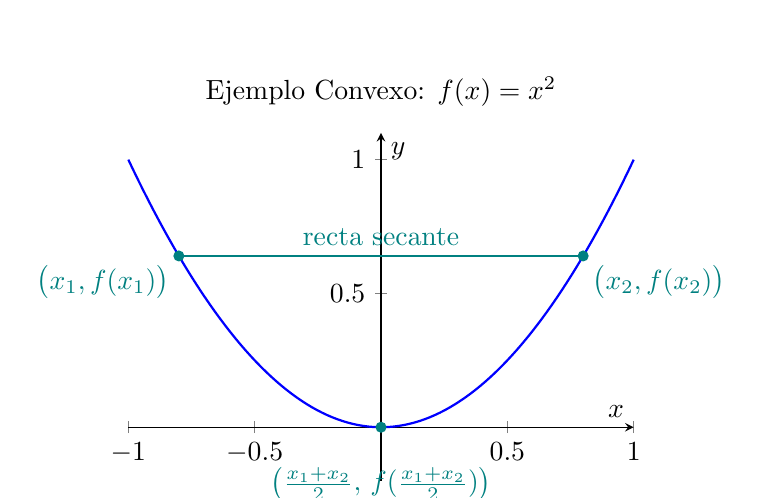
\begin{tikzpicture}
  \begin{axis}[
    width=8cm, height=6cm,
    axis lines=middle,
    xlabel=$x$, ylabel=$y$,
    title={Ejemplo Convexo: $f(x)=x^2$},
    xmin=-1, xmax=1, ymin=-0.2, ymax=1.1,
    domain=-1:1, samples=100,
    clip=false
  ]
    % Gráfica de f(x)=x^2
    \addplot[thick,blue] {x^2};

    % Puntos (x1, f(x1)) y (x2, f(x2))
    \coordinate (P1) at (axis cs:-0.8,0.64);
    \coordinate (P2) at (axis cs: 0.8,0.64);
    \fill[teal] (P1) circle (2pt) node[below left]  {$\bigl(x_1,f(x_1)\bigr)$};
    \fill[teal] (P2) circle (2pt) node[below right] {$\bigl(x_2,f(x_2)\bigr)$};

    % Recta secante
    \draw[teal, thick] (P1) -- (P2) node[midway, above] {recta secante};

    % Punto medio en x = (x1+x2)/2
    \coordinate (Pm) at (axis cs:0,0);
    \fill[teal] (Pm) circle (2pt) node[below=11pt] {
      $\bigl(\tfrac{x_1+x_2}{2},\,f(\tfrac{x_1+x_2}{2})\bigr)$
    };
  \end{axis}
\end{tikzpicture}
\end{center}

\begin{center}
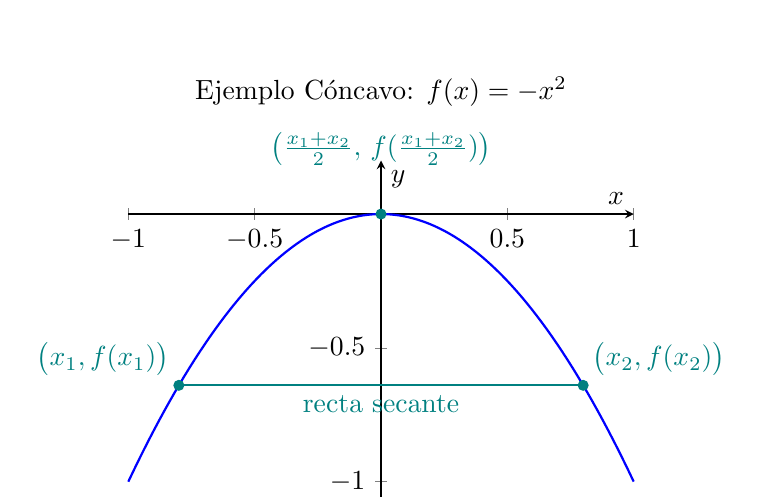
\begin{tikzpicture}
  \begin{axis}[
   title style={yshift=1em},
    width=8cm, height=6cm,
    axis lines=middle,
    xlabel=$x$, ylabel=$y$,
    title={Ejemplo Cóncavo: $f(x)=-x^2$},
    xmin=-1, xmax=1, ymin=-1.1, ymax=0.2,
    domain=-1:1, samples=100,
    clip=false
  ]
    % Gráfica de f(x) = -x^2
    \addplot[thick,blue] {-x^2};

    % Puntos (x1, f(x1)) y (x2, f(x2))
    \coordinate (Q1) at (axis cs:-0.8,-0.64);
    \coordinate (Q2) at (axis cs: 0.8,-0.64);
    \fill[teal] (Q1) circle (2pt) node[above left]  {$\bigl(x_1,f(x_1)\bigr)$};
    \fill[teal] (Q2) circle (2pt) node[above right] {$\bigl(x_2,f(x_2)\bigr)$};

    % Recta secante
    \draw[teal, thick] (Q1) -- (Q2) node[midway, below] {recta secante};

    % Punto medio en x = (x1+x2)/2
    \coordinate (Qm) at (axis cs:0,0);
    \fill[teal] (Qm) circle (2pt) node[above=14pt] {
      $\bigl(\tfrac{x_1+x_2}{2},\,f(\tfrac{x_1+x_2}{2})\bigr)$
    };
  \end{axis}
\end{tikzpicture}
\end{center}

\subsection*{Relacionando la concavidad y convexidad con conjuntos convexos}

\begin{itemize}
  \item \emph{Convexidad:} la región
    \[
      \bigl\{(x,y)\mid y \ge f(x)\bigr\}
    \]
    es un conjunto convexo. Esto significa que si tomas dos puntos
    \((x_1,y_1)\) y \((x_2,y_2)\) por encima del gráfico de \(f\),
    el segmento que los une permanece siempre por encima de la curva
  \item \emph{Concavidad:} la región
    \[
      \bigl\{(x,y)\mid y \le f(x)\bigr\}
    \]
    es un conjunto convexo. En este caso, cualquier segmento trazado
    entre dos puntos por debajo del gráfico de \(f\) queda enteramente
    dentro de esa región
\end{itemize}

\begin{center}
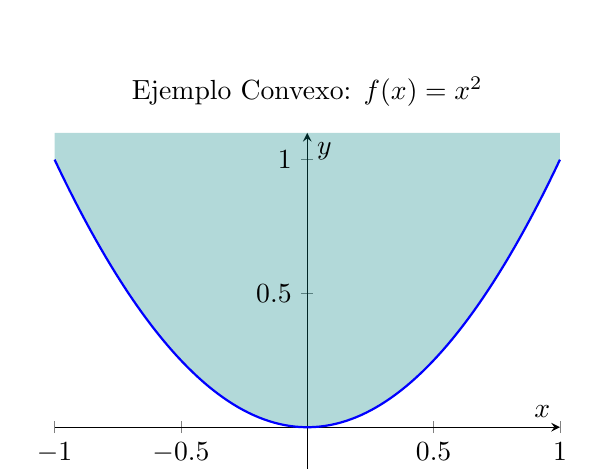
\begin{tikzpicture}
  \begin{axis}[
    width=8cm, height=6cm,
    axis lines=middle,
    xlabel=$x$, ylabel=$y$,
    title={Ejemplo Convexo: $f(x)=x^2$},
    xmin=-1, xmax=1, ymin=-0.2, ymax=1.1,
    domain=-1:1,
    samples=100,
    clip=false
  ]
    % 1. Define la curva f(x)=x^2 (sin dibujarla aún, solo para la ruta)
    \addplot[draw=none, name path=f_curve, domain=-1:1, samples=100] {x^2};

    % 2. Define la línea superior (y=ymax)
    \addplot[draw=none, name path=top_boundary,
             domain=\pgfkeysvalueof{/pgfplots/xmin}:\pgfkeysvalueof{/pgfplots/xmax},
             samples=2]
             {\pgfkeysvalueof{/pgfplots/ymax}};

    % 3. Rellena el área entre f_curve y top_boundary
    \addplot[teal, fill opacity=0.3] fill between[of=f_curve and top_boundary];

    % 4. Dibuja la curva f(x)=x^2 encima del relleno
    \addplot[thick, blue, domain=-1:1, samples=100] {x^2};

  \end{axis}
\end{tikzpicture}
\end{center}

\begin{center}
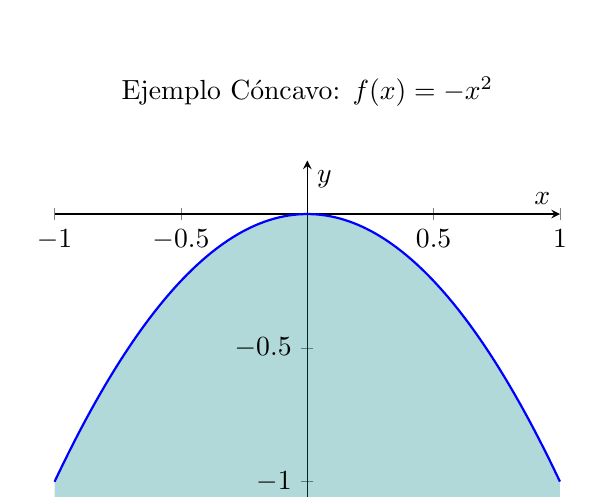
\begin{tikzpicture}
  \begin{axis}[
    title style={yshift=1em},
    width=8cm, height=6cm,
    axis lines=middle,
    xlabel=$x$, ylabel=$y$,
    title={Ejemplo Cóncavo: $f(x)=-x^2$},
    xmin=-1, xmax=1, ymin=-1.1, ymax=0.2,
    domain=-1:1,
    samples=100,
    clip=false
  ]
    % 1. Define la curva f(x)=-x^2
    \addplot[draw=none, name path=f_curve_concave, domain=-1:1, samples=100] {-x^2};

    % 2. Define la línea inferior (y=ymin)
    \addplot[draw=none, name path=bottom_boundary,
             domain=\pgfkeysvalueof{/pgfplots/xmin}:\pgfkeysvalueof{/pgfplots/xmax},
             samples=2]
             {\pgfkeysvalueof{/pgfplots/ymin}};

    % 3. Rellena el área entre f_curve_concave y bottom_boundary
    \addplot[teal, fill opacity=0.3] fill between[of=f_curve_concave and bottom_boundary];

    % 4. Dibuja la curva f(x)=-x^2 encima del relleno
    \addplot[thick, blue, domain=-1:1, samples=100] {-x^2};

  \end{axis}
\end{tikzpicture}
\end{center}


\section*{Concavidad y convexidad en $\R^2$}

\noindent\textbf{Definición:}
\begin{itemize}
  \item \(f\) es \emph{convexa} si para todo \((x_1,y_1)\), \((x_2,y_2)\) y todo \(t\in[0,1]\) se cumple
  \[
    \color{teal}
    f\bigl((1-t)(x_1,y_1)+t(x_2,y_2)\bigr)
    \;\le\;
    (1-t)\,f(x_1,y_1) + t\,f(x_2,y_2)
  \]
  \item \(f\) es \emph{cóncava} si \(-f\) es convexa, es decir la desigualdad se invierte
\end{itemize}

\noindent\textbf{Intuición geométrica:} La intuición se mantiene, el conjunto que está por debajo de la gráfica de una función cóncava es un conjunto convexo y el conjunto que está por arriba de una función convexa es un conjunto convexo

\section*{Regla en base a derivadas segundas}

\noindent\textbf{Recordatorio: criterio para funciones de una variable}\\
Sea \(g\colon I\subset\mathbb{R}\to\mathbb{R}\) de clase \(C^2\) en un intervalo \(I\). Entonces
\[
\begin{cases}
g''(t)\ge0\quad\forall\,t\in I
&\Longrightarrow\;g\text{ es convexa en }I\\[6pt]
g''(t)\le0\quad\forall\,t\in I
&\Longrightarrow\;g\text{ es cóncava en }I
\end{cases}
\]

\noindent\textbf{Sea \(f\colon\mathbb{R}^2\to\mathbb{R}\) de clase \(C^2\).}\\

Tomemos dos puntos \((x_1,y_1)\) y \((x_2,y_2)\) en \(\R^2\) y sea
\[
g(t) \;=\; f\bigl((1-t)x_1 + t\,x_2,\;(1-t)y_1 + t\,y_2\bigr)
\quad t\in[0,1]
\]

\noindent\textbf{Intuición sobre \(g\).}  
Para entender qué hace \(g\), primero observemos que  
\[
(x(t),y(t)) \;=\;\bigl((1-t)x_1 + t\,x_2,\;(1-t)y_1 + t\,y_2\bigr)
\]
es la parametrización del segmento rectilíneo que une los puntos \((x_1,y_1)\) y \((x_2,y_2)\) en el plano  
Por tanto,
\[
g(t) \;=\; f\bigl(x(t),y(t)\bigr)
\]
No es más que el valor de \(f\) al desplazarnos a lo largo de ese segmento  
\begin{itemize}
    \item Cuando \(t=0\) estamos en \((x_1,y_1)\)  
    \item Cuando \(t=1\) estamos en \((x_2,y_2)\)  
    \item Para \(t\in(0,1)\) recorremos los puntos intermedios  
\end{itemize}

Por la regla de la cadena aplicada a dos variables:
\[
\begin{aligned}
g'(t)
&= f_x\bigl(x(t),y(t)\bigr)\,\frac{d}{dt}\bigl((1-t)x_1 + t\,x_2\bigr)
 + f_y\bigl(x(t),y(t)\bigr)\,\frac{d}{dt}\bigl((1-t)y_1 + t\,y_2\bigr)\\[4pt]
&= f_x(x(t),y(t))\,(x_2 - x_1)
 + f_y(x(t),y(t))\,(y_2 - y_1)
\end{aligned}
\]

\[
\begin{aligned}
g''(t)
&= \frac{d}{dt}\bigl[f_x(x(t),y(t))\bigr]\,(x_2 - x_1)
 + \frac{d}{dt}\bigl[f_y(x(t),y(t))\bigr]\,(y_2 - y_1)\\[6pt]
&= \bigl[f_{xx}(x(t),y(t))\,x'(t)
        + f_{xy}(x(t),y(t))\,y'(t)\bigr]\,(x_2 - x_1)\\
&\quad
 + \bigl[f_{yx}(x(t),y(t))\,x'(t)
        + f_{yy}(x(t),y(t))\,y'(t)\bigr]\,(y_2 - y_1)
\end{aligned}
\]

Sabiendo que \(x'(t)=x_2-x_1\) y \(y'(t)=y_2-y_1\):
\[
\begin{aligned}
g''(t)
&= f_{xx}(x(t),y(t))\,(x_2 - x_1)\,(x_2 - x_1)
+ f_{xy}(x(t),y(t))\,(y_2 - y_1)\,(x_2 - x_1)\\
&\quad
+ f_{yx}(x(t),y(t))\,(x_2 - x_1)\,(y_2 - y_1)
+ f_{yy}(x(t),y(t))\,(y_2 - y_1)\,(y_2 - y_1)
\end{aligned}
\]

Usando \(f_{xy}=f_{yx}\), se agrupan los términos mixtos:
\[
g''(t)
= f_{xx}(x(t),y(t))\,(x_2 - x_1)^2
+ 2\,f_{xy}(x(t),y(t))\,(x_2 - x_1)(y_2 - y_1)
+ f_{yy}(x(t),y(t))\,(y_2 - y_1)^2
\]

Redefiniendo para mayor claridad:
\[
\begin{aligned}
w &= x_2 - x_1
\qquad
z = y_2 - y_1\\[6pt]
g''(t)
&= f_{xx}\bigl(x(t),y(t)\bigr)\,w^2
 + 2\,f_{xy}\bigl(x(t),y(t)\bigr)\,w\,z
 + f_{yy}\bigl(x(t),y(t)\bigr)\,z^2\\[6pt]
&= \color{teal}
\begin{pmatrix}w & z\end{pmatrix}
\begin{pmatrix}
f_{xx}\bigl(x(t),y(t)\bigr) & f_{xy}\bigl(x(t),y(t)\bigr)\\[4pt]
f_{xy}\bigl(x(t),y(t)\bigr) & f_{yy}\bigl(x(t),y(t)\bigr)
\end{pmatrix}
\begin{pmatrix}w\\[4pt]z\end{pmatrix}
\end{aligned}
\]

\noindent Ahora, si la matriz Hessiana
\(\;H_f(x,y)=\bigl[f_{ij}(x,y)\bigr]\)
es semidefinida positiva en todo punto, entonces para cada \(t\in[0,1]\)
\[
g''(t)\;\ge\;0
\]
Lo cual implica que \(g\) es convexa  

Definamos la \emph{recta secante} entre \((0,g(0))\) y \((1,g(1))\):
\[
L(t) \;=\; g(0)\;+\;t\bigl(g(1)-g(0)\bigr)
\;=\;(1-t)\,g(0) \;+\; t\,g(1)
\]

Si la Hessiana \(H_f(x,y)\) es semidefinida positiva, entonces \(g''(t)\ge0\) en \([0,1]\), lo que por teoría de funciones de una variable implica
\[
g(t)\;\le\;L(t)\;=\;(1-t)\,g(0) + t\,g(1)
\]

Finalmente, usando \(g(0)=f(x_1,y_1)\) y \(g(1)=f(x_2,y_2)\), concluimos
\[
\color{teal}
f\bigl((1-t)(x_1,y_1)+t\,(x_2,y_2)\bigr)
\;=\;g(t)
\;\le\;
(1-t)\,f(x_1,y_1) \;+\; t\,f(x_2,y_2)
\]
\textbf{\color{teal}que es precisamente la condición de convexidad de \(f\) en \(\mathbb{R}^2\)}

De forma análoga, si \(H_f\) es semidefinida \emph{negativa}, entonces
\[
\color{teal}
g''(t)\le0
\quad\Longrightarrow\quad
g(t)\ge(1-t)\,g(0)+t\,g(1)
\]
\textbf{\color{teal}y por tanto \(f\) es \emph{cóncava}}
%%%%%%%%%%%%%%%%%%%%%%%%%%

\subsection*{Extensión a $\R^n$}
El mismo argumento—considerar la función unidimensional  
\(\;g(t)=f\bigl((1-t)x + t\,y\bigr)\)—se aplica en \(\R^n\). Si la matriz de derivadas segundas (matriz hessiana) es semidefinida positiva para todo \(x\), entonces en cada dirección \(y-x\)  
la derivada segunda \(g''(t)\ge0\), lo que implica la convexidad de \(g\)  
y, por tanto, la convexidad de \(f\). Análogamente, semidefinida negativa  
da concavidad de \(f\) en \(\R^n\)

\noindent Además, si la Hessiana \(H_f(x)\) es \emph{definida positiva} en todo punto, entonces \(f\) es \emph{estrictamente convexa}; y si \(H_f(x)\) es \emph{definida negativa} en todo punto, entonces \(f\) es \emph{estrictamente cóncava}

\noindent\textbf{En resumen}
\[
\renewcommand{\arraystretch}{1.25}
\begin{array}{|c|l|c|}
\hline
\textbf{\color{teal}Hessiana } H_f(x)
  & \textbf{\color{teal}Condición (}\forall x\in D\ \text{convexo},\ \forall h\in\mathbb{R}^n\textbf{)}
  & \textbf{\color{teal}Función \(f\)} \\ \hline
\text{Semidefinida positiva}
  & h^{T} H_f(x)\, h \;\ge\; 0
  & \text{Convexa} \\ \hline
\text{Definida positiva}
  & h^{T} H_f(x)\, h \;>\; 0 \quad \text{para todo } h\neq 0
  & \text{Estr. convexa} \\ \hline
\text{Semidefinida negativa}
  & h^{T} H_f(x)\, h \;\le\; 0
  & \text{Cóncava} \\ \hline
\text{Definida negativa}
  & h^{T} H_f(x)\, h \;<\; 0 \quad \text{para todo } h\neq 0
  & \text{Estr. cóncava} \\ \hline
\end{array}
\]
{\small (Aquí \(D\) denota el dominio de \(f\).)}


\subsection*{Ejemplo}

Consideremos la función
\[
f(x,y) \;=\; x^2 \;+\; 2\,x\,y \;+\; 3\,y^2
\qquad (x,y)\in\R^2
\]

\medskip

\noindent\textbf{Cálculo del Hessiano}\\
Las segundas derivadas parciales son
\[
f_{xx} = 2,\quad
f_{xy} = 2,\quad
f_{yy} = 6
\]
Por tanto la matriz Hessiana es
\[
H_f(x,y)
=\begin{pmatrix}
2 & 2\\[4pt]
2 & 6
\end{pmatrix}
\]

\medskip

\noindent\textbf{Comprobación de definitud (criterio de Sylvester).}\\
Calculamos los menores principales iniciales:
\[
\Delta_1 = f_{xx} = 2 > 0
\qquad
\Delta_2 = \det H_f = (2)(6) - (2)^2 = 12 - 4 = 8 > 0
\]
Como \(\Delta_1>0\) y \(\Delta_2>0\), \(H_f\) es \emph{definida positiva} en todo \(\R^2\)

\medskip

\noindent\textbf{Conclusión:}\\
{\color{teal}Al ser su Hessiana definida positiva para todo \((x,y)\), la función \(f\) es \emph{estrictamente convexa} en \(\R^2\)}

\subsection*{Otro ejemplo}

Consideremos 
\[
f(x,y) = -\,x^2
\qquad (x,y)\in\R^2
\]

\medskip
\noindent\textbf{Cálculo del Hessiano}\\
\[
f_{xx} = -2,\quad
f_{xy} = 0,\quad
f_{yy} = 0
\]
Por tanto la matriz Hessiana es
\[
H_f(x,y) = 
\begin{pmatrix}
-2 & 0\\[4pt]
0  & 0
\end{pmatrix}
\]

\medskip
\noindent\textbf{Comprobación de semidefinición.}\\
Los menores principales iniciales son
\[
\Delta_1 = f_{xx} = -2 < 0
\qquad
\Delta_2 = \det H_f = (-2)\cdot0 - 0^2 = 0
\]
Como \(\Delta_1<0\) y \(\Delta_2=0\), debemos analizar un menor principal más: \(\Delta_1^{2,2}=0\leq0\), entonces \(H_f\) es \emph{semidefinida negativa} (pero no definida negativa)

\medskip
\noindent\textbf{Conclusión.}\\
\textbf{\color{teal}Al ser su Hessiana semidefinida negativa en todo \(\R^2\), \(f\) es \emph{cóncava}.  
Además, \(f\) no es convexa, ni estrictamente cóncava, ni estrictamente convexa}

\section*{Cuasiconcavidad y cuasiconvexidad}

\noindent Primero, observemos que:
\begin{itemize}
  \item Toda función \emph{cóncava} es \emph{cuasicóncava}
  \item Toda función \emph{convexa} es \emph{cuasiconvexa}
\end{itemize}





%%%%%%%%%%%%%%%%%%%%%%%







\noindent\textbf{Caracterización de cuasiconvexidad y cuasiconcavidad}
\begin{itemize}
  \item \color{teal}\(f\) es \emph{cuasiconvexa} si y solo si todos sus \emph{subniveles} \(L_\alpha(f)\) son conjuntos convexos
  \item \color{teal}\(f\) es \emph{cuasicóncava} si y solo si todos sus \emph{superniveles} \(U^\alpha(f)\) son conjuntos convexos
\end{itemize}

\noindent\textbf{Interpretación en curvas de nivel}\\
Recordemos que las \emph{curvas de nivel} de \(f\) para un valor \(\alpha\) son los conjuntos
\[
\{\,x\in\R^n : f(x)=\alpha\}
\]
Los conjuntos de nivel (subniveles y superniveles) son las regiones delimitadas por esas curvas:
\[
\begin{aligned}
L_\alpha(f) &= \{\,x\in\R^n : f(x)\le \alpha\}\\[4pt]
U^\alpha(f) &= \{\,x\in\R^n : f(x)\ge \alpha\}
\end{aligned}
\]

\section*{Criterio de hessiano orlado para cuasiconvexidad y cuasiconcavidad}
Las siguientes condiciones son válidas cuando evaluamos las funciones en números positivos (es decir en el ortante no negativo):\\
Sea \(f\colon U\subseteq\mathbb{R}^n\to\mathbb{R}\) de clase \(C^2\) en un dominio convexo \(U\), y supongamos \(\nabla f(x)\neq0\) para todo \(x\in U\). Definimos la \emph{matriz hessiano orlado} en \(x\) como
\[
B(x)
=\begin{pmatrix}
0 & \nabla f(x)^T \\[4pt]
\nabla f(x) & H_f(x)
\end{pmatrix}
\]
donde \(H_f(x)\) es la Hessiana usual de \(f\)

\noindent Entonces se tiene la caracterización siguiente:

Condiciones necesarias:
\begin{itemize}
  \item {\color{teal}\(f\) es cuasiconvexa en \(U\) solo si los menores principales de orden inicial (sin contar el 0) son todos menores o iguales a 0}
  \item {\color{teal}\(f\) es cuasicóncava en \(U\) solo si los menores principales de orden inicial (sin contar el 0) alternan de signo (o son iguales a 0) empezando por el negativo}
\end{itemize}

Condiciones suficientes y que además aseguran cuasiconcavidad y cuasiconvexidad estricta:
\begin{itemize}
  \item {\color{teal}\(f\) es cuasiconvexa en \(U\) si los menores principales de orden inicial (sin contar el 0) son todos menores a 0}
  \item {\color{teal}\(f\) es cuasicóncava en \(U\) si los menores principales de orden inicial (sin contar el 0) alternan de signo empezando por el negativo}
\end{itemize}

Para que \(z = f(x_1,\dots,x_n)\) sea cuasicóncava en el \(n\)-ortante no negativo, es necesario que
\[
\color{teal}
|B_1| \le 0,\quad
|B_2| \ge 0,\quad
\dots,\quad
|B_n|
\begin{cases}
\le 0 & n\text{ impar}\\
\ge 0 & n\text{ par}
\end{cases}
\]

Una condición suficiente para que \(f\) sea \emph{cuasicóncava} en el \(n\)-ortante no negativo es que
\[
\color{teal}
|B_1| < 0,\quad
|B_2| > 0,\quad
\dots,\quad
|B_n|
\begin{cases}
< 0 & n\text{ impar}\\[4pt]
> 0 & n\text{ par}
\end{cases}
\]

\subsection*{Ejemplo}

Sea 
\[
f\colon A\to\R,
\qquad
A=\{(x,y)\in\R^2:x>0,\;y>0\},
\quad
f(x,y)=x\,y
\]

\medskip

\noindent\textbf{Derivadas parciales y Hessiano}\\
\[
f_x = y,\quad f_y = x,
\qquad
H_f(x,y)
= \begin{pmatrix}
0 & 1\\[4pt]
1 & 0
\end{pmatrix}
\]

\medskip

\noindent\textbf{Hessiano orlado}\\
Definimos las siguientes matrices:
\[
B_1 = 
\begin{pmatrix}
0 & y\\[4pt]
y & 0
\end{pmatrix}
\qquad
B_2 =
\begin{pmatrix}
0 & y & x\\[4pt]
y & 0 & 1\\[4pt]
x & 1 & 0
\end{pmatrix}
\]

\medskip

\noindent\textbf{Cálculo de determinantes}\\
\[
\det B_1 = -\,y^2<0
\qquad
\det B_2 = 2\,x\,y \;>\;0
\]

\medskip

\noindent\textbf{Conclusión}\\
Para cuasiconcavidad en el dominio convexo \(A\) se exige
\[
D_1 <0,\quad D_2\ge0
\]
Como \(x,y>0\) garantizan \(D_1<0\) y \(D_2>0\), concluimos que
\[
\color{teal}
f(x,y)=x\,y\text{ es cuasicóncava en }A
\]






\section*{Relación y diferencias entre cuasiconcavidad y concavidad (o cuasiconvexidad y convexidad)}

\begin{itemize}
  \item \textbf{Relación entre ambas:}
    \begin{itemize}
      \item Toda función \emph{cóncava} es \emph{cuasicóncava}
      \item La recíproca no es cierta: hay funciones cuasicóncavas que no son cóncavas
      \item Toda función \emph{convexa} es \emph{cuasiconvexa}
      \item La recíproca no es cierta: hay funciones cuasiconvexas que no son convexas
    \end{itemize}

  \item \textbf{Operaciones y composición:}
    \begin{itemize}
      \item Suma y combinación lineal (con coeficientes no negativos) de cóncavas/convexas produce una función cóncava/convexa
      \item La suma de funciones cuasicóncavas/cuasiconvexas no siempre es cuasicóncava/cuasiconvexa
      \item La cuasiconcavidad/cuasiconvexidad se conserva bajo composición con funciones estrictamente crecientes
      \item Además, sea
      \[
        h(x) = (g\circ f)(x)
      \]
      con
      \[
        f\colon M\subseteq\mathbb{R}^n\to\mathbb{R},
        \quad
        g\colon I\subseteq\mathbb{R}\to\mathbb{R}
      \]
      donde \(M\) es convexo e \(I\) es un intervalo. Entonces:
      \begin{enumerate}
        \item Si \(f\) es convexa y \(g\) es creciente y convexa, entonces \(h\) es convexa
        \item Si \(f\) es cóncava y \(g\) es creciente y cóncava, entonces \(h\) es cóncava
      \end{enumerate}
    \end{itemize}
\end{itemize}

\subsection*{Ejemplo}

Anteriormente probamos que \(f(x,y)=xy\) es cuasicóncava. Veamos una transformación de dicha función: sea
\[
g(x,y)=\ln(xy)=\ln x+\ln y
\]
\[
g_x=\frac1x,\quad g_y=\frac1y,
\qquad
g_{xx}=-\frac1{x^2},\;g_{xy}=0,\;g_{yy}=-\frac1{y^2}
\]

\[
B_1(x,y)
=\begin{pmatrix}
0 & g_x\\[4pt]
g_x & g_{xx}
\end{pmatrix}
=
\begin{pmatrix}
0 & \tfrac1x\\[4pt]
\tfrac1x & -\tfrac1{x^2}
\end{pmatrix}
\]

\[
D_1(x,y)=\det B_1=-\frac1{x^2}<0
\]

\[
B_2(x,y)
=\begin{pmatrix}
0      & g_x       & g_y\\[4pt]
g_x    & g_{xx}    & g_{xy}\\[4pt]
g_y    & g_{xy}    & g_{yy}
\end{pmatrix}
=
\begin{pmatrix}
0      & \tfrac1x       & \tfrac1y\\[4pt]
\tfrac1x & -\tfrac1{x^2} & 0\\[4pt]
\tfrac1y & 0             & -\tfrac1{y^2}
\end{pmatrix}
\]

\[
D_2(x,y)=\det B_2=\frac{2}{x^2\,y^2}>0
\]

\noindent\textbf{Conclusión}\\
\[
D_1<0,\quad D_2>0
\]
\textbf{\color{teal}Por tanto \(g(x,y)=\ln(xy)\) es \emph{cuasicóncava} en \(A\)}








\newpage
\section{Optimización sin restricciones}


\section*{Optimización sin restricciones: cálculo univariable}

Sea \(f\colon I\subseteq\mathbb{R}\to\mathbb{R}\) una función de clase \(C^2\).  
Para encontrar extremos locales de \(f\) aplicamos el siguiente procedimiento:

\begin{enumerate}
  \item \textbf{Condición de primer orden:}  
    Calcular la derivada primera y resolver
    \[
      f'(x^*) = 0
    \]
    Los puntos \(x^*\) que satisfacen esta ecuación son los \emph{puntos críticos}.

  \item \textbf{Condición de segundo orden:}  
    Evaluar la derivada segunda en cada \(x^*\):
    \[\color{teal}
      f''(x^*) \begin{cases}
        >0 & \Rightarrow\;x^*\text{ es un mínimo local}\\[4pt]
        <0 & \Rightarrow\;x^*\text{ es un máximo local}\\[4pt]
        =0 & \Rightarrow\;\text{criterio inconcluso (punto de inflexión posible)}
      \end{cases}
    \]
\end{enumerate}

\medskip

\noindent\emph{Ejemplo rápido:}  
Para \(f(x)=x^3-3x\):
\[
f'(x)=3x^2-3,\;f'(x)=0\Rightarrow x=\pm1;
\quad
f''(x)=6x.
\]
\[
f''(1)=6>0\;\Rightarrow\;x=1\text{ mínimo local},\qquad
\color{teal} f''(-1)=-6<0\;\Rightarrow\;x=-1\text{ máximo local}.
\]

\section*{Pasando a \(n\) variables}

% Definición previa de x como vector
Denotemos 
\[
x = (x_{1}, x_{2}, \dots, x_{n}) \in \mathbb{R}^n
\]
y sea 
\[
x^* = (x^*_{1}, x^*_{2}, \dots, x^*_{n})
\]
un punto crítico en \(\mathbb{R}^n\).

\[
F\colon A\subseteq\mathbb{R}^n\;\to\;\mathbb{R}
\]
la \emph{condición de primer orden} generaliza a  
\[
\nabla F(x^*) = \mathbf{0}
\]
es decir, todas las derivadas parciales en \(x^*\) deben anularse.  

La \emph{condición de segundo orden} se extrae de la matriz Hessiana  
\(H=\nabla^2 F(x)\), que reúne todas las derivadas segundas de \(F\).  
De la misma manera que \(f''(x^*)\) en una variable nos indica concavidad o convexidad,  
la semidefinición positiva o negativa de  $H$ nos permitirá determinar si \(F\) tiene un mínimo o máximo local en \(x^*\).


\subsection*{Condiciones suficientes y criterio de la matriz Hessiana}

Sea 
\[
F\colon U\subseteq\mathbb{R}^n\;\longrightarrow\;\mathbb{R}
\]
de clase \(C^2\) y sea \(x^*\in U\) un punto crítico, es decir,
\[
\nabla F(x^*) = \mathbf{0}.
\]

\begin{itemize}

  \item \textbf{Óptimo local (criterio de la Hessiana).}
    \begin{itemize} \color{teal}
      \item \color{teal}Si \(H(x^*)\) es \emph{definida negativa}, entonces \(x^*\) es \emph{máximo local}.
      \item Si \(H(x^*)\) es \emph{definida positiva}, entonces \(x^*\) es \emph{mínimo local}.
      \item Si \(H(x^*)\) es \emph{indefinida}, entonces \(x^*\) no es ni mínimo ni máximo local (punto silla).
    \end{itemize}
      \item \textbf{Óptimo global (funciones convexas o cóncavas).}
    \begin{itemize}
      \item \color{teal} Si \(F\) es convexa en \(U\) y \(\nabla F(x^*)=0\), entonces \(x^*\) es \emph{mínimo global}.
      \item Si \(F\) es cóncava en \(U\) y \(\nabla F(x^*)=0\), entonces \(x^*\) es \emph{máximo global}.
    \end{itemize}
\end{itemize}

\subsection*{Criterio de los menores principales para óptimo local.}

Sea 
\[
F\colon U\subseteq\mathbb{R}^n\;\longrightarrow\;\mathbb{R}
\]
de clase \(C^2\) y supongamos que \(x^*\in U\) es un punto crítico:
\[
\nabla F(x^*) = \mathbf{0}
\]
Denotemos $\Delta_k$ por el menor principal inicial de orden \(k\) de la matriz Hessiana evaluada en el punto crítico.

\medskip

\noindent\textbf{Condición para máximo local.}  
Si los menores principales alternan de signo comenzando negativo:
\[\color{teal}
\Delta_1 < 0,\quad \Delta_2 > 0,\quad \Delta_3 < 0,\;\dots,\;(-1)^n\,\Delta_n > 0
\]
entonces \(x^*\) es un \emph{máximo local } de \(F\).

\medskip

\noindent\textbf{Condición para mínimo local .}  
Si todos los menores principales son positivos:
\[\color{teal}
\Delta_1 > 0,\quad \Delta_2 > 0,\quad \Delta_3 > 0,\;\dots,\;\Delta_n > 0
\]
entonces \(x^*\) es un \emph{mínimo local } de \(F\).



\subsection*{Criterio de los menores principales para óptimo global}


\noindent\textbf{Mínimo global.}  
Para que \(F\) tenga un \emph{mínimo global} en \(U\), es suficiente que la matriz Hessiana \(H\) sea semidefinida positiva en \emph{todos} los puntos \(x\in U\). \textbf{\color{teal}En términos de menores principales, esto equivale a que para \emph{cualquier} submatriz principal (es decir, para cualquier selección de filas y columnas con los mismos índices) el determinante sea mayor o igual a cero}. Cuando esto se cumple, \(F\) es convexa y cualquier punto crítico es automáticamente un mínimo global.

\medskip

\noindent\textbf{Máximo global.}  
Análogamente, \(F\) tiene un \emph{máximo global} en \(U\) si la Hessiana \(H\) es semidefinida negativa en todo \(U\). \textbf{\color{teal}En lenguaje de menores principales, esto significa que para cada submatriz principal de orden \(k\), el determinante de dicha submatriz multiplicado por \((-1)^k\) es mayor o igual a cero.} Bajo esta condición, \(F\) es cóncava y cada punto crítico será un máximo global.



\subsection*{Diferencia entre óptimos locales y globales}
La principal diferencia entre óptimos que son locales y óptimos globales es que al momento de realizar el cálculo de segundas derivadas (con la matriz hessiana), para asegurar un óptimo local tenemos que evaluar el hessiano en un punto particular, de tal forma de mostrar la función tiene un comportamiento similar al de una función estrictamente convexa/cóncava en la vecindad inmediata de $x^*$. Por otro lado, para poder confirmar que un óptimo es global es necesario analizar la forma de la función, analizando el hessiano sin evaluar en ningún punto particular y ver si la función es convexa o cóncava.



\section*{Ejemplo: \(F(x,y)=x^3 - y^3 + 9xy\)}

\subsection*{1. Derivadas parciales y puntos críticos}

Definimos
\[
F(x,y)=x^3 - y^3 + 9\,x\,y
\]
Calculamos las derivadas parciales:
\[
F_x = \frac{\partial F}{\partial x}
= 3x^2 + 9y
\qquad
F_y = \frac{\partial F}{\partial y}
= -3y^2 + 9x
\]
Para hallar los puntos críticos resolvemos
\[
\begin{cases}
3x^2 + 9y = 0\\[6pt]
-3y^2 + 9x = 0
\end{cases}
\]
De la primera ecuación:
\[
y = -\frac{x^2}{3}
\]
Sustituyendo en la segunda:
\[
-3\Bigl(-\tfrac{x^2}{3}\Bigr)^2 + 9x = 0
\;\Longrightarrow\;
-3\;\frac{x^4}{9} + 9x = 0
\;\Longrightarrow\;
-\tfrac{x^4}{3} + 9x = 0
\;\Longrightarrow\;
-x^4 + 27x = 0
\;\Longrightarrow\;
x\,( -x^3 + 27 ) = 0
\]
De aquí obtenemos
\[
x=0
\quad\Longrightarrow\quad y=0,
\qquad
-x^3 + 27 = 0
\;\Longrightarrow\;
x^3 = 27
\;\Longrightarrow\;
x = 3
\;\Longrightarrow\;
y = -\frac{3^2}{3} = -3
\]
Por tanto, los puntos críticos son
\[\color{teal}
(0,0)
\quad\text{y}\quad
(3,-3)
\]

\subsection*{2. Hessiano y clasificación de extremos}

El Hessiano es
\[
\nabla^2 F(x,y)
=
\begin{pmatrix}
F_{xx} & F_{xy}\\[4pt]
F_{yx} & F_{yy}
\end{pmatrix}
=
\begin{pmatrix}
6x & 9\\[4pt]
9  & -6y
\end{pmatrix}
\]

\begin{enumerate}
  \item \textbf{En \((0,0)\):}
  \[
  \nabla^2 F(0,0)
  = \begin{pmatrix}0 & 9\\[4pt]9 & 0\end{pmatrix},
  \quad \Delta_1 = 0,\quad
  \Delta_2  = -81 < 0
  \]
  Como \(\Delta_2<0\), es un punto silla (saddle point).

  \item \textbf{En \((3,-3)\):}
  \[
  \nabla^2 F(3,-3)
  = \begin{pmatrix}18 & 9\\[4pt]9 & 18\end{pmatrix},
  \quad \Delta_1 = 18 > 0,\quad
  \Delta_2 = 18\cdot18 - 9\cdot9 = 243 > 0
  \]
  Aquí la Hessiana es definida positiva, por lo que \((3,-3)\) es un mínimo local.
\end{enumerate}

\medskip

\noindent\textbf{Conclusión:}
\begin{itemize}
  \item \color{teal} \((0,0)\) es un punto silla.
  \item \color{teal} \((3,-3)\) es un mínimo local de \(F\).
  \item \color{teal} No hay máximos locales.
\end{itemize}

\subsection*{3. Concavidad/convexidad global de \(F\)}

Para determinar si los extremos locales son también globales necesitamos ver si \(F\) es convexa o cóncava en todo \(\R^2\). Calculamos de nuevo el Hessiano general:

\[
\nabla^2 F(x,y)
=
\begin{pmatrix}
6x & 9\\[4pt]
9  & -6y
\end{pmatrix}
\]

Los menores principales siguen un patrón ya que por ejemplo $6x$, puede ser negativo o positivo. Lo mismo con $-6y$ y $|H|$. No podemos afirmar que tenemos un óptimo global.


\section*{Ejemplo: \(f(x,y)=x^2+y^2\)}

\subsection*{1. Derivadas parciales y punto crítico}

Sea 
\[
f(x,y)=x^2+y^2,\qquad (x,y)\in\R^2
\]
Calculamos las derivadas parciales:
\[
f_x=2x,\quad f_y=2y
\]
El único punto crítico se obtiene resolviendo
\[ \color{teal}
2x=0,\quad 2y=0
\;\Longrightarrow\;
(x,y)=(0,0)
\]

\subsection*{2. Hessiano y clasificación de extremos locales}

El Hessiano es constante:
\[
\nabla^2 f(x,y)
=
\begin{pmatrix}
2 & 0\\[4pt]
0 & 2
\end{pmatrix}
\]
Sus menores principales son
\[
\Delta_1^{1,1}=2>0,\qquad \Delta_1^{2,2}=2>0,\qquad
\Delta_2=\det\nabla^2f=4>0
\]
\textbf{\color{teal}de modo que la matriz es \emph{definida positiva} en todo \(\R^2\). Por el criterio de segundo orden, \((0,0)\) es un \emph{mínimo local}.
}
\subsection*{3. Convexidad global y mínimo global}

\textbf{\color{teal}Ya que \(\nabla^2f(x,y) \geq0\) en todo \(\R^2\), \(f\) es \emph{convexa} en \(\R^2\). En toda función convexa cualquier mínimo local es también \emph{mínimo global}. }

\section*{Óptimo local y global únicos}

\textbf{Teorema:} Sea \( f : D \to \mathbb{R} \) con \( D \subseteq \mathbb{R}^n \), abierto y convexo, \( f \in C^1(D) \) y sea \( \mathbf{x}_0 \in D \) un punto crítico de \( f \).

Se verifica:
\begin{enumerate}
    \item Si \( f \) es convexa en \( D \) entonces \( f \) presenta en \( \mathbf{x}_0 \) un mínimo global.
    \item Si \( f \) es estrictamente convexa en \( D \) entonces \( f \) presenta en \( \mathbf{x}_0 \) un mínimo global único.
    \item Si \( f \) es cóncava en \( D \) entonces \( f \) presenta en \( \mathbf{x}_0 \) un máximo global.
    \item Si \( f \) es estrictamente cóncava en \( D \) entonces \( f \) presenta en \( \mathbf{x}_0 \) un máximo global único.
\end{enumerate}



\section*{Preservación de máximos y mínimos locales en dos variables}


Sea $D \subseteq \mathbb{R}$ un conjunto abierto. Sea $\varphi: D \to \mathbb{R}$ una función de clase $C^2$ tal que $\varphi'(t)>0$ para todo $t \in D$. Sea $f:\mathbb{R}^2 \to \mathbb{R}$ una función de clase $C^2$ tal que su imagen está contenida en $D$ (es decir, $f(x,y) \in D$ para todo $(x,y)$ en el dominio de $f$ o en la región de interés).
Entonces:

\begin{enumerate}
  \item \((x_0,y_0)\) es punto crítico de \(f\) entonces \((x_0,y_0)\) es punto crítico de \(\varphi\circ f\).
  \item Si la matriz Hessiana \(D^2f(x_0,y_0)\) es definida negativa (máximo local) o definida positiva (mínimo local), la Hessiana de \(\varphi\circ f\) en \((x_0,y_0)\) mantiene la misma definitud.
\end{enumerate}

\medskip


\noindent\textbf{Ejemplos de \(\varphi\)}
\begin{itemize}
  \item \(\varphi(t)=a\,t + b\), con \(a>0\).
  \item \(\varphi(t)=\mathrm{e}^t\).
  \item \(\varphi(t)=\log(t + c)\), con \(c>0\) (dominio \(t>-c\)).
  \item \(\varphi(t)=t^3\) (con $t\neq0$ ).
  \item \(\varphi(t)=\sqrt{t}\) (en \(t>0\)).
\end{itemize}

\newpage

\section{Aplicaciones económicas de optimización}

\section*{Teorema de la envolvente (optimización sin restricciones)}

Consideremos el problema de maximización sin restricciones
\[
\max_{x,y}\;U \;=\;f(x,y,\phi)
\]
donde \(x,y\) son variables endógenas y \(\phi\) es un parámetro exógeno.  

\subsection*{Condiciones de óptimo}


Las condiciones necesarias de primer orden en el óptimo \((x^*(\phi),y^*(\phi))\) son
\begin{equation}\label{FOC}
\frac{\partial f}{\partial x}\bigl(x^*(\phi),\,y^*(\phi),\,\phi\bigr)=0,
\qquad
\frac{\partial f}{\partial y}\bigl(x^*(\phi),\,y^*(\phi),\,\phi\bigr)=0.
\end{equation}
Bajo condiciones de segundo orden adecuadas, estas ecuaciones definen implícitamente \(x^*(\phi)\) y \(y^*(\phi)\).

\[
x^*=x^*(\phi)
\qquad
y^*=y^*(\phi)
\]

\subsection*{Función de valor indirecta}

Sustituyendo en la función objetivo obtenemos la función de valor máximo (función objetivo indirecta)
\[
V(\phi) \;=\; f\bigl(x^*(\phi),\,y^*(\phi),\,\phi\bigr)
\]

Esta es una función que depende en última instancia de $\phi$, a diferencia de la función objetivo que depende de $x$ y de $y$.

\subsection*{Derivada de la función de valor}

Al diferenciar \(V\) con respecto a \(\phi\) usando la regla de la cadena:
\[
\frac{dV}{d\phi}
= f_x\,\frac{\partial x^*}{\partial\phi}
+ f_y\,\frac{\partial y^*}{\partial\phi}
+ f_\phi
\]
donde todos los términos \(f_x,f_y,f_\phi\) se evalúan en \(\bigl(x^*(\phi),y^*(\phi),\phi\bigr)\).  

Pero por las condiciones de primer orden \eqref{FOC} se tiene \(f_x=f_y=0\) en el óptimo, y por tanto
\[
\color{teal}
\frac{dV}{d\phi} \;=\; f_\phi\bigl(x^*(\phi),\,y^*(\phi),\,\phi\bigr)
\]
{\color{teal}Este es el \textbf{teorema de la envolvente}: la derivada de la función de valor máximo con respecto al parámetro \(\phi\) equivale al efecto directo de \(\phi\) sobre la función objetivo, ignorando los efectos indirectos vía \(x^*(\phi)\) y \(y^*(\phi)\).}

\subsection*{Interpretación}

\begin{itemize}
  \item La función de valor \(V(\phi)\) “envuelve” la familia de funciones \(f(x,y,\phi)\) optimizadas en \((x^*(\phi),y^*(\phi))\) al variar \(\phi\).
  \item El resultado muestra que, en el óptimo, no hace falta calcular \(\partial x^*/\partial\phi\) ni \(\partial y^*/\partial\phi\) para conocer \(\tfrac{dV}{d\phi}\): basta con el efecto directo \(f_\phi\).
\end{itemize}
%%%%%%%%%%%

\section*{Intuición: ¿Por qué ``teorema de la envolvente''?}

El nombre proviene de la idea geométrica de que la función de valor indirecta
\[
V(\phi)=\max_{x,y}f(x,y,\phi)
\]
es la \emph{envolvente} de la familia de gráficas
\(\{\,z=f(x,y,\phi):(x,y)\in\R^2\}\) al variar el parámetro \(\phi\). A continuación presentamos varias perspectivas:

\subsection*{Envolvente de familias de curvas/superficies}

Para cada \(\phi\) se tiene un punto en el plano \((\phi,z)\):
\[
z = f\bigl(x^*(\phi),y^*(\phi),\phi\bigr)
\]
Estos puntos conforman una curva al variar $\phi$. La curva límite que toca tangencialmente a cada una de estas es la \emph{envolvente}  
Gráficamente, \(V(\phi)\) “abraza” o “envuelve” el punto más alto de cada miembro de la familia


\subsection*{Ejemplo de envolvente con \(f(x;t)=t\,x^2 + x + 10\)}

Consideremos la familia de funciones
\[
f(x; t)=t\,x^2 + x + 10
\qquad x\in\R,\;t<0
\]
donde \(x\) es la variable de decisión y \(t\) un parámetro exógeno. Tomamos \(t<0\) para garantizar que la maximización en \(x\) sea bien comportada (coeficiente de \(x^2\) negativo)

\subsubsection*{Función valor}

Definimos la función de valor
\[
V(t)=\max_{x\in\R}f(x;t)
\]

\subsubsection*{Condición de primer orden}

Para cada \(t<0\), el óptimo \(x^*(t)\) satisface
\[
\frac{\partial f}{\partial x}
=2\,t\,x + 1=0
\quad\Longrightarrow\quad
x^*(t)=-\frac{1}{2t}
\]

\subsubsection*{Cálculo de la envolvente}

Sustituyendo \(x^*(t)\) en \(f\):
\[
V(t)
= f\bigl(x^*(t);t\bigr)
= t\Bigl(-\tfrac{1}{2t}\Bigr)^2
+ \Bigl(-\tfrac{1}{2t}\Bigr)
+ 10
= \frac{1}{4t} - \frac{1}{2t} + 10
= 10 - \frac{1}{4t}
\]

\subsubsection*{Teorema de la envolvente}

Directamente,
\[
\color{teal}
V'(t)
= \frac{d}{dt}\Bigl(10 - \tfrac{1}{4t}\Bigr)
= \frac{1}{4t^2}
\]
Por el teorema de la envolvente, también debe cumplirse
\[
\color{teal}
V'(t)
=\frac{\partial f}{\partial t}\bigl(x^*(t);t\bigr)
= x^*(t)^2
= \Bigl(-\tfrac{1}{2t}\Bigr)^2
= \frac{1}{4t^2}
\]
confirmando que los efectos indirectos vía \(x^*(t)\) se anulan en la derivada de la función valor

\subsubsection*{Interpretación}

\begin{itemize}
  \item Cada \(f\) es una parábola cóncava en \(x\) (porque \(t<0\))  
  \item La envolvente \(V(t)=10-\tfrac{1}{4t}\) toca tangencialmente a cada parábola en \(x=x^*(t)\)  
  \item El teorema de la envolvente nos dice que para medir el impacto de \(t\) sobre el máximo, basta con \(\partial f/\partial t\) evaluada en el óptimo
\end{itemize}



Para obtener la envolvente como función de la \emph{variable} \(x\), invertimos esta relación:
\[
x = -\frac{1}{2t}
\quad\Longrightarrow\quad
t = -\,\frac{1}{2x}
\qquad x>0
\]
Sustituyendo \(t(x)\) en \(f\) hallamos
\[
V(x)
= f\bigl(x;\;t(x)\bigr)
= \Bigl(-\tfrac{1}{2x}\Bigr)\,x^2 + x + 10
= -\frac{x}{2} + x + 10
= \frac{x}{2} + 10
\]
Por tanto la envolvente viene dada por
\[
y = V(x) = 10 + \tfrac12\,x
\qquad x>0
\]

Gráficamente esta función toca todos los puntos máximos de la familia de parábolas:\\ $f(x,t)=tx^2+x+10$
\begin{center}
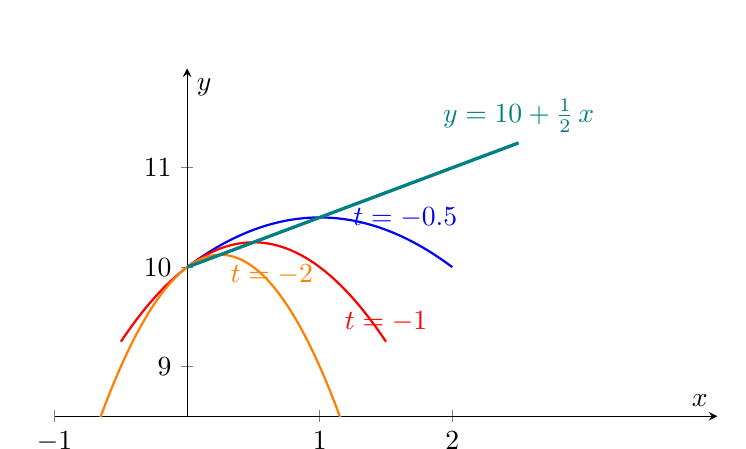
\begin{tikzpicture}
  \begin{axis}[
    axis lines=middle,
    xlabel={$x$}, ylabel={$y$},
    xmin=-1, xmax=4,
    ymin=8.5, ymax=12,
    xtick={-1,0,1,2}, ytick={9,10,11},
    domain=-1:2.5,
    samples=100,
    width=10cm,height=6cm,
  ]
    % Familia de parábolas limitadas alrededor de su punto de tangencia
    \addplot[blue, thick, domain=0:2]      {-0.5*x^2 + x + 10}  node[above,pos=0.8] {$t=-0.5$};
    \addplot[red, thick, domain=-0.5:1.5] {-1.0*x^2 + x + 10}  node[above,pos=1] {$t=-1$};
    \addplot[orange, thick, domain=-0.75:1.25] {-2.0*x^2 + x + 10} node[below right, pos =0.5] {$t=-2$};

    % Envolvente como función de x
    \addplot[teal, very thick, domain=0:2.5] {10 + 0.5*x} node[above,pos=1] {$y=10+\tfrac12\,x$};
  \end{axis}
\end{tikzpicture}
\end{center}


\subsection*{Ejemplo económico: maximización de beneficios sin restricciones}

Consideremos una empresa que produce una cantidad \(q\ge0\) de un bien y enfrenta un precio de mercado \(p>0\). Su beneficio \(\pi\) viene dado por
\[
\pi(q; p) \;=\; p\,q \;-\; C(q)
\]
donde \(C(q)\) es su función de costes, asumida de clase \(C^2\) y estrictamente convexa (\(C''(q)>0\))  

\subsubsection*{Problema de optimización}

Para cada precio \(p\) la empresa elige \(q\) para
\[
\max_{q\ge0}\;\pi(q;p)
\]
Las condiciones de primer y segundo orden son:
\[
\frac{\partial\pi}{\partial q}
= p - C'(q) = 0
\quad\Longrightarrow\quad
C'(q^*)=p
\]
\[
\frac{\partial^2\pi}{\partial q^2}
= -\,C''(q^*) < 0
\quad\Longrightarrow\quad
\text{\(\pi\) es cóncava en \(q\) y \(q^*(p)\) es el único máximo}
\]




%%%%%%%%%%%%%%%%%
\subsubsection*{Función de beneficio indirecto}

Definimos la función valor (beneficio máximo) como
\[
\Pi(p) \;=\;\pi\bigl(q^*(p);p\bigr)
= p\,q^*(p) - C\bigl(q^*(p)\bigr)
\]

\subsubsection*{Teorema de la envolvente}

Al derivar \(\Pi(p)\) con respecto a \(p\), aplicando el teorema de la envolvente se obtiene
\[
\frac{d\Pi}{dp}
= \frac{\partial\pi}{\partial p}\Bigl(q^*(p);p\Bigr)
= q^*(p)
\]
sin necesidad de calcular \(\tfrac{dq^*}{dp}\), pues \(\partial\pi/\partial q=0\) en el óptimo  

\subsubsection*{Función concreta}

Supongamos \(C(q)=\tfrac12\,c\,q^2\) con \(c>0\). Entonces
\[
C'(q)=c\,q\quad C''(q)=c>0
\]
y la condición de primer orden \(p=c\,q\) da
\[\color{teal}
q^*(p)=\frac{p}{c}\qquad \Pi(p)=p\cdot\frac{p}{c}-\tfrac12\,c\bigl(\tfrac{p}{c}\bigr)^2
=\frac{p^2}{2c}
\]
Verifiquemos la envolvente:
\[\color{teal}
\frac{d\Pi}{dp}
=\frac{d}{dp}\Bigl(\tfrac{p^2}{2c}\Bigr)
=\frac{p}{c}
=q^*(p)
\]

\subsubsection*{Interpretación}

\begin{itemize}
  \item La condición de envolvente \(\partial\pi/\partial q=0\) nos da la oferta óptima
    \(q^*(p)\)
  \item El teorema de la envolvente permite calcular la sensibilidad del beneficio máximo
    al precio \(p\) simplemente con \(\partial\pi/\partial p = q\), sin derivar la curva
    de oferta \(q^*(p)\). En este caso el resultado nos sugiere que ante un aumento del precio de venta, el beneficio máximo se incrementa.
\end{itemize}

\subsection*{Otro ejemplo económico: minimización de costes sujeto a restricción.}

Consideremos una empresa cuya tecnología de producción viene dada por la función Cobb–Douglas
\[
y = F(L,K) = L^\alpha K^{1-\alpha}
\qquad \alpha\in(0,1)
\]
donde \(L\) y \(K\) son trabajo y capital, y \(y>0\) es el nivel de output  

\subsubsection*{Problema de minimización de costes}

Dados los precios de los factores \(w\) (salario) y \(r\) (renta del capital) y el nivel \(y\), la empresa resuelve
\[
\min_{L,K}\;\; C = w\,L \;+\; r\,K
\quad\text{sujeto a}\quad
L^\alpha K^{1-\alpha} = y
\]

\subsubsection*{Demanda condicionada y coste mínimo}

Escribimos el Lagrangiano
\[
\mathcal L = wL + rK + \mu\bigl(y - L^\alpha K^{1-\alpha}\bigr)
\]
Las condiciones de primer orden son
\[
\frac{\partial\mathcal L}{\partial L}
= w - \mu\,\alpha\,L^{\alpha-1}K^{1-\alpha} = 0
\qquad
\frac{\partial\mathcal L}{\partial K}
= r - \mu\,(1-\alpha)\,L^\alpha K^{-\alpha} = 0
\]
junto con la restricción \(L^\alpha K^{1-\alpha}=y\). De las dos primeras:
\[
\frac{w}{\alpha}L^{1-\alpha}K^{\alpha-1}
\;=\;
\frac{r}{1-\alpha}L^{-\alpha}K^\alpha
\quad\Longrightarrow\quad
\frac{L^*}{K^*} = \frac{\alpha}{1-\alpha}\,\frac{r}{w}
\]
Sustituyendo en \(L^{\alpha}K^{1-\alpha}=y\) y resolviendo se obtienen las demandas condicionadas
\[\color{teal}
L^*(w,r,y)
= y\;\biggl(\frac{\alpha}{w}\biggr)^{\!\alpha}\!\biggl(\frac{1-\alpha}{r}\biggr)^{\!1-\alpha}\alpha
\quad
K^*(w,r,y)
= y\;\biggl(\frac{\alpha}{w}\biggr)^{\!\alpha}\!\biggl(\frac{1-\alpha}{r}\biggr)^{\!1-\alpha}(1-\alpha)
\]
El coste mínimo resultante es
\[\color{teal}
C(w,r,y)
= w\,L^*(w,r,y) + r\,K^*(w,r,y)
= y\;\Bigl(\tfrac{w}{\alpha}\Bigr)^{\!\alpha}
        \Bigl(\tfrac{r}{1-\alpha}\Bigr)^{\!1-\alpha}
\]

\subsubsection*{Lema de Shephard}

La función de coste \(C(w,r,y)\) es la envolvente de la familia de funciones \(wL + rK\) sujeta a \(F(L,K)=y\)  
Por el teorema de la envolvente, al derivar \(C\) con respecto a \(w\) (tratando \(y,r\) constantes) basta con tomar el efecto directo:
\[
\frac{\partial C}{\partial w}
= L^*(w,r,y)
\]
De hecho, si derivamos la expresión encontrada:
\[\color{teal}
\frac{\partial}{\partial w}
\Bigl[y\,(w/\alpha)^\alpha(r/(1-\alpha))^{1-\alpha}\Bigr]
= y\,\alpha\,(w/\alpha)^{\alpha-1}(r/(1-\alpha))^{1-\alpha}
= L^*(w,r,y)
\]
Análogamente,
\[\color{teal}
\frac{\partial C}{\partial r}
= K^*(w,r,y)
\]

\subsubsection*{Interpretación}

\begin{itemize}
  \item \(C(w,r,y)\) es la curva de coste de largo plazo: “envuelve” todas las rectas
    \(wL + rK\) tangentes a las iso-productivas \(L^\alpha K^{1-\alpha}=y\)  
  \item La envolvente simplifica el cálculo de las \emph{demandas condicionadas}: no necesitamos
    derivar \(L^*(w,r,y)\) ni \(K^*(w,r,y)\) respecto a \(w\) o \(r\) para obtener \(\partial C/\partial w\),
    \(\partial C/\partial r\)  
  \item \textbf{\color{teal}Este resultado se conoce como el Lema de Shephard}. El cual nos dice que una vez que tenemos la función de costo indirecta basta con derivar esta con respecto a los precios de los insumos para encontrar la demanda de insumos condicionada.
  \end{itemize}


\subsection*{Otro ejemplo: Monopolista multiproducto con dos bienes}

Sea un monopolista que ofrece dos bienes \(q_{1},q_{2}\ge0\) con demanda inversa lineal
\[
p_{1}(q_{1},q_{2}) = a - b\,q_{1} - c\,q_{2}
\quad
p_{2}(q_{1},q_{2}) = d - e\,q_{1} - f\,q_{2}
\]
y costos lineales
\[
C(q_{1},q_{2}) = g\,q_{1} + h\,q_{2}
\]
Entonces el beneficio es
\[
\pi(q_{1},q_{2})
= p_{1}\,q_{1} + p_{2}\,q_{2} - C(q_{1},q_{2})
= \bigl(a - bq_{1} - cq_{2}\bigr)q_{1}
+ \bigl(d - eq_{1} - fq_{2}\bigr)q_{2}
- \bigl(gq_{1} + hq_{2}\bigr)
\]

\subsubsection*{Condiciones de primer orden}

Para encontrar el máximo, derivamos la función de beneficio respecto a cada cantidad e igualamos a cero. \textbf{Es crucial incluir todos los términos cruzados.}

La derivada respecto a \(q_1\) es:
\[
\frac{\partial\pi}{\partial q_{1}}
= (a - 2b\,q_{1} - c\,q_{2}) + (-e\,q_2) - g = a - g - 2b\,q_{1} - (c+e)q_{2} = 0
\]
La derivada respecto a \(q_2\) es:
\[
\frac{\partial\pi}{\partial q_{2}}
= (-c\,q_1) + (d - e\,q_{1} - 2f\,q_{2}) - h = d - h - (c+e)q_{1} - 2f\,q_{2} = 0
\]
Esto nos da un sistema de dos ecuaciones lineales:
\[
\begin{cases}
2b\,q_{1} + (c+e)q_{2} = a - g \\
(c+e)q_{1} + 2f\,q_{2} = d - h
\end{cases}
\]

Resolviendo este sistema (por ejemplo, usando la regla de Cramer o sustitución) se obtienen las cantidades óptimas:
\[ \color{teal}
q_{1}^{*}
= \frac{2f\,(a - g) - (c+e)(d - h)}
{4bf - (c+e)^2}
\]
\[ \color{teal}
q_{2}^{*}
= \frac{2b\,(d - h) - (c+e)(a - g)}
{4bf - (c+e)^2}
\]

\subsubsection*{Condición de segundo orden (Hessiano)}

El Hessiano de \(\pi\) respecto a \((q_{1},q_{2})\) es:
\[
\nabla^{2}\pi
=
\begin{pmatrix}
\displaystyle \frac{\partial^{2}\pi}{\partial q_{1}^{2}}
& \displaystyle \frac{\partial^{2}\pi}{\partial q_{1}\partial q_{2}} \\[1em]
\displaystyle \frac{\partial^{2}\pi}{\partial q_{2}\partial q_{1}}
& \displaystyle \frac{\partial^{2}\pi}{\partial q_{2}^{2}}
\end{pmatrix}
=
\begin{pmatrix}
-2b & -(c+e) \\[0.5em]
-(c+e) & -2f
\end{pmatrix}
\]
Para que \((q_{1}^{*},q_{2}^{*})\) sea un máximo local, este Hessiano debe ser \textbf{definido negativo}:
\[
-2b < 0
\quad\Longrightarrow\quad
b>0
\]
y su determinante debe ser positivo:
\[
\det(\nabla^{2}\pi)
= (-2b)(-2f) - (-(c+e))(-(c+e))
= 4\,b\,f - (c+e)^{2}
>0
\]
Note que este denominador es el mismo que el utilizado para calcular $q_1^*$ y $q_2^*$.

\subsubsection*{Sensibilidad respecto de \(b\) y \(d\)}

Al aplicar el \textbf{teorema de la envolvente} al beneficio máximo \(\Pi(b,d)\), basta con derivar la función de beneficio \(\pi\) respecto a los parámetros \(b\) y \(d\), y luego evaluar en el punto óptimo \((q_{1}^{*},q_{2}^{*})\).

\[\color{teal}
\frac{\partial\pi}{\partial b}
= -\,q_{1}^{2}
\quad\Longrightarrow\quad
\frac{d\Pi}{db}
= -\,\bigl(q_{1}^{*}\bigr)^{2}
\]

\[\color{teal}
\frac{\partial\pi}{\partial d}
= q_{2}
\quad\Longrightarrow\quad
\frac{d\Pi}{dd}
= q_{2}^{*}
\]

\paragraph{Interpretación}

\begin{itemize}
  \item Un aumento de \(b\) (la demanda del bien 1 es más sensible a su propia cantidad) \textbf{reduce el beneficio máximo}, ya que \(\tfrac{d\Pi}{db}=-\,(q_{1}^{*})^{2}<0\).
  \item Un aumento de \(d\) (mayor disposición a pagar por el bien 2) \textbf{incrementa el beneficio máximo}, ya que se asume que la cantidad óptima \(\tfrac{d\Pi}{dd}=q_{2}^{*}\) será positiva.
\end{itemize}




\newpage
\section{Optimización con restricciones de igualdad}


\section*{Optimización con restricciones y Lagrangiano}

En muchos problemas de optimización no basta con minimizar (o maximizar) una función objetivo \(f\colon\mathbb{R}^n\to\mathbb{R}\) libremente: es preciso hacerlo sujeto a ciertas restricciones que deben cumplirse. En este apartado vamos a revisar el método de los \emph{multiplicadores de Lagrange} (o método del Lagrangiano) que es una herramienta fundamental para abordar problemas con restricciones de igualdad

\subsection*{Formulación del problema}

Consideremos el problema  
\[
\begin{aligned}
&\min_{x\in\mathbb{R}^n} f(x)\\
&\text{sujeto a}\quad g_i(x)=0,\quad i=1,\dots,k
\end{aligned}
\]
donde \(f\colon\mathbb{R}^n\to\mathbb{R}\), \(g_i\colon\mathbb{R}^n\to\mathbb{R}\) son funciones (\(C^1\)) y las curvas \(g_i(x)=0\) definen el conjunto factible.

\subsection*{El Lagrangiano}

Definimos la función Lagrangiana asociada al problema como  
\[\color{teal}
\mathcal{L}(x,\lambda)=f(x)+\sum_{i=1}^k\lambda_i\,g_i(x)
\]

El lagrangiano también puede formularse como:

\[\color{teal}
\mathcal{L}(x,\lambda)=f(x)-\sum_{i=1}^k\lambda_i\,g_i(x)
\]
Ya que el término $\lambda$ es una variable artificial que puede tener signo negativo o positivo. El resultado es indiferente de si aparece sumando o restando (de hecho véase que la restricción $g_i(x)=0$ puede multiplicarse ambos lados por $-1$ y sigue siendo  válida).

\subsection*{Condiciones de primer orden}

Un par \((x^*,\lambda^*)\) que resuelve el problema debe satisfacer las siguientes condiciones, que incluyen  
\begin{equation*}
\nabla_x \mathcal{L}(x^*,\lambda^*) = \nabla f(x^*) + \sum_{i=1}^k \lambda_i^*\,\nabla g_i(x^*)
\;=\;0
\label{eq:gradiente-zero}
\end{equation*}

\begin{equation*}
g_i(x^*)=0,\quad i=1,\dots,k
\label{eq:restricciones-cumplidas}
\end{equation*}

Estas condiciones son las mismas para maximizar o minimizar un problema de optimización libre. Por lo que el método del lagrangiano nos proporciona una simplificación del problema a cambio de agregar un multiplicador lagrangiano por cada restricción.

\subsection*{Interpretación geométrica}

Geométricamente, en el punto óptimo \(x^*\) el gradiente de la función objetivo debe poder expresarse como combinación lineal de los gradientes de las restricciones  
\[
\nabla f(x^*)\in\mathrm{span}\{\nabla g_1(x^*),\dots,\nabla g_k(x^*)\}
\]

\subsection*{Ejemplo: Minimización con restricción lineal}

Consideremos el problema  
\[
\begin{aligned}
&\min_{x,y\in\mathbb{R}} f(x,y)=x^2+y^2\\
&\text{sujeto a}\quad g(x,y)=x+y-1=0
\end{aligned}
\]

El Lagrangiano asociado es  
\[
\mathcal{L}(x,y,\lambda)=x^2+y^2-\lambda\,(x+y-1)
\]

Las condiciones de primer orden son  
\[
\frac{\partial \mathcal{L}}{\partial x}=2x-\lambda=0
\quad,\quad
\frac{\partial \mathcal{L}}{\partial y}=2y-\lambda=0
\quad,\quad
\frac{\partial \mathcal{L}}{\partial \lambda}=-(x+y-1)=0
\]
Es conveniente recordar que la condición  $\frac{\partial \mathcal{L}}{\partial \lambda}=0$ no es más que $g(x,y)=0$.\\
De las dos primeras ecuaciones se obtiene  
\[
x=\frac{\lambda}{2}
\quad,\quad
y=\frac{\lambda}{2}
\]
y sustituyendo en la restricción \(x+y=1\) resulta \(\lambda=1\) Por tanto  
\[
{\color{teal}x^*=y^*=\tfrac12}
\]
Este sería el candidato a óptimo ya que cumple las condiciones necesarias.

\subsection*{Otro ejemplo}

Consideremos el problema  
\[
\begin{aligned}
&\max_{x,y\in\mathbb{R}} f(x,y)=x\,y\\
&\text{sujeto a}\quad h(x,y)=x^2+y^2-1=0
\end{aligned}
\]

El Lagrangiano es  
\[
\mathcal{L}(x,y,\lambda)=x\,y-\lambda\bigl(x^2+y^2-1\bigr)
\]

Las condiciones de primer orden son  

\begin{equation}
\frac{\partial \mathcal{L}}{\partial x}=y-2\lambda\,x=0
\label{eq:L_x}
\end{equation}

\begin{equation}
\frac{\partial \mathcal{L}}{\partial y}=x-2\lambda\,y=0
\label{eq:L_y}
\end{equation}

\begin{equation}
\frac{\partial \mathcal{L}}{\partial \lambda}=-(x^2+y^2-1)=0
\label{eq:L_lambda}
\end{equation}

De \eqref{eq:L_x} y \eqref{eq:L_y} se deduce  
\[
y=2\lambda\,x
\quad,\quad
x=2\lambda\,y
\;\Longrightarrow\;
(2\lambda)^2=1
\;\Longrightarrow\;
\lambda=\pm\tfrac12
\]
Por la restricción \(x^2+y^2=1\) tenemos además  
\[
y=\pm x
\quad,\quad
x=\pm\tfrac{1}{\sqrt2}
\quad,\quad
y=\pm\tfrac{1}{\sqrt2}
\]
Así, los puntos críticos son  
\[\color{teal}
\Bigl(\tfrac1{\sqrt2},\,\tfrac1{\sqrt2}\Bigr),\;
\Bigl(-\tfrac1{\sqrt2},\,-\tfrac1{\sqrt2}\Bigr),\;
\Bigl(\tfrac1{\sqrt2},\,-\tfrac1{\sqrt2}\Bigr),\;
\Bigl(-\tfrac1{\sqrt2},\,\tfrac1{\sqrt2}\Bigr)
\]

Que serían candidatos a máximos y mínimos.
\subsection*{Ejemplo económico: Maximización de utilidad con restricción presupuestaria}

Consideremos un consumidor que elige cantidades \(x_1,x_2>0\) de dos bienes para maximizar su utilidad  
\[
u(x_1,x_2)=x_1^{\alpha}x_2^{1-\alpha}
\quad,\quad
\alpha\in(0,1)
\]
sujeto a su restricción presupuestaria  
\[
p_1\,x_1 + p_2\,x_2 = M
\]
donde \(p_1,p_2>0\) son los precios y \(M>0\) su ingreso

El Lagrangiano es  
\[
\mathcal{L}(x_1,x_2,\lambda)=x_1^{\alpha}x_2^{1-\alpha}+\lambda\bigl(M - p_1x_1 - p_2x_2\bigr)
\]

Las condiciones de primer orden son  

\begin{equation}
\frac{\partial\mathcal{L}}{\partial x_1}=\alpha\,x_1^{\alpha-1}x_2^{1-\alpha}-\lambda\,p_1=0
\label{FOC1}
\end{equation}

\begin{equation}
\frac{\partial\mathcal{L}}{\partial x_2}=(1-\alpha)\,x_1^{\alpha}x_2^{-\alpha}-\lambda\,p_2=0
\label{FOC2}
\end{equation}

\begin{equation}
\frac{\partial\mathcal{L}}{\partial \lambda}=M - p_1x_1 - p_2x_2=0
\label{FOC3}
\end{equation}

De \eqref{FOC1} y \eqref{FOC2} obtenemos  
\[
\frac{\alpha}{1-\alpha}\,\frac{x_2}{x_1}=\frac{p_1}{p_2}
\;\Longrightarrow\;
x_2=\frac{1-\alpha}{\alpha}\,\frac{p_1}{p_2}\,x_1
\]
Sustituyendo en \eqref{FOC3} y resolviendo, se llega a las demandas óptimas  
\[
{\color{teal}x_1^*=\frac{\alpha\,M}{p_1}}
\quad,\quad
{\color{teal}x_2^*=\frac{(1-\alpha)\,M}{p_2}}
\]




\section*{Condiciones de segundo orden}


Suponemos además que \(f\) y las \(g_i\) son de clase \(C^2\) en un entorno de \(x^*\).
\subsection*{Caso concreto: 2 variables independientes y una restricción}

Sea
\[
f:\R^2\to\R,
\quad
g:\R^2\to\R,
\quad
\mathcal L(x,y,\lambda)=f(x,y)+\lambda\,g(x,y).
\]
En un punto estacionario $(x^*,y^*,\lambda^*)$ se cumplen las condiciones de primer orden:
\[
\nabla f(x^*,y^*) \;=\;\lambda^*\,\nabla g(x^*,y^*),
\qquad
g(x^*,y^*)=0.
\]


Definimos las segundas derivadas de la función Lagrangiana
\(\mathcal L(x,y,\lambda)=f(x,y)+\lambda\,g(x,y)\) en el punto crítico \((x^*,y^*,\lambda^*)\) como

\[
\nabla^2_{(x,y,\lambda)}\mathcal L(x^*,y^*,\lambda^*)
=
\begin{pmatrix}
\mathcal L_{xx} & \mathcal L_{xy} & \mathcal L_{x\lambda} \\[6pt]
\mathcal L_{yx} & \mathcal L_{yy} & \mathcal L_{y\lambda} \\[6pt]
\mathcal L_{\lambda x} & \mathcal L_{\lambda y} & \mathcal L_{\lambda\lambda}
\end{pmatrix}_{(x^*,y^*,\lambda^*)}.
\]

Aquí,
\[
\begin{aligned}
\mathcal L_{xx}&=f_{xx}+\lambda^*\,g_{xx}, 
&\quad
\mathcal L_{xy}&=f_{xy}+\lambda^*\,g_{xy},\\
\mathcal L_{yx}&=f_{yx}+\lambda^*\,g_{yx}, 
&\quad
\mathcal L_{yy}&=f_{yy}+\lambda^*\,g_{yy},\\[4pt]
\mathcal L_{x\lambda}&=\,g_x,
&\quad
\mathcal L_{y\lambda}&=\,g_y,\\
\mathcal L_{\lambda x}&=\,g_x,
&\quad
\mathcal L_{\lambda y}&=\,g_y,\\[4pt]
\mathcal L_{\lambda\lambda}&=0
\end{aligned}
\]

Por tanto, al evaluar:
\[\color{teal}
\bar{H}=\nabla^2_{(x,y,\lambda)}\mathcal L(x^*,y^*,\lambda^*)
=
\begin{pmatrix}
f_{xx}+\lambda^*g_{xx} & f_{xy}+\lambda^*g_{xy} & \,g_x \\[6pt]
f_{yx}+\lambda^*g_{yx} & f_{yy}+\lambda^*g_{yy} & \,g_y \\[6pt]
\,g_x & \,g_y & 0
\end{pmatrix}_{(x^*,y^*,\lambda^*)}.
\]
La submatriz central de orden \(2\times2\) es precisamente las derivadas del lagrangiano con respecto a las variables $x,y$, y los elementos
\(g_x,g_y\) crean el “borde” que la convierte en el hessiano orlado.


\subsection*{Restricción lineal}
Cuando las restricciones son lineales el hessiano orlado se simplifica aún más: Supongamos 
\[
g(x,y)=a\,x + b\,y + c
\]
con \(a,b,c\) constantes. Entonces:

\begin{itemize}
  \item \(\displaystyle \nabla g(x,y) = (g_x, g_y) = (a, b)\): las primeras derivadas \(g_x=a\), \(g_y=b\) son constantes.
  \item Las segundas derivadas se anulan:
  \[
    g_{xx} = \frac{\partial}{\partial x}(g_x) = 0,
    \quad
    g_{xy} = \frac{\partial}{\partial y}(g_x) = 0,
    \quad
    g_{yy} = \frac{\partial}{\partial y}(g_y) = 0
  \]
\end{itemize}

Por tanto,
\[
\bar{H}=\nabla^2_{(x,y,\lambda)}\mathcal L(x^*,y^*,\lambda^*)
=
\begin{pmatrix}
f_{xx}+\lambda^*g_{xx} & f_{xy}+\lambda^*g_{xy} & \,g_x \\[6pt]
f_{yx}+\lambda^*g_{yx} & f_{yy}+\lambda^*g_{yy} &\,g_y \\[6pt]
\,g_x & \,g_y & 0
\end{pmatrix}_{(x^*,y^*,\lambda^*)}.
\]


los términos \(\,
\lambda\,g_{jk}\) desaparecen, y queda



\[
\bar{H}=\nabla^2_{(x,y,\lambda)}\mathcal L(x^*,y^*,\lambda^*)
=
\begin{pmatrix}
f_{xx} & f_{xy} &\,g_x \\[6pt]
f_{yx} & f_{yy} & \,g_y \\[6pt]
\,g_x & \,g_y & 0
\end{pmatrix}_{(x^*,y^*,\lambda^*)}.
\]





\subsection*{Condiciones suficientes para máximo o mínimo}

Sea en el punto crítico \((x^*,y^*,\lambda^*)\) el hessiano orlado
\[
\bar{H}(x^*,y^*,\lambda^*)
=
\begin{pmatrix}
0 & g_x & g_y \\[4pt]
g_x & f_{xx}+\lambda^*g_{xx} & f_{xy}+\lambda^*g_{xy} \\[4pt]
g_y & f_{yx}+\lambda^*g_{yx} & f_{yy}+\lambda^*g_{yy}
\end{pmatrix}_{(x^*,y^*,\lambda^*)}.
\]
Las condiciones suficientes para máximos y mínimos son:
\[\color{teal}
\det \bar{H}(x^*,y^*,\lambda^*) > 0
\quad\Longrightarrow\quad
\text{\((x^*,y^*)\) es un máximo local sujeto a }g=0
\]
\[\color{teal}
\det \bar{H}(x^*,y^*,\lambda^*) < 0
\quad\Longrightarrow\quad
\text{\((x^*,y^*)\) es un mínimo local sujeto a }g=0
\]

\subsection*{Condiciones suficientes: caso general}

Sea
\[
\begin{aligned}
&\min_{x\in\R^n} && f(x),\\
&\text{sujeto a} && g_i(x)=0,\quad i=1,\dots,k
\end{aligned}\]
o
\\
\[
\begin{aligned}
&\max_{x\in\R^n} && f(x),\\
&\text{sujeto a} && g_i(x)=0,\quad i=1,\dots,k
\end{aligned}
\]
y sea el Lagrangiano
\[
\mathcal L(x,\lambda)
\;=\;
f(x)\;+\;\sum_{i=1}^k\lambda_i\,g_i(x),
\qquad
\lambda=(\lambda_1,\dots,\lambda_k)
\]
Denotemos
\[
\nabla g(x)
\;=\;
\begin{pmatrix}
\nabla g_1(x) & \cdots & \nabla g_k(x)
\end{pmatrix}
\;\in\;\R^{n\times k}
\]
Suponiendo que $n>k$ (más variables independientes que restricciones). Entonces el \emph{hessiano orlado} se define como la matriz  
\((k+n)\times(k+n)\)
\[
\bar{H}(x,\lambda)
=
\begin{pmatrix}
0_{k\times k} & \nabla g(x)\\[6pt]
\nabla g(x)^{T}  & \nabla^2_{xx}\mathcal L(x,\lambda)
\end{pmatrix}
\]
Este hessiano orlado tiene asociado $n+k$ menores principales de orden inicial pero solo basta con analizar estos \(n-k\) últimos menores principales de orden inicial:

\begin{itemize}\color{teal}
  \item \textbf{Mínimo local}: si los últimos menores principales de orden inicial (líderes) tienen el signo de $(-1)^k$. Entonces \(x^*\) es \emph{mínimo} local sujeto a \(g_i=0\).
  \item \textbf{Máximo local}: Si los signos de los menores principales de orden inicial (líderes) se alternan terminando en el signo de $(-1)^n$ entonces \(x^*\) es \emph{máximo} local sujeto a \(g_i=0\).
\end{itemize}

Veamos ejemplos de esto:
\subsection*{En el caso de dos variables y una restricción, $k=1$, $n=2$ (analizado antes)}
Solo tenemos que analizar $2-1=1$ menor principal de orden inicial:
\begin{itemize}
  \item \textbf{Mínimo local}: si:
  \begin{equation*}
   |\bar{H}|
  \end{equation*}
  Tiene el signo de $(-1)^k=(-1)^1$ Es decir:
    \begin{equation*}
   |\bar{H}|<0
  \end{equation*}
  \item \textbf{Máximo local}:  si:
  \begin{equation*}
   |\bar{H}|
  \end{equation*}
  Tiene el signo de $(-1)^n=(-1)^2$ Es decir:
    \begin{equation*}
   |H|>0
  \end{equation*}
\end{itemize}

\subsection*{En el caso de tres variables y una restricción, $k=1$, $n=3$ }
El hessiano orlado asociado es el siguiente:
\[
\bar H(x^*,y^*,z^*,\lambda^*)
=
\begin{pmatrix}
0 & g_x & g_y & g_z \\[4pt]
g_x & f_{xx}+\lambda^*\,g_{xx} & f_{xy}+\lambda^*\,g_{xy} & f_{xz}+\lambda^*\,g_{xz} \\[4pt]
g_y & f_{yx}+\lambda^*\,g_{yx} & f_{yy}+\lambda^*\,g_{yy} & f_{yz}+\lambda^*\,g_{yz} \\[4pt]
g_z & f_{zx}+\lambda^*\,g_{zx} & f_{zy}+\lambda^*\,g_{zy} & f_{zz}+\lambda^*\,g_{zz}
\end{pmatrix}_{(x^*,y^*,z^*,\lambda^*)}
\]



Solo tenemos que analizar $3-1=2$ menores principales de orden inicial. Sean $ \Delta_1$ y $\Delta_2$ los últimos dos menores principales de orden inicial:
 \[
{
\Delta_1
=
\det
\begin{pmatrix}
0 & g_x & g_y \\
g_x & f_{xx}+\lambda^*\,g_{xx} & f_{xy}+\lambda^*\,g_{xy} \\
g_y & f_{yx}+\lambda^*\,g_{yx} & f_{yy}+\lambda^*\,g_{yy}
\end{pmatrix}
}
\]
 \[
{
\Delta_2
=
\det
\begin{pmatrix}
0 & g_x & g_y & g_z \\[4pt]
g_x & f_{xx}+\lambda^*\,g_{xx} & f_{xy}+\lambda^*\,g_{xy} & f_{xz}+\lambda^*\,g_{xz} \\[4pt]
g_y & f_{yx}+\lambda^*\,g_{yx} & f_{yy}+\lambda^*\,g_{yy} & f_{yz}+\lambda^*\,g_{yz} \\[4pt]
g_z & f_{zx}+\lambda^*\,g_{zx} & f_{zy}+\lambda^*\,g_{zy} & f_{zz}+\lambda^*\,g_{zz}
\end{pmatrix}_{(x^*,y^*,z^*,\lambda^*)}
}
\]

\begin{itemize}\color{teal}
  \item \textbf{Mínimo local}: si:
  \begin{equation*}
   \Delta_1, \Delta_2 
  \end{equation*}
  Tienen el mismo signo que $(-1)^k=(-1)^1$ es decir
 \begin{equation*}
   \Delta_1, \Delta_2 <0
  \end{equation*}
 
  \item \textbf{Máximo local}:  si:
  \begin{equation*}
   \Delta_1, \Delta_2 
  \end{equation*}
  Alternan el signo terminando con el signo de $(-1)^n=(-1)^3$ Es decir:
   \begin{equation*}
   \Delta_1 >0 
  \end{equation*}
     \begin{equation*}
    \Delta_2 <0
  \end{equation*}
\end{itemize}



\subsection*{En el caso de tres variables y dos restricciones, \(k=2\), \(n=3\)}

El hessiano orlado asociado en \((x^*,y^*,z^*,\lambda_1^*,\lambda_2^*)\) es  
\[
\bar H(x^*,y^*,z^*,\lambda_1^*,\lambda_2^*)
=
\begin{pmatrix}
0 & 0 & g_{1x} & g_{1y} & g_{1z} \\[4pt]
0 & 0 & g_{2x} & g_{2y} & g_{2z} \\[4pt]
g_{1x} & g_{2x} & f_{xx}+\lambda_1^*\,g_{1xx}+\lambda_2^*\,g_{2xx} & f_{xy}+\lambda_1^*\,g_{1xy}+\lambda_2^*\,g_{2xy} & f_{xz}+\lambda_1^*\,g_{1xz}+\lambda_2^*\,g_{2xz} \\[4pt]
g_{1y} & g_{2y} & f_{yx}+\lambda_1^*\,g_{1yx}+\lambda_2^*\,g_{2yx} & f_{yy}+\lambda_1^*\,g_{1yy}+\lambda_2^*\,g_{2yy} & f_{yz}+\lambda_1^*\,g_{1yz}+\lambda_2^*\,g_{2yz} \\[4pt]
g_{1z} & g_{2z} & f_{zx}+\lambda_1^*\,g_{1zx}+\lambda_2^*\,g_{2zx} & f_{zy}+\lambda_1^*\,g_{1zy}+\lambda_2^*\,g_{2zy} & f_{zz}+\lambda_1^*\,g_{1zz}+\lambda_2^*\,g_{2zz}
\end{pmatrix}
\]

Solo tenemos que analizar $(3-2)=1$ menor principal de orden inicial es decir $|\bar{H}|$.


\begin{itemize}\color{teal}
\item \textbf{Mínimo local}: si:
  \begin{equation*}
   |\bar{H}|
  \end{equation*}
  Tiene el signo de $(-1)^k=(-1)^2$ Es decir:
    \begin{equation*}
   |\bar{H}|>0
  \end{equation*}
  \item \textbf{Máximo local}:  si:
  \begin{equation*}
   |\bar{H}|
  \end{equation*}
  Tiene el signo de $(-1)^n=(-1)^3$ Es decir:
    \begin{equation*}
   |H|<0
  \end{equation*}
\end{itemize}


\section*{Condiciones para máximos y mínimos globales y únicos}
Al igual que en optimización no restringida es necesario especificar si la función es cóncava o convexa para la existencia de un máximo o mínimo global, con la optimización restringida ocurre lo mismo. Sea
\[
f: \mathbb{R}^n \;\longrightarrow\; \mathbb{R}
\]
la función objetivo y sea
\[
C \;=\; \bigl\{\,x \in \mathbb{R}^n : h_j(x)=0,\; j=1,\dots,p \bigr\}
\]
el conjunto factible. 
\subsection*{Condiciones para máximo global y único}


{\color{teal}Si \(f\) es estrictamente cuasicóncava y el conjunto factible \(C\) es convexo, entonces cualquier óptimo local del problema
  \[
    \max_{x\in C} \; f(x)
  \]
  es también óptimo global y único.}
 
\subsection*{Condiciones para mínimo global y único}

{\color{teal}Si \(f\) es estrictamente cuasiconvexa y el conjunto factible \(C\) es convexo, entonces cualquier óptimo local del problema
\[
  \min_{x\in C} \; f(x)
\]
es también óptimo global y único.}



\newpage
\section{Optimización con restricciones de desigualdad}



\section*{Problema con una sola variable independiente}

Consideremos el problema
\[
\max_{x\ge0}f(x),\qquad f\in C^1(\mathbb{R}).
\]
Un punto \(x^*\) es máximo local solo en una de estas dos situaciones:

\begin{itemize}
  \item \textbf{Interior:} \(x^*>0\) y \(f'(x^*)=0\). Aquí la restricción no interviene y se cumple la condición clásica de primer orden.
  \item \textbf{Frontera:} \(x^*=0\) y \(f'(0)\le0\).  
\end{itemize}

Obsérvese que \(f'(0)>0\) no puede corresponder a un máximo, pues implicaría pendiente creciente al inicio de la región factible.

Gráficamente los casos son los siguientes: $f'(x)=0$ por lo que la restricción no está activa.

\begin{center}
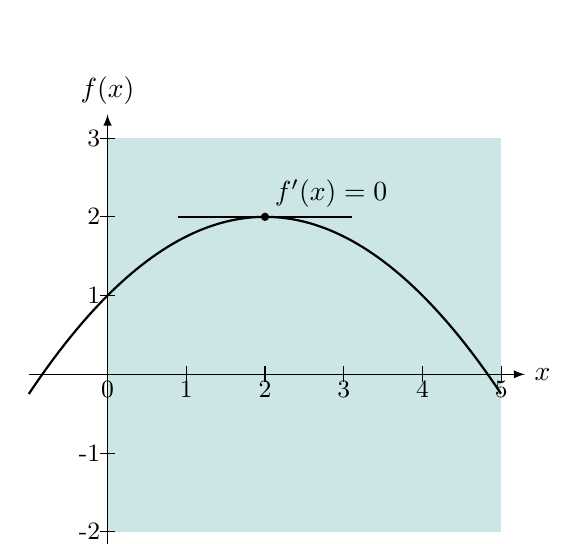
\begin{tikzpicture}[scale=1,>=latex]

  % Parámetros de la ventana gráfica
  \def\xmin{-1}
  \def\xmax{5}
  \def\ymin{-2}
  \def\ymax{3}

  % Región factible x1 >= 0 sombreada en teal
  \fill[teal,opacity=0.2] (0,\ymin) rectangle (\xmax,\ymax);

  % Ejes
  \draw[->] (\xmin,0) -- (\xmax+0.3,0) node[right] {$x$};
  \draw[->] (0,\ymin-0.3) -- (0,\ymax+0.3) node[above] {$f(x)$};
  \node[below left] at (0,0) {};

  % Marcas de escala en x y y
  \foreach \x in {0,1,2,3,4,5} {
    \draw (\x,0) ++(0,-0.1) -- ++(0,0.2) node[below,yshift=-2pt] {\small \x};
  }
  \foreach \y in {\ymin,-1,1,2,3} {
    \draw (0,\y) ++(-0.1,0) -- ++(0.2,0) node[left,xshift=-2pt] {\small \y};
  }

  % Función cóncava f(x1) = 2 - 0.25*(x1-2)^2
  \draw[thick,domain=\xmin:\xmax,samples=200,smooth]
    plot (\x,{2 - 0.25*(\x-2)^2});

  % Punto óptimo A en (2,2)
  \coordinate (A) at (2,2);
  \fill (A) circle (1.5pt) node[above right] {\(f'(x)=0\)};
  % Sublínea horizontal en A para ilustrar meseta
  \draw[-,thick] ($(A)+(-1.1,0)$) -- ($(A)+(1.1,0)$);

\end{tikzpicture}
\end{center}

Por otro lado $f'(x)<0$ implica que la restricción está activa: $x=0$.

\begin{center}
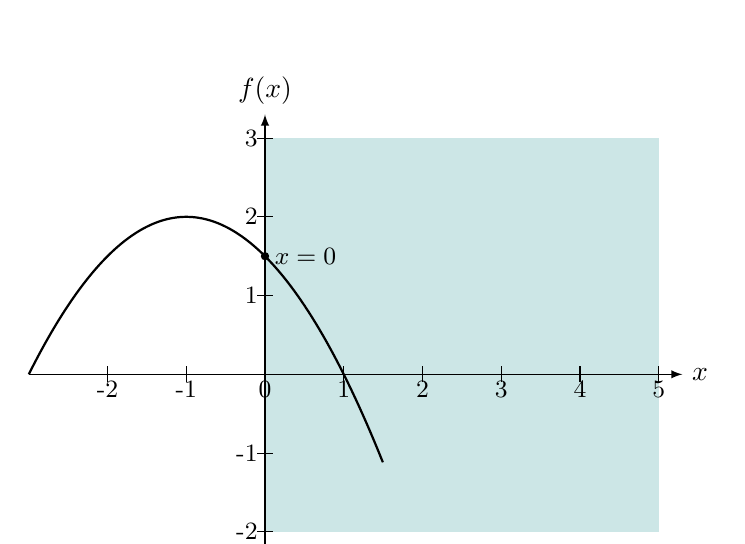
\begin{tikzpicture}[scale=1,>=latex]
  % Ventana gráfica
  \def\xmin{-3}
  \def\xmax{5}
  \def\ymin{-2}
  \def\ymax{3}

  % Región factible x >= 0 en teal semitransparente
  \fill[teal,opacity=0.2] (0,\ymin) rectangle (\xmax,\ymax);

  % Ejes
  \draw[->] (\xmin,0) -- (\xmax+0.3,0) node[right] {$x$};
  \draw[->] (0,\ymin-0.3) -- (0,\ymax+0.3) node[above] {$f(x)$};
  \node[below left] at (0,0) {};

  % Marcas de escala en x
  \foreach \x in {-2,-1,0,1,2,3,4,5}{
    \draw (\x,0) ++(0,-0.1) -- ++(0,0.2) node[below,yshift=-2pt]{\small \x};
  }
  % Marcas de escala en y
  \foreach \y in {\ymin,-1,1,2,3}{
    \draw (0,\y) ++(-0.1,0) -- ++(0.2,0) node[left,xshift=-2pt]{\small \y};
  }

  % Función cóncava con máximo en x=-1: f(x) = 2 - 0.5*(x+1)^2
  \draw[thick,domain=\xmin:1.5,samples=200,smooth]
    plot (\x,{2 - 0.5*(\x+1)^2});

  % Máximo no factible en (-1,2)
  \coordinate (M) at (0,1.5);
  \fill (M) circle (1.5pt) node[right] {\small \(x=0\)};

  % Línea de restricción x=0
  \draw[dashed] (0,\ymin) -- (0,\ymax) node[right,yshift=-4pt] {\small \(\)};
\end{tikzpicture}
\end{center}

Y por último también es posible que sucedan las dos cosas al mismo tiempo: $f'(x)=0$ y $x=0$.

\begin{center}
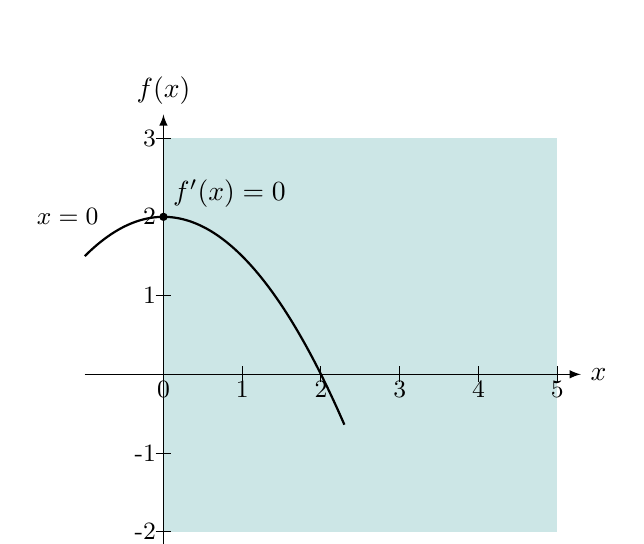
\begin{tikzpicture}[scale=1,>=latex]
  % Parámetros de la ventana gráfica
  \def\xmin{-1}
  \def\xmax{5}
  \def\ymin{-2}
  \def\ymax{3}

  % Región factible x >= 0 sombreada en teal
  \fill[teal,opacity=0.2] (0,\ymin) rectangle (\xmax,\ymax);

  % Ejes
  \draw[->] (\xmin,0) -- (\xmax+0.3,0) node[right] {$x$};
  \draw[->] (0,\ymin-0.3) -- (0,\ymax+0.3) node[above] {$f(x)$};
  \node[below left] at (0,0) {};

  % Marcas de escala en x y y
  \foreach \x in {0,1,2,3,4,5} {
    \draw (\x,0) ++(0,-0.1) -- ++(0,0.2) node[below,yshift=-2pt] {\small \x};
  }
  \foreach \y in {\ymin,-1,1,2,3} {
    \draw (0,\y) ++(-0.1,0) -- ++(0.2,0) node[left,xshift=-2pt] {\small \y};
  }

  % Función cóncava con máximo en x=0
  \draw[thick,domain=\xmin:2.3,samples=200,smooth]
    plot (\x,{2 - 0.5*(\x)^2});

  % Punto óptimo A en el borde (0,2)
  \coordinate (A) at (0,2);
  \fill (A) circle (1.5pt) node[above right] {\(f'(x)=0\)};
  % Línea punteada vertical indicando x=0 activo
  \draw[dashed] (A) -- (0,2) node[left,xshift=-20pt] {\small \(x=0\)};
\end{tikzpicture}
\end{center}


Estas condiciones anteriores pueden resumirse:
\[
f'(x)\le0,\quad x\ge0,\quad x\,f'(x)=0.
\]
De esas condiciones se deduce que necesariamente
\[
x=0\quad\text{o}\quad f'(x)=0,
\]
pues la última igualdad obliga a que al menos uno de los factores sea cero.

\begin{itemize}\color{teal}
  \item \(x\ge0\): 
  \item \(f'(x)\le0\): 
  \item \(x\,f'(x)=0\): \emph{holgura complementaria}.
\end{itemize}


\subsection*{Minimización}


Análogamente, para
\[
\min_{x\ge0}f(x),
\]
las condiciones necesarias son
\[\color{teal}
f'(x)\ge0,\quad x\ge0,\quad x\,f'(x)=0,
\]

\subsection*{Ejemplo}

Consideremos el problema
\[
\max_{x\ge0}f(x),
\quad
f(x) = -x^2 - x - 1,
\]


\textbf{Caso 1: la restricción está inactiva (óptimo interior).}\\
Si la restricción no actuase, existiría un máximo interior \(x^*>0\) y por lo tanto por la condición de holgura complementaria $x f'(x)=0$ tenemos que:
\[
f'(x^*) = 0.
\]
Pero
\[
f'(x) = -2x - 1,
\]
luego
\[
-2x^* - 1 = 0
\quad\Longrightarrow\quad
x^* = -\tfrac12,
\]
que contradice \(x^*>0\). Por tanto no puede haber óptimo interior en la región factible.

\medskip

\textbf{Caso 2: la restricción está activa (óptimo en la frontera).}\\
La única posibilidad restante es que \(x^*=0\). Para verificar que es un máximo local basta comprobar la condición de primer orden en la frontera:
\[
f'(0) = -2\cdot 0 - 1 = -1 \le 0.
\]

{\color{teal}Conclusión: En este ejemplo la restricción \(x\ge0\) está activa en el óptimo (\(x^*=0\)), y el valor óptimo es \(f(0)=-1<0\).}

Gráficamente:
\begin{center}
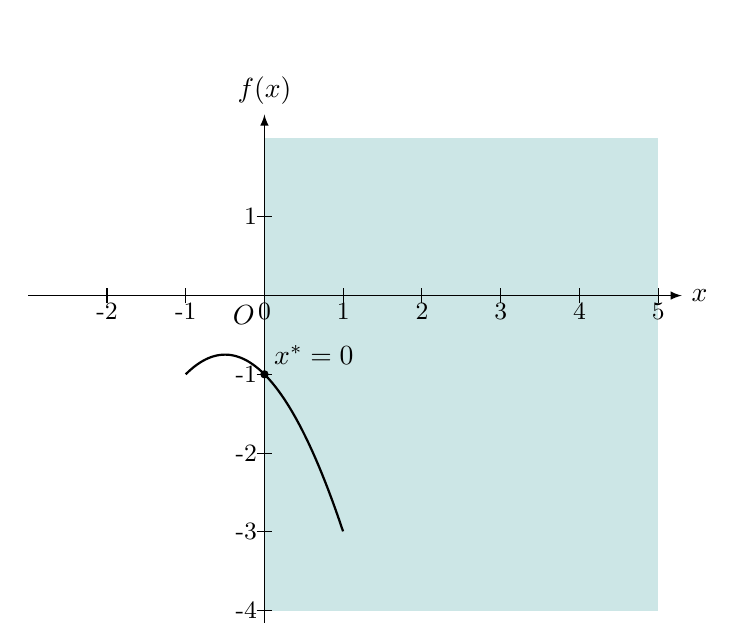
\begin{tikzpicture}[scale=1,>=latex]
  % Ventana gráfica
  \def\xmin{-3}
  \def\xmax{5}
  \def\ymin{-4}
  \def\ymax{2}

  % Región factible x >= 0 sombreada en teal
  \fill[teal,opacity=0.2] (0,\ymin) rectangle (\xmax,\ymax);

  % Ejes
  \draw[->] (\xmin,0) -- (\xmax+0.3,0) node[right] {$x$};
  \draw[->] (0,\ymin-0.3) -- (0,\ymax+0.3) node[above] {$f(x)$};
  \node[below left] at (0,0) {$O$};

  % Marcas de escala en x
  \foreach \x in {-2,-1,0,1,2,3,4,5}{
    \draw (\x,0) ++(0,-0.1) -- ++(0,0.2) node[below,yshift=-2pt]{\small \x};
  }
  % Marcas de escala en y
  \foreach \y in {\ymin,-3,-2,-1,1}{
    \draw (0,\y) ++(-0.1,0) -- ++(0.2,0) node[left,xshift=-2pt]{\small \y};
  }

  % Función cóncava f(x) = -x^2 - x - 1
  \draw[thick,domain=-1:1,samples=200,smooth]
    plot (\x,{ -(\x)^2 - (\x) - 1 });

  % Óptimo en la frontera (0,-1)
  \coordinate (A) at (0,-1);
  \fill (A) circle (1.5pt) node[above right] {\(x^*=0\)};
  
  % Línea de restricción x=0
  \draw[dashed] (0,\ymin) -- (0,\ymax) node[right,yshift=-4pt] {\small \(\)};
\end{tikzpicture}
\end{center}





\section*{Problema con n variables independientes y restricciones de no negatividad}



Consideremos
\[
\max_{x\in\mathbb R^n_+} \;f(x_1,\dots,x_n),\qquad f\in C^1(\mathbb R^n),
\]
es decir, sujeto a \(x_j\ge0\) para \(j=1,\dots,n\). 

Las condiciones de primer orden adaptadas a estas restricciones son, para cada \(j=1,\dots,n\):
\[
\frac{\partial f}{\partial x_j}
 \;\le\;0,\qquad
x_j\;\ge\;0,\qquad
x_j\,\frac{\partial f}{\partial x_j}
\;=\;0,
\]



\section*{Problema con tres variables y dos restricciones de desigualdad}

Planteamos primero el problema en forma de desigualdades:
\[
\max_{x_1,x_2,x_3}\;f(x_1,x_2,x_3)
\]
sujeto a
\[
\begin{cases}
g^1(x_1,x_2,x_3)\le r_1,\\
g^2(x_1,x_2,x_3)\le r_2,\\
x_1,\;x_2,\;x_3\ge0.
\end{cases}
\]
Al añadir las variables ficticias \(s_1,s_2\ge0\) podemos convertir cada desigualdad en una igualdad:
\[
\begin{cases}
g^1(x_1,x_2,x_3) + s_1 = r_1,\\
g^2(x_1,x_2,x_3) + s_2 = r_2,\\
x_1,\;x_2,\;x_3,\;s_1,\;s_2\ge0.
\end{cases}
\]


\subsection*{Lagrangiano y condiciones de primer orden}

A partir del problema con variables de holgura  
\[
\begin{aligned}
\max_{x_1,x_2,x_3,s_1,s_2}\;&f(x_1,x_2,x_3)\\
\text{sujeto a}\quad 
&g^1(x_1,x_2,x_3)+s_1 = r_1,\\
&g^2(x_1,x_2,x_3)+s_2 = r_2,\\
&x_j\ge0\;(j=1,2,3),\quad s_i\ge0\;(i=1,2),
\end{aligned}
\]
definimos el \emph{Lagrangiano}
\[
\mathcal{L}(x,s,\lambda)
\;=\;
f(x_1,x_2,x_3)
\;+\;\lambda_1\bigl[r_1 - g^1(x_1,x_2,x_3) - s_1\bigr]
\;+\;\lambda_2\bigl[r_2 - g^2(x_1,x_2,x_3) - s_2\bigr].
\]
Aquí \(\lambda_1,\lambda_2\in\mathbb R\) son los multiplicadores asociados a las igualdades.

\bigskip
\paragraph{Condiciones de primer orden}

\[
\begin{aligned}
\frac{\partial\mathcal L}{\partial x_1}
&= f_{1}(x)-\lambda_1\,g^1_{1}(x)-\lambda_2\,g^2_{1}(x)
\;\le\;0,\quad
x_1\;\ge\;0,\quad
x_1\,\frac{\partial\mathcal L}{\partial x_1}=0,\\[6pt]
\frac{\partial\mathcal L}{\partial x_2}
&= f_{2}(x)-\lambda_1\,g^1_{2}(x)-\lambda_2\,g^2_{2}(x)
\;\le\;0,\quad
x_2\;\ge\;0,\quad
x_2\,\frac{\partial\mathcal L}{\partial x_2}=0,\\[6pt]
\frac{\partial\mathcal L}{\partial x_3}
&= f_{3}(x)-\lambda_1\,g^1_{3}(x)-\lambda_2\,g^2_{3}(x)
\;\le\;0,\quad
x_3\;\ge\;0,\quad
x_3\,\frac{\partial\mathcal L}{\partial x_3}=0,\\[6pt]
\frac{\partial\mathcal L}{\partial s_1}
&= -\lambda_1
\;\le\;0,\quad
s_1\;\ge\;0,\quad
s_1\,\frac{\partial\mathcal L}{\partial s_1}=0,\\[6pt]
\frac{\partial\mathcal L}{\partial s_2}
&= -\lambda_2
\;\le\;0,\quad
s_2\;\ge\;0,\quad
s_2\,\frac{\partial\mathcal L}{\partial s_2}=0,\\[6pt]
\frac{\partial\mathcal L}{\partial \lambda_1}
&= r_1 - g^1(x_1,x_2,x_3) - s_1 = 0,\\
\frac{\partial\mathcal L}{\partial \lambda_2}
&= r_2 - g^2(x_1,x_2,x_3) - s_2 = 0.
\end{aligned}
\]




\paragraph{Eliminación de las variables ficticias de las condiciones de primer orden\\}
Tomemos la condición respecto a un multiplicador de lagrange:
\[
\frac{\partial\mathcal L}{\partial \lambda_i}
\;=\;
r_i - g^i(x_1,x_2,x_3) - s_i
\;=\;0,
\]
se despeja inmediatamente
\[
s_i \;=\; r_i - g^i(x_1,x_2,x_3),
\qquad i=1,2.
\]
Ahora sustituimos \(s_i\) en las tres condiciones
\[
\frac{\partial\mathcal L}{\partial s_i}\le0,\quad
s_i\ge0,\quad
s_i\,\frac{\partial\mathcal L}{\partial s_i}=0,
\]
recordando que \(\partial\mathcal L/\partial s_i=-\lambda_i\). Obtenemos:

\[
\begin{aligned}
-\lambda_i &\le0
&&\Longrightarrow\quad \lambda_i\ge0,\\
r_i - g^i(x_1,x_2,x_3) &\ge0
&&\\
\bigl(r_i - g^i(x_1,x_2,x_3)\bigr)\,\bigl(-\lambda_i\bigr)&=0
&&\Longrightarrow\quad \lambda_i\,(r_i - g^i(x_1,x_2,x_3))=0.
\end{aligned}
\]

En consecuencia, las condiciones de Kuhn-Tucker quedan:

\[\color{teal}
\begin{cases}
\displaystyle \frac{\partial\mathcal L}{\partial x_j}\;\le\;0,\\[4pt]
x_j\;\ge\;0,\\[4pt]
x_j\;\displaystyle\frac{\partial\mathcal L}{\partial x_j}\;=\;0
\end{cases}
\quad(j=1,2,3)
\]
\[\color{teal}
\begin{cases}
\displaystyle r_i - g^i(x_1,x_2,x_3)\;\ge\;0,\\[4pt]
\lambda_i\;\ge\;0,\\[4pt]
\lambda_i\;\bigl[r_i - g^i(x_1,x_2,x_3)\bigr]\;=\;0
\end{cases}
\quad(i=1,2)
\]



Véase que $r_i - g^i(x_1,x_2,x_3) $ coincide con la derivada del lagrangiano sin incluir las variables ficticias $s_i.$ 
Entonces podemos expresar las condiciones de la siguiente manera:

\[ \color{teal}
\begin{aligned}
\frac{\partial\mathcal L}{\partial x_j}&\le0,\quad x_j\ge0,\quad x_j\,\frac{\partial\mathcal L}{\partial x_j}=0,\\
\frac{\partial\mathcal L}{\partial \lambda_i}&\ge0,\quad \lambda_i\ge0,\quad \lambda_i\,\frac{\partial\mathcal L}{\partial \lambda_i}=0,
\end{aligned}
\]
\section*{Resumen de las condiciones}

Sea  
\[
L(x,\lambda)
= f(x_1,\dots,x_n)
+ \sum_{i=1}^{k}\lambda_i\bigl[r_i - g^i(x_1,\dots,x_n)\bigr]
\]
el Lagrangiano asociado a  
\[
\max_{x\in\mathbb R^n_+}f(x)
\quad\text{sujeto a}\quad
g^i(x)\le r_i\;(i=1,\dots,k)
\]
donde  
\[
\mathbb R^n_+ = \{x\in\mathbb R^n : x_j\ge0\ \forall j=1,\dots,n\}
\]

Las condiciones de Kuhn–Tucker para un máximo son  
\[
\begin{cases}
\displaystyle
\frac{\partial L}{\partial x_j}\le0,\quad
x_j\ge0,\quad
x_j\,\frac{\partial L}{\partial x_j}=0
& j=1,\dots,n\\[8pt]
\displaystyle
\frac{\partial L}{\partial \lambda_i}\ge0,\quad
\lambda_i\ge0,\quad
\lambda_i\,\frac{\partial L}{\partial \lambda_i}=0
& i=1,\dots,k
\end{cases}
\]

\subsection*{Condiciones Kuhn-Tucker generales para un mínimo}

Sea  
\[
L(x,\lambda)
= f(x_1,\dots,x_n)
+ \sum_{i=1}^{k}\lambda_i\bigl[r_i - g^i(x_1,\dots,x_n)\bigr]
\]
el Lagrangiano asociado a  
\[
\min_{x\in\mathbb R^n_+}f(x)
\quad\text{sujeto a}\quad
g^i(x)\ge r_i\;(i=1,\dots,k)
\]
donde  
\[
\mathbb R^n_+ = \{x\in\mathbb R^n : x_j\ge0\ \forall j=1,\dots,n\}
\]

Las condiciones de Kuhn–Tucker necesarias para un mínimo son  
\[
\begin{cases}
\displaystyle
\frac{\partial L}{\partial x_j}\ge0,\quad
x_j\ge0,\quad
x_j\,\frac{\partial L}{\partial x_j}=0
& j=1,\dots,n\\[8pt]
\displaystyle
\frac{\partial L}{\partial \lambda_i}\le0,\quad
\lambda_i\ge0,\quad
\lambda_i\,\frac{\partial L}{\partial \lambda_i}=0
& i=1,\dots,k
\end{cases}
\]



\subsection*{Ejemplo maximización}


Consideremos
\[
\max_{x,y}\;U(x,y)=xy
\quad\text{sujeto a}\quad
\begin{cases}
x+y\le100,\\
x\le40,\\
x\ge0,\;y\ge0.
\end{cases}
\]
Asignamos multiplicadores \(\lambda_1,\lambda_2\ge0\) a las dos primeras desigualdades y construimos el Lagrangiano
\[
\mathcal L(x,y,\lambda_1,\lambda_2)
=xy
+\lambda_1\bigl(100 - x - y\bigr)
+\lambda_2\bigl(40 - x\bigr).
\]
Las condiciones de Kuhn-Tucker se agrupan en:

\[
\begin{aligned}
&\frac{\partial\mathcal L}{\partial x}
=y-\lambda_1-\lambda_2\;\le0,\quad
x\;\ge0,\quad
x\bigl(y-\lambda_1-\lambda_2\bigr)=0,\\
&\frac{\partial\mathcal L}{\partial y}
=x-\lambda_1\;\le0,\quad
y\;\ge0,\quad
y\bigl(x-\lambda_1\bigr)=0,\\
&\frac{\partial\mathcal L}{\partial\lambda_1}
=100 - x - y\;\ge0,\quad
\lambda_1\;\ge0,\quad
\lambda_1\bigl(100 - x - y\bigr)=0,\\
&\frac{\partial\mathcal L}{\partial\lambda_2}
=40 - x\;\ge0,\quad
\lambda_2\;\ge0,\quad
\lambda_2\bigl(40 - x\bigr)=0.
\end{aligned}
\]

Analizando las regiones:\\
En el óptimo \(x^*,y^*>0\) ya que de lo contrario la utilidad sería 0, entonces las dos primeras desigualdades se vuelven igualdades (por las condiciones de holgura complementaria)
  \[
  y^*-\lambda_1-\lambda_2=0,\quad
  x^*-\lambda_1=0.
  \]



Analizando las regiones, consideremos las cuatro combinaciones posibles de \(\lambda_1\) y \(\lambda_2\):

\begin{enumerate}[label=\textbf{Caso \arabic*:}]
  \item \(\lambda_1=0,\;\lambda_2=0\).\\
    Entonces
    \[
      \frac{\partial\mathcal L}{\partial x}=y\le0,
      \quad
      \frac{\partial\mathcal L}{\partial y}=x\le0
      \quad\Longrightarrow\quad x=y=0,
    \]
    con \(x,y\ge0\). Esto da \(U=0\), no es máximo interior con \(U>0\).  
    \emph{\color{teal}(Descartado.)}

  \item \(\lambda_1>0,\;\lambda_2=0\).\\
    Por holgura complementaria en \(x,y>0\):
    \[
      y-\lambda_1=0,\quad x-\lambda_1=0
      \quad\Longrightarrow\quad x=y=\lambda_1,
    \]
    y por la restricción activa \(x+y=100\):
    \[
      2\lambda_1=100\;\Rightarrow\;x=y=50,
    \]
    pero viola \(x\le40\).  
    \emph{\color{teal}(Descartado.)}

  \item \(\lambda_1=0,\;\lambda_2>0\).\\
    Holgura complementaria obliga
    \[
      40-x=0\;\Rightarrow\;x=40,
    \]
    Y yendo a la segunda condición tenemos: $x-\lambda_1=0$. Pero como $\lambda_1=0$ y $x=40$, esta condición no se cumple.
    \emph{\color{teal}(Descartado.)}

  \item \(\lambda_1>0,\;\lambda_2>0\).\\
    Ambas restricciones activas:
    \[
      x+y=100,\quad x=40
      \quad\Longrightarrow\quad (x,y)=(40,60).
    \]
    De las derivadas:
    \[
      x-\lambda_1=0\;\Rightarrow\;\lambda_1=40,
      \quad
      y-\lambda_1-\lambda_2=0\;\Rightarrow\;\lambda_2=20>0,
    \]
    todo consistente.  
    \(\color{teal}{x^*=40,\;y^*=60,\;U=2400.}\)
\end{enumerate}


\subsection*{Ejemplo minimización}

Consideremos el problema

\[
\min_{x_1,x_2}\;C(x_1,x_2) \;=\;(x_1-4)^2\;+\;(x_2-4)^2
\]
sujeto a
\[
\begin{cases}
2x_1 + 3x_2 \;\ge\;6,\\
-3x_1 - 2x_2\;\ge\;-12,\\
x_1\ge0,\;x_2\ge0.
\end{cases}
\]
Reescribimos las dos primeras como
\[
g_1(x)\equiv 6 - 2x_1 - 3x_2 \;\le\;0,
\quad
g_2(x)\equiv 3x_1 + 2x_2 - 12\;\le\;0,
\]
y asignamos multiplicadores \(\lambda_1,\lambda_2\ge0\). El Lagrangiano es
\[
\mathcal L
= (x_1-4)^2 + (x_2-4)^2
+ \lambda_1\,(6 - 2x_1 - 3x_2)
+ \lambda_2\,(3x_1 +2x_2 - 12).
\]

\paragraph{Condiciones de Kuhn-Tucker}

\[
\begin{cases}
\displaystyle
\frac{\partial\mathcal L}{\partial x_1}
=2(x_1-4)\;-\;2\lambda_1\;+\;3\lambda_2
\;\ge\;0,
\;x_1\ge0,
\;x_1\bigl[2(x_1-4)-2\lambda_1+3\lambda_2\bigr]=0,\\[6pt]
\displaystyle
\frac{\partial\mathcal L}{\partial x_2}
=2(x_2-4)\;-\;3\lambda_1\;+\;2\lambda_2
\;\ge\;0,
\;x_2\ge0,
\;x_2\bigl[2(x_2-4)-3\lambda_1+2\lambda_2\bigr]=0,\\[6pt]
g_1(x)=6-2x_1-3x_2\le0,\;\lambda_1\ge0,\;\lambda_1\,(6-2x_1-3x_2)=0,\\[4pt]
g_2(x)=3x_1+2x_2-12\le0,\;\lambda_2\ge0,\;\lambda_2\,(3x_1+2x_2-12)=0.
\end{cases}
\]
\paragraph{Análisis de casos}  
Primero pensemos el caso de $(4,4)$ que dada la función de costos puede ser un potencial óptimo. Sin embargo, $(4,4)$ viola $g_2$. Por lo que vamos a analizar los otros casos posibles, suponiendo que $x_1>0$ y $x_2>0$
\[
x_1>0\;\Longrightarrow\;\frac{\partial\mathcal L}{\partial x_1}=0,\quad
x_2>0\;\Longrightarrow\;\frac{\partial\mathcal L}{\partial x_2}=0,
\]
y de que las dos restricciones pueden estar activas o inactivas. Hay cuatro combinaciones de \(\lambda_1,\lambda_2\ge0\):

\begin{enumerate}[label=\textbf{Caso \arabic*:}]
  \item \(\lambda_1=0,\;\lambda_2=0\).\\
    De la derivada con respecto a $x_1$\(:2(x_1-4)=0\Rightarrow x_1=4\) y  
    \(2(x_2-4)=0\Rightarrow x_2=4\).  
    Pero la segunda restricción \(3x_1+2x_2\le12\) se viola ($20>12$).  
    \emph{\color{teal}Descartado.}

  \item \(\lambda_1>0,\;\lambda_2=0\).\\
    De las condiciones obtenemos que:
    \[
      2(x_1-4)-2\lambda_1=0\quad\bigl(x_1=4+\lambda_1\bigr),\qquad
      2(x_2-4)-3\lambda_1=0\quad\bigl(x_2=4+\tfrac32\lambda_1\bigr).
    \]
    Además, \(\lambda_1>0\) implica \(2x_1+3x_2=6\), que no admite \(\lambda_1>0\).  
    \emph{\color{teal}Descartado.}

  \item \(\lambda_1=0,\;\lambda_2>0\).\\
    \[
     2(x_1-4)+3\lambda_2=0\;\Rightarrow\;x_1=4-\tfrac32\lambda_2,
    \]
    \[
     2(x_2-4)+2\lambda_2=0\;\Rightarrow\;x_2=4-\lambda_2,
    \]
    y \(\lambda_2>0\) obliga \(3x_1+2x_2=12\). Resolviendo:
    \[\color{teal}
      x_1=\frac{28}{13},\quad x_2=\frac{36}{13},\quad \lambda_2=\frac{16}{13}>0.
    \]
    Se verifica \(6-2x_1-3x_2<0\) (la primera restricción es inactiva).  
    \(\color{teal}{\text{\color{teal}Solución válida.}}\)

  \item \(\lambda_1>0,\;\lambda_2>0\).\\
    Ambas restricciones activas:
    \[
      2x_1+3x_2=6,\quad 3x_1+2x_2=12
      \;\Longrightarrow\;
      (x_1,x_2)=(\tfrac{24}{5},-\,\tfrac{6}{5}),
    \]
    que viola \(x_2\ge0\).  
    \emph{\color{teal}Descartado.}
\end{enumerate}

\noindent Por tanto, el único caso factible es \(\lambda_1=0,\;\lambda_2=\tfrac{16}{13}\), con  
\[\color{teal}
(x_1^*,x_2^*)=\Bigl(\tfrac{28}{13},\tfrac{36}{13}\Bigr).
\]


\section*{Condiciones suficientes}
Como en el caso de optimización con restricciones y optimización libre, las condiciones suficientes van a estar asociadas a la concavidad de las funciones analizadas. Vamos a ver dos tipos de condiciones, una sobre concavidad y convexidad y otra más débil sobre cuasiconcavidad y cuasiconvexidad.

\subsection*{Condiciones suficientes para máximo (y global)}
Supongamos que el problema a resolver es:
\[
\begin{aligned}
&\text{Maximizar} \quad  f(x) \\
&\text{sujeto a} \quad && g^{i}(x) \;\le\; r_{i}
\quad (i = 1,2,\dots,k),\\
& && x \;\ge\; 0.
\end{aligned}
\]
Con $x=(x_1,x_2,...)$
Asumiendo que se satisfacen las condiciones de Kuhn-Tucker.
Si se satisfacen las siguientes condiciones en un punto $x^*$
\begin{enumerate}\color{teal}
  \item La función objetivo \(f(x)\) es diferenciable y \emph{cóncava} en el cuadrante \(n\)-dimensional no negativo.
  \item Cada función de restricción \(g^{i}(x)\) es diferenciable y \emph{convexa} en el cuadrante \(n\)-dimensional no negativo.
\end{enumerate}
\textbf{\color{teal}Entonces \(x^{*}\) da un máximo global de \(f(x)\).}


Existe un teorema asociado a condiciones más débiles para poder determinar que estamos ante un máximo, estas están asociados a la cuasiconcavidad y cuasiconvexidad de las funciones:
\subsection*{Teorema de Arrow-Enthoven para máximo}
Supongamos que el problema a resolver es:

\[
\begin{aligned}
&\text{Maximizar} \quad f(x) \\
&\text{sujeto a} \quad && g^{i}(x) \;\le\; r_{i}
\quad (i = 1,2,\dots,k),\\
& && x \;\ge\; 0.
\end{aligned}
\]
Asumiendo que se satisfacen las condiciones de Kuhn-Tucker.
Si se satisfacen las siguientes condiciones en un punto $x^*$
\begin{enumerate}\color{teal}
  \item La función objetivo \(f(x)\) es diferenciable y \emph{cuasiconcava} en el cuadrante \(n\)-dimensional no negativo.
  \item Cada función de restricción \(g^{i}(x)\) es diferenciable y \emph{cuasiconvexa} en el cuadrante \(n\)-dimensional no negativo.
  \item Se satisface cualquiera de los siguientes:
    \begin{enumerate}
      \item \(f_{j}(x^{*}) < 0\) para al menos una variable \(x_{j}\).
      \item \(f_{j}(x^{*}) > 0\) para alguna variable \(x_{j}\) relevante, esto quiere decir una variable que en el conjunto factible (que cumpla con las restricciones), esa variable tome un valor positivo.
      \item Las \(n\) derivadas \(f_{j}(x^{*})\) no son todas cero, y la función \(f(x)\) es dos veces diferenciable en la vecindad de \(x^{*}\) (es decir, todas las derivadas parciales de segundo orden de \(f(x)\) existen para \(x^{*}\)).
      \item La función \(f(x)\) es cóncava.
    \end{enumerate}
\end{enumerate}

\textbf{\color{teal}Entonces \(x^{*}\) da un máximo global de \(f(x)\).
}



\subsection*{Condiciones suficientes para mínimo (y global)}
Supongamos que el problema a resolver es:
\[
\begin{aligned}
&\text{Minimizar} \quad  f(x) \\
&\text{sujeto a} \quad && g^{i}(x) \;\ge\; r_{i}
\quad (i = 1,2,\dots,k),\\
& && x \;\ge\; 0.
\end{aligned}
\]
Con $x=(x_1,x_2,...)$
Asumiendo que se satisfacen las condiciones de Kuhn-Tucker.
Si se satisfacen las siguientes condiciones en un punto $x^*$
\begin{enumerate}\color{teal}
  \item La función objetivo \(f(x)\) es diferenciable y \emph{convexa} en el cuadrante \(n\)-dimensional no negativo.
  \item Cada función de restricción \(g^{i}(x)\) es diferenciable y \emph{cóncava} en el cuadrante \(n\)-dimensional no negativo.
\end{enumerate}
\textbf{\color{teal}Entonces \(x^{*}\) da un mínimo global de \(f(x)\).}


\subsection*{Teorema de Arrow-Enthoven para mínimo}
Supongamos que el problema a resolver es:

\[
\begin{aligned}
&\text{Minimizar} \quad f(x) \\
&\text{sujeto a} \quad && g^{i}(x) \;\ge\; r_{i}
\quad (i = 1,2,\dots,k),\\
& && x \;\ge\; 0.
\end{aligned}
\]
Asumiendo que se satisfacen las condiciones de Kuhn-Tucker.
Si se satisfacen las siguientes condiciones en un punto $x^*$
\begin{enumerate}\color{teal}
  \item La función objetivo \(f(x)\) es diferenciable y \emph{cuasiconvexa} en el cuadrante \(n\)-dimensional no negativo.
  \item Cada función de restricción \(g^{i}(x)\) es diferenciable y \emph{cuasicóncava} en el cuadrante \(n\)-dimensional no negativo.
  \item Se satisface cualquiera de los siguientes:
    \begin{enumerate}
      \item \(f_{j}(x^{*}) > 0\) para al menos una variable \(x_{j}\).
      \item \(f_{j}(x^{*}) < 0\) para alguna variable \(x_{j}\) relevante, esto quiere decir una variable que en el conjunto factible (que cumpla con las restricciones), esa variable tome un valor positivo.
      \item Las \(n\) derivadas \(f_{j}(x^{*})\) no son todas cero, y la función \(f(x)\) es dos veces diferenciable en la vecindad de \(x^{*}\) (es decir, todas las derivadas parciales de segundo orden de \(f(x)\) existen para \(x^{*}\)).
      \item La función \(f(x)\) es convexa.
    \end{enumerate}
\end{enumerate}

\textbf{\color{teal}Entonces \(x^{*}\) da un mínimo global de \(f(x)\).
}


\end{document}
